\documentclass[12pt,a4paper,openright]{report}

\usepackage{xpatch}
\makeatletter


\xpatchcmd{\@part}{%
	\markboth{}{}% Find a hook in order to append content. 
}{%
	\markboth{}{}%
	\ifnum\c@secnumdepth>-2\relax
	\addcontentsline{lof}{part}{\thepart\hspace{1em}#1}%
	\else
	\addcontentsline{lof}{part}{#1}%
	\fi
}{\typeout{Success}}{\typeout{Patch failure}}


\xpatchcmd{\@part}{%
	\markboth{}{}% Find a hook in order to append content. 
}{%
	\markboth{}{}%
	\ifnum\c@secnumdepth>-2\relax
	\addcontentsline{lot}{part}{\thepart\hspace{1em}#1}%
	\else
	\addcontentsline{lot}{part}{#1}%
	\fi
}{\typeout{Success}}{\typeout{Patch failure}}
\makeatother


\usepackage{hyperref}

\usepackage{thesis}

\usepackage{url}
\usepackage{verbatim}
\usepackage{booktabs}  % See: http://texdoc.net/texmf-dist/doc/latex/booktabs/booktabs.pdf
\usepackage{todonotes} % Used for inserting comments inline or in the margins.

%%% Add any other packages you need to use here.
\usepackage{float}
\usepackage{makecell}
\usepackage{tabularx} 
\usepackage[T1]{fontenc}
\usepackage[tt=false, type1=true]{libertine}
\usepackage[varqu]{zi4} 
\usepackage[libertine]{newtxmath}
\usepackage{arabtex}
\usepackage{utf8}
%\usepackage[numbers, sort, comma, square]{natbib}
\usepackage[numbers, sort, comma, square]{natbib}
\usepackage{graphicx}
\usepackage{caption}
\usepackage{subcaption}
\usepackage{bm}
\usepackage{booktabs}
\usepackage{multirow}
% Tango imports the listings package and defines a style for syntax
% highlighting. We also need to tell listings which programming
% languages to load.
%
% This file defines a style for code listings, including syntax
% highlighting.
%

\usepackage{xcolor}
\definecolor{tenPercentGrey}{gray}{0.9}

% COLORS (Tango) Mostly by Philip Bunge
% http://pbunge.crimson.ch/
\definecolor{White}{gray}{0.9}
\definecolor{Black}{gray}{0.0}
\definecolor{LightButter}{rgb}{0.98,0.91,0.31}
\definecolor{LightOrange}{rgb}{0.98,0.68,0.24}
\definecolor{LightChocolate}{rgb}{0.91,0.72,0.43}
\definecolor{LightChameleon}{rgb}{0.54,0.88,0.20}
\definecolor{LightSkyBlue}{rgb}{0.45,0.62,0.81}
\definecolor{LightPlum}{rgb}{0.68,0.50,0.66}
\definecolor{LightScarletRed}{rgb}{0.93,0.16,0.16}
\definecolor{Butter}{rgb}{0.93,0.86,0.25}
\definecolor{Orange}{rgb}{0.96,0.47,0.00}
\definecolor{Chocolate}{rgb}{0.75,0.49,0.07}
\definecolor{Chameleon}{rgb}{0.45,0.82,0.09}
\definecolor{SkyBlue}{rgb}{0.20,0.39,0.64}
\definecolor{Plum}{rgb}{0.46,0.31,0.48}
\definecolor{ScarletRed}{rgb}{0.80,0.00,0.00}
\definecolor{DarkButter}{rgb}{0.77,0.62,0.00}
\definecolor{DarkOrange}{rgb}{0.80,0.36,0.00}
\definecolor{DarkChocolate}{rgb}{0.56,0.35,0.01}
\definecolor{DarkChameleon}{rgb}{0.30,0.60,0.02}
\definecolor{DarkSkyBlue}{rgb}{0.12,0.29,0.53}
\definecolor{DarkPlum}{rgb}{0.36,0.21,0.40}
\definecolor{DarkScarletRed}{rgb}{0.64,0.00,0.00}
\definecolor{Aluminium1}{rgb}{0.93,0.93,0.92}
\definecolor{Aluminium2}{rgb}{0.82,0.84,0.81}
\definecolor{Aluminium3}{rgb}{0.73,0.74,0.71}
\definecolor{Aluminium4}{rgb}{0.53,0.54,0.52}
\definecolor{Aluminium5}{rgb}{0.33,0.34,0.32}
\definecolor{Aluminium6}{rgb}{0.18,0.20,0.21}

%%% LISTINGS

\usepackage{listings}

\lstset{
  backgroundcolor=\color{tenPercentGrey}, %
  basicstyle=\color{Black}\ttfamily{}, %
  keywordstyle=[1]\color{DarkSkyBlue}, %
  keywordstyle=[2]\color{DarkScarletRed}, %
  keywordstyle=[3]\bfseries{}, %
  keywordstyle=[4]\color{DarkPlum}, %
  keywordstyle=[5]\color{SkyBlue}, %
  commentstyle=\color{Aluminium4}, %
  stringstyle=\color{Chocolate}, %
  identifierstyle=\color{Black}, %
  emphstyle=\color{Black}, %
  numbers=left, %
  stepnumber=1, % 
  frame=tb, %
  captionpos=b, %
  lineskip=\smallskipamount{}, %
  aboveskip=\bigskipamount{}, %
  belowskip=\medskipamount{}, %
  commentstyle=\itshape\small{}, %
  tabsize=2, %
  breaklines=false, %
  rulecolor=\color{Black!30}, %
  showspaces=false, %
  showstringspaces=false, %
  showtabs=false, %
} % chktex 6

\lstloadlanguages{Python,[LaTeX]TeX}

\makeatletter
\@addtoreset{chapter}{part}
\setcode{utf8}

%%% Set up the title page of the thesis.

\setuphyperref{Deep learning based Semantic Textual Similarity Metric for Applications in Translation Technology} {Tharindu Ranasinghe}

\begin{document}

%%% \thesistitle ends the preamble.
% Thesis title, author and name.
\thesistitle{Deep learning based Semantic Textual Similarity for Applications in Translation Technology} {Tharindu Ranasinghe} {2021}

%%% End of preamble.

% Thesis abstract.
\addcontentsline{toc}{chapter}{Abstract}

\chapter*{Abstract}




% Acknowledgements.
\addcontentsline{toc}{chapter}{Acknowledgements}

\chapter*{Acknowledgements}
This dissertation would not have been possible without the support of several wonderful people who helped me throughout my PhD studies. I have to keep this brief, and I hope I have not missed anyone of importance.

Firstly, I want to express my sincere gratitude to my Director of Studies Prof Ruslan Mitkov, from whom I have received invaluable advice and guidance throughout the course of my studies. He is the first person who encouraged me to employ deep learning in my study, and I came a long way following his advice. His insight and knowledge helped to shape the overall direction of the thesis. The continuous opportunities he provided me throughout the course helped me to grow as a researcher. I am very grateful for his continued encouragement and help in spite of his busy schedule.

I want to extend my sincere thanks to my first supervisor Prof Constantin Orăsan for his dedicated guidance, kindness, and support throughout my studies. His vision significantly influenced the direction of the research and the specifics of the technologies used in my experiments. His scientific and technical knowledge immensely benefited my work. Our regular meetings and conversations were always constructive and positive. Above everything, I want to thank him very much for being a friend more than a supervisor. The words can not describe my gratitude to him.

I am particularly grateful to Rocío Caro Quintana, Lucía Bellés Calvera and Encarnación Núñez Ignacio for providing evaluation support for Spanish sentences in translation memory experiments in this thesis. Their support helped me to complete the translation memory section successfully. I would also like to thank Dr María Navas Loro from Universidad Politécnica de Madrid for providing the tool she developed, Añotador, to extract dates from Spanish texts, which helped me to improve the results in translation memory experiments.


The Research Group in Computational Linguistics (RGCL) at the University of Wolverhampton is one of the best places in the world to study computational linguistics. I had the pleasure of meeting and forming friendships with many talented people from RGCL during this time. The collaborations I had with them helped to improve my technical skills. I am particularly grateful to all of my co-authors, Dr Marcos Zampieri, Alistair Plum, Dr Pablo Calleja, Dr Emad Mohamed, Zeses Pitenis, Hadeel Saadany and Salim Al Mandhari. I would also like to thank Dr Richard Evans, Dr Le An Ha, Dr Frédéric Blain, Dr Michael Oakes, Dr Burcu Can, Dr Omid Rohanian, Dr Maria Kunilovskaya, Dr Najah Albaqawi, Dr Sara Može and Dr Shiva Taslimipoor for having relaxing and informative discussions that helped me to improve my research at various points in my PhD. My time in England is my first time away from home. I want to thank Alistair Plum, Antonio Pascucci, Dr Marcos Zampieri and Dr Pablo Calleja for their friendship and support, which helped me settle down quickly in England.  

A special ‘thank you’ to Kate Wilson for proofreading the thesis and various research papers and providing English support which immensely helped me in writing my PhD. I would also like to thank Dr Amanda Bloore, Dr Emma Franklin, April Harper and Suman Hira for administrative support and proofreading papers at various points during my PhD. Their support made it possible for me to attend various conferences and complete my PhD smoothly.

None of these would be possible without emotional support. I want to thank my wife, Hansi Hettiarachchi, for being with me through thick and thin and for the various support she gave me throughout the course, including reading this thesis multiple times. Finally, I would like to thank my mother, father and sister for their unconditional love, blessings and support during the whole PhD.





% Automatically generated tables.
\singlespace{\tableofcontents}

\addcontentsline{toc}{chapter}{List of Tables}
\singlespace{\listoftables}

\newpage
\phantomsection \label{listoffig}
\addcontentsline{toc}{chapter}{List of Figures}
\singlespace{\listoffigures}

\addcontentsline{toc}{chapter}{List of Code Listings}
\singlespace{\lstlistoflistings}


\chapter{\label{cha:sts_introduction}Introduction}


\section{What is Semantic Textual Similarity?}

\section{Related Work}

\section{Datasets}
We experimented with several datasets throughout the experiments in the Semantic Textual Similarity Section. In order to maintain the versatility of our methods we experimented with several English datasets as well as several non English datasets and several datasets from different domains which we will introduce in this section.

\subsection{English Datasets}
\begin{enumerate}
  \item \textbf{SICK dataset} \footnote{The SICK dataset is available to download at \url{https://wiki.cimec.unitn.it/tiki-index.php?page=CLIC}} - The SICK data contains 9927 sentence pairs with a 5,000/4,927 training/test split which were employed in the SemEval 2014 Task1: Evaluation of Compositional Distributional Semantic Models on Full Sentences through Semantic Relatedness and Textual Entailment \cite{marelli-etal-2014-semeval}. The dataset has two types of annotations: Semantic Relatedness and Textual Entailment. We only use Semantic Relatedness annotations in our research. SICK was built starting from two existing datasets: the 8K ImageFlickr data set \footnote{The 8K ImageFlickr data set is available at \url{http://hockenmaier.cs.illinois.edu/8k-pictures.html}} \cite{rashtchian-etal-2010-collecting} and the SemEval-2012 STS MSR-Video Descriptions dataset \footnote{The SemEval-2012 STS MSR-Video Descriptions dataset is available at \url{https://www.cs.york.ac.uk/semeval-2012/task6/index.html}} \cite{agirre-etal-2012-semeval}. The 8K ImageFlickr dataset is a dataset of images, where each image is associated with five descriptions. To derive SICK sentence pairs the organisers randomly selected 750 images and sampled two descriptions from each of them. The SemEval2012 STS MSR-Video Descriptions data set is a collection of sentence pairs sampled from the short video snippets which compose the Microsoft Research Video Description Corpus \footnote{The Microsoft Research Video Description Corpus is available to download at \url{https://research.microsoft.com/en-us/downloads/38cf15fd-b8df-477e-a4e4-a4680caa75af/}}. A subset of 750 sentence pairs have been randomly chosen from this data set to be used in SICK. 
  
  In order to generate SICK data from the 1,500 sentence pairs taken from the source data sets, a 3-step process has been applied to each sentence composing the pair, namely \textit{(i) normalisation, (ii) expansion and (iii) pairing} \cite{marelli-etal-2014-semeval}. The \textit{normalisation} step has been carried out on the original sentences to exclude or simplify instances that contained lexical, syntactic or semantic phenomena such as named entities, dates, numbers, multiword expressions etc. In the \textit{expansion} step syntactic and lexical transformations with predictable effects have been applied to each normalized sentence, in
  order to obtain \textit{(i)} a sentence with a similar meaning, \textit{(ii)} a sentence with a logically contradictory or at least highly contrasting meaning, and \textit{(iii)} a sentence that contains most of the same lexical items, but has a different meaning. Finally, in the \textit{pairing} step each normalised sentence in the pair has been combined with all the sentences resulting from the expansion phase and with the other normalised sentence in the pair. Furthermore, a number of pairs composed of completely unrelated sentences have been added to the data set by randomly taking two sentences from two different pairs \cite{marelli-etal-2014-semeval}. 
  
  Each pair in the SICK dataset has been annotated to mark the degree to which the two sentence meanings are related (on a 5-point scale). The ratings 
  have been collected through a large crowdsourcing study, where each pair 
  has been evaluated by 10 different annotators. Once all the annotations were collected, the relatedness gold score has been computed for each pair as the average of the ten ratings assigned by the annotators \cite{marelli-etal-2014-semeval}. Table \ref{tab:sickdata} shows examples of sentence pairs with different degrees of semantic relatedness; gold relatedness scores are expressed on a 5-point rating scale.
  
  \begin{table}[ht!]
  	\centering 	
  	\begin{tabularx}{\textwidth}{l|c} 
  		\hline
  		\multicolumn{1}{c|}{\textbf{Sentence Pair}} & 
  		\multicolumn{1}{c}{\textbf{Relatedness}}  \\
  		\hline
  		\makecell[l]
  		{1. A little girl is looking at a woman in costume. \\ 
  		 2. A young girl is looking at a woman in costume.} & 4.7  \\
  		\hline
  			\makecell[l]
  		{1. Nobody is pouring ingredients into a pot. \\ 
  			2. Someone is pouring ingredients into a pot. } & 3.5  \\
  		\hline
  		\makecell[l]
  		{1. Someone is pouring ingredients into a pot. \\ 
  		 2. A man is removing vegetables from a pot. } & 2.8  \\
  		\hline
  		\makecell[l]
  		{1. A man is jumping into an empty pool. \\ 
  		 2. There is no biker jumping in the air. } & 1.6  \\
  		\hline               
  	\end{tabularx}
  	\caption[Example sentence pairs from the SICK dataset]{Example sentence pairs from the SICK dataset with their gold relatedness scores (on a 5-point rating scale).}
  	\label{tab:sickdata}
  \end{table}

 \item \textbf{STS 2017 English Dataset} \footnote{The STS 2017 English Dataset is available to download at \url{http://ixa2.si.ehu.es/stswiki/}} STS 2017 English Dataset was employed in SemEval-2017 Task 1: Semantic Textual Similarity Multilingual and Cross-lingual Focused Evaluation which is the most recent STS task in SemEval \cite{cer-etal-2017-semeval}.
  
 \item \textbf{Quora Question Pairs} \footnote{The Quora Question Pairs Dataset is available to download at \url{http://qim.fs.quoracdn.net/quora_duplicate_questions.tsv}}
 
  
\end{enumerate}

\section{Applications}

%%% The following are used by emacs, and similar:

%%% Local Variables: ***
%%% TeX-master: "../thesis.tex"  ***
%%% End: ***


\pagenumbering{arabic}\setcounter{page}{1}
\pagestyle{fancy}


% Your own thesis chapters go here.


\part{Semantic Textual Similarity}
\chapter{\label{cha:sts_introduction}Introduction}


\section{What is Semantic Textual Similarity?}

\section{Related Work}

\section{Datasets}
We experimented with several datasets throughout the experiments in the Semantic Textual Similarity Section. In order to maintain the versatility of our methods we experimented with several English datasets as well as several non English datasets and several datasets from different domains which we will introduce in this section.

\subsection{English Datasets}
\begin{enumerate}
  \item \textbf{SICK dataset} \footnote{The SICK dataset is available to download at \url{https://wiki.cimec.unitn.it/tiki-index.php?page=CLIC}} - The SICK data contains 9927 sentence pairs with a 5,000/4,927 training/test split which were employed in the SemEval 2014 Task1: Evaluation of Compositional Distributional Semantic Models on Full Sentences through Semantic Relatedness and Textual Entailment \cite{marelli-etal-2014-semeval}. The dataset has two types of annotations: Semantic Relatedness and Textual Entailment. We only use Semantic Relatedness annotations in our research. SICK was built starting from two existing datasets: the 8K ImageFlickr data set \footnote{The 8K ImageFlickr data set is available at \url{http://hockenmaier.cs.illinois.edu/8k-pictures.html}} \cite{rashtchian-etal-2010-collecting} and the SemEval-2012 STS MSR-Video Descriptions dataset \footnote{The SemEval-2012 STS MSR-Video Descriptions dataset is available at \url{https://www.cs.york.ac.uk/semeval-2012/task6/index.html}} \cite{agirre-etal-2012-semeval}. The 8K ImageFlickr dataset is a dataset of images, where each image is associated with five descriptions. To derive SICK sentence pairs the organisers randomly selected 750 images and sampled two descriptions from each of them. The SemEval2012 STS MSR-Video Descriptions data set is a collection of sentence pairs sampled from the short video snippets which compose the Microsoft Research Video Description Corpus \footnote{The Microsoft Research Video Description Corpus is available to download at \url{https://research.microsoft.com/en-us/downloads/38cf15fd-b8df-477e-a4e4-a4680caa75af/}}. A subset of 750 sentence pairs have been randomly chosen from this data set to be used in SICK. 
  
  In order to generate SICK data from the 1,500 sentence pairs taken from the source data sets, a 3-step process has been applied to each sentence composing the pair, namely \textit{(i) normalisation, (ii) expansion and (iii) pairing} \cite{marelli-etal-2014-semeval}. The \textit{normalisation} step has been carried out on the original sentences to exclude or simplify instances that contained lexical, syntactic or semantic phenomena such as named entities, dates, numbers, multiword expressions etc. In the \textit{expansion} step syntactic and lexical transformations with predictable effects have been applied to each normalized sentence, in
  order to obtain \textit{(i)} a sentence with a similar meaning, \textit{(ii)} a sentence with a logically contradictory or at least highly contrasting meaning, and \textit{(iii)} a sentence that contains most of the same lexical items, but has a different meaning. Finally, in the \textit{pairing} step each normalised sentence in the pair has been combined with all the sentences resulting from the expansion phase and with the other normalised sentence in the pair. Furthermore, a number of pairs composed of completely unrelated sentences have been added to the data set by randomly taking two sentences from two different pairs \cite{marelli-etal-2014-semeval}. 
  
  Each pair in the SICK dataset has been annotated to mark the degree to which the two sentence meanings are related (on a 5-point scale). The ratings 
  have been collected through a large crowdsourcing study, where each pair 
  has been evaluated by 10 different annotators. Once all the annotations were collected, the relatedness gold score has been computed for each pair as the average of the ten ratings assigned by the annotators \cite{marelli-etal-2014-semeval}. Table \ref{tab:sickdata} shows examples of sentence pairs with different degrees of semantic relatedness; gold relatedness scores are expressed on a 5-point rating scale.
  
  \begin{table}[ht!]
  	\centering 	
  	\begin{tabularx}{\textwidth}{l|c} 
  		\hline
  		\multicolumn{1}{c|}{\textbf{Sentence Pair}} & 
  		\multicolumn{1}{c}{\textbf{Relatedness}}  \\
  		\hline
  		\makecell[l]
  		{1. A little girl is looking at a woman in costume. \\ 
  		 2. A young girl is looking at a woman in costume.} & 4.7  \\
  		\hline
  			\makecell[l]
  		{1. Nobody is pouring ingredients into a pot. \\ 
  			2. Someone is pouring ingredients into a pot. } & 3.5  \\
  		\hline
  		\makecell[l]
  		{1. Someone is pouring ingredients into a pot. \\ 
  		 2. A man is removing vegetables from a pot. } & 2.8  \\
  		\hline
  		\makecell[l]
  		{1. A man is jumping into an empty pool. \\ 
  		 2. There is no biker jumping in the air. } & 1.6  \\
  		\hline               
  	\end{tabularx}
  	\caption[Example sentence pairs from the SICK dataset]{Example sentence pairs from the SICK dataset with their gold relatedness scores (on a 5-point rating scale).}
  	\label{tab:sickdata}
  \end{table}

 \item \textbf{STS 2017 English Dataset} \footnote{The STS 2017 English Dataset is available to download at \url{http://ixa2.si.ehu.es/stswiki/}} STS 2017 English Dataset was employed in SemEval-2017 Task 1: Semantic Textual Similarity Multilingual and Cross-lingual Focused Evaluation which is the most recent STS task in SemEval \cite{cer-etal-2017-semeval}.
  
 \item \textbf{Quora Question Pairs} \footnote{The Quora Question Pairs Dataset is available to download at \url{http://qim.fs.quoracdn.net/quora_duplicate_questions.tsv}}
 
  
\end{enumerate}

\section{Applications}

%%% The following are used by emacs, and similar:

%%% Local Variables: ***
%%% TeX-master: "../thesis.tex"  ***
%%% End: ***

\chapter{\label{cha:sts_state_of_the_art_methods}State of the Art Methods}

\section{Introduction}
\cite{ranasinghe-etal-2019-enhancing}
\section{Related Work}
\section{Improving State of the Art STS Methods}
\subsection{Portability to Other Languages}
\subsection{Portability to Other Domains}
\section{Conclusions}
\chapter{\label{cha:sts_sentence_encoders}Exploring STS with Sentence Encoders}

The main goal of a sentence encoder is to map a variable-length text to a fixed-length vector representation. In basic terms, a sentence encoder would take a sentence or text as the input and would output a vector. This vector encodes the meaning of the sentence and can be used for downstream tasks such as text classification, text similarity etc. In these down stream tasks, the sentence encoder is often considered as a black box where the users use the sentence encoder to get sentence embeddings without knowing what exactly happens in the encoder itself. 

Ideally, the approaches we experimented in Chapter \ref{cha:sts_state_of_the_art_methods} like Vector Averaging, Smooth Inverse Frequency \cite{DBLP:conf/iclr/AroraLM17} can also be considered as sentence encoders since in those approaches the input is a variable-length text and the output is a fixed-length vector. However, these approaches have major drawbacks in representing sentences. One such drawback is these approaches do not care about the word order. If you consider two sentences \textit{"Food is good but the service is bad"} and \textit{"Food is bad but the service is good"}, would have the same embeddings from these approaches even though the meaning of these two sentences is completely different. Another drawback is those approaches lose information in the vector aggregation process. If you consider two sentences \textit{"It is great"} and \textit{"It is not great"}, Vector Averaging and Smooth Inverse Frequency would give similar sentence embeddings as there is only one word difference in the two sentences. Even though this affect can be minimised using techniques like TF/IDF weighting that we explored in Chapter \ref{cha:sts_state_of_the_art_methods}, a different approach would be to train end-to-end models to get sentence embeddings. These models are commonly addressed as \textit{sentence encoders} in NLP community.

Over the years, various sentence encodes like Sent2vec \cite{pagliardini-etal-2018-unsupervised}, Infersent  \cite{cer2018universal}, Universal Sentence Encoder \cite{conneau-EtAl:2017:EMNLP2017} have been proposed. Even though most of these sentence encoders have sophisticated architectures, since many are using them only as a black box to get the sentence embeddings, they have been very popular in the NLP community. As the sentence encoders provide good quality sentence embeddings efficiently, the word embedding aggregation methods like Vector Averaging, Smooth Inverse Frequency have been often overlooked by the community in favour of sentence encoders. 

Once you have the sentence embedding from a sentence encoder, using them to calculate STS is an easy task. Since these sentence embeddings are already semantically powerful, a simple vector comparison technique like cosine similarity between the embeddings can be used to calculate the STS of the two sentences. Therefore, pre-trained sentence encoders can be used as an unsupervised STS method. However, even though the sentence encoders have been commonly used in STS tasks, there is no comprehensive study done on them. Since most of the researchers are using sentence encoders as a black box in many applications, they don't understand the limitations of using them. In this chapter we are addressing this gap by exploring sentence encoders in different STS datasets adopting them in different languages and domains. With a study like this we can understand the limitations of the sentence encoders and when not to use them. 

We address three research questions in this chapter:

\textbf{RQ1:} How well the sentence encoders perform in English STS datasets?

\textbf{RQ2:} Can the sentence encoders be easily adopted in different languages?

\textbf{RQ3:} How well the sentence encoders perform in different domains?

The main contributions of this chapter are as follows.

\begin{enumerate}
	\item In the Related Work Section (Section \ref{sec:sentence_related}), we discuss three sentence encoders that are popular in the NLP community. 
	
	\item  We evaluate these three sentence encoders on three English STS datasets, two non-English STS datasets and a bio-medical STS dataset which were introduced in Chapter \ref{cha:sts_introduction}.
	
	\item The code with the experiments conducted are publicly available to the community\footnote{The public GitHub repository is available on \url{https://github.com/tharindudr/simple-sentence-similarity}}.
	
\end{enumerate}

The rest of this chapter is organised as follows. Section \ref{sec:sentence_related} describes the three sentence encoders we experimented in this section. In Section \ref{sec:sentence_method} we present the experiments we conducted with the three sentence encoders in English STS datasets followed by the results comparing with the other unsupervised STS methods. Section \ref{sec:sentence_languages} and Section \ref{sec:sentence_domains} shows how sentence encoders can be applied to different languages and domains and their results. The chapter finishes with conclusions and ideas for future research directions in sentence encoders.


\section{Related Work}
\label{sec:sentence_related}
As we mentioned before, the sentence encoders are popular with the NLP community. The three sentence encoders explored in this chapter: Sent2vec \cite{pagliardini-etal-2018-unsupervised}, Infersent \cite{conneau-EtAl:2017:EMNLP2017} and Universal Sentence Encoder \cite{cer2018universal} are the most common sentence encoders. Other than them there is also Doc2vec \cite{pmlr-v32-le14} which is can be considered as a sentence encoder. However, due to the various upgrades in different python libraries, the official pre-trained Doc2vec models are not working any more. Therefore, we only used following sentence encoders in our experiments.

\paragraph{Sent2vec}
Sent2vec presents a simple but efficient unsupervised objective to train distributed representations of sentences \cite{pagliardini-etal-2018-unsupervised}. It can be thought as an extension of Word2vec (CBOW) to sentences. The key differences between CBOW and Sent2Vec are the removal of the input subsampling, considering the entire sentence as context, as well as the addition of word n-grams. With Sent2vec, sentence embedding is defined as the average of the word embeddings of its constituent words. The objective of Sent2vec is similar to CBOW; predict the missing word given the context \cite{pagliardini-etal-2018-unsupervised}. 

Sent2vec has officially released several pre-trained models to derive the sentence embeddings\footnote{The code and the pre-trained models are available on \url{https://github.com/epfml/sent2vec}}. Also due to its unsupervised approach and simple objective function, Sent2vec has been adopted in different languages and domains too.  


\paragraph{Infersent}
InferSent is an NLP technique for universal sentence representation developed by Facebook which uses supervised training to produce high quality sentence vectors \cite{conneau-EtAl:2017:EMNLP2017}. The authors explore 7 different architectures for sentence
encoding including LSTM \cite{10.1162/neco.1997.9.8.1735}, GRU \cite{Chung2014EmpiricalEO}, Bi directional LSTM \cite{650093} with mean/max pooling, Self-attentive network and Hierarchical Deep Convolutional Neural Network \cite{conneau-EtAl:2017:EMNLP2017}. All of these models were trained for the natural language inference (textual entailment) task using the architecture in Figure \ref{fig:infersent_general}. They evaluate the quality of the sentence representation by using them as features in 12 different transfer tasks like Binary and multi-class text classification, semantic textual similarity, paraphrase detection etc. The results indicate that the BiLSTM with the max-pooling operation performs best on these tasks  \cite{conneau-EtAl:2017:EMNLP2017}. The architecture of this BiLSTM with the max-pooling model is shown in Figure \ref{fig:infersent_architecture}.

Facebook released two models to derive the sentence embeddings. One model is trained with GloVe \cite{pennington-etal-2014-glove} which in turn has been trained on text preprocessed with the PTB tokeniser and the other model is trained with fastText \cite{mikolov-etal-2018-advances}  which has been trained on text preprocessed with the MOSES tokeniser. We used both models in our experiments\footnote{The code and the pre-trained models are available on \url{https://github.com/facebookresearch/InferSent}}.



\begin{figure}
	\captionsetup[subfigure]{justification=centering}
	\centering
	\begin{subfigure}[b]{.5\textwidth}
		\centering
		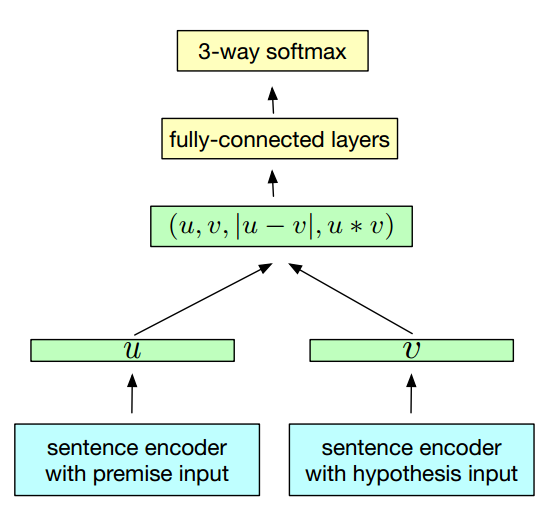
\includegraphics[width=\textwidth]{figures/semantic_textual_similarity/sentence_encoders/infersent_general.png}
		\caption{General NLI Training Scheme.}
		\label{fig:infersent_general}
	\end{subfigure}%
	\begin{subfigure}[b]{.5\textwidth}
		\centering
		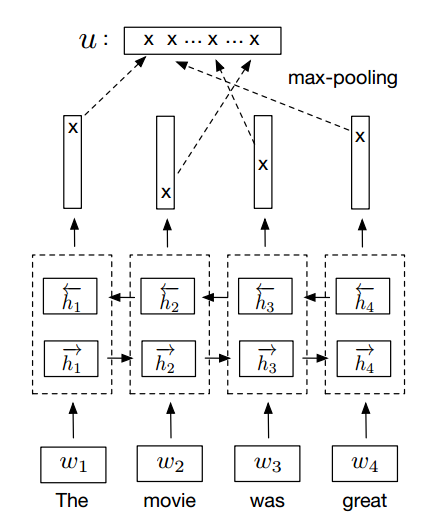
\includegraphics[width=\textwidth]{figures/semantic_textual_similarity/sentence_encoders/infersent.png}
		\caption{Bi directional LSTM  with max pooling}
		\label{fig:infersent_architecture}
	\end{subfigure}
	\caption[Infersent Architecture]{General NLI training scheme in Infersent with the best architecture; Bi directional LSTM  with max pooling \cite{conneau-EtAl:2017:EMNLP2017}. }
	\label{fig:infersent}
\end{figure}

\paragraph{Universal Sentence Encoder}

The Universal Sentence Encoder \cite{cer2018universal} released by Google is the last sentence encoder we employed in this chapter. This is again an unsupervised sentence encoder. It comes with two versions i.e. one trained with Transformer encoder and other trained with Deep Averaging Network
(DAN). Both architectures are outlined briefly below. The two have a trade-off of accuracy and computational resource requirement. While the one with Transformer encoder has higher accuracy, it is computationally more expensive. The one with DAN encoding is computationally less expensive but with slightly lower accuracy.

The original Transformer encoder model constitutes an encoder and decoder. Since our research is only focussed on encoding sentences to vectors, we only use its encoder part. The encoder is composed of a stack of N = 6 identical layers. Each layer has two sub-layers. The first is a multi-head self-attention mechanism, and the second is a simple, position-wise fully connected feed-forward network. \citet{cer2018universal} also employed a residual connection around each of the two sub-layers,
followed by layer normalisation. Since the model contains no recurrence and no convolution, for the model to make use of the order of the sequence, it must inject some information about the relative or absolute position of the tokens in the sequence, that is what the “positional encodings” does. The transformer-based encoder achieves the best overall transfer task performance. However, this comes at the cost of computing time and memory usage scaling dramatically with sentence length.

Deep Averaging Network (DAN) is much simpler where input embeddings for words and bi-grams are first averaged together and then passed through a feedforward deep neural network to produce sentence embeddings. The primary advantage of the DAN encoder is that computation time is linear in the length of the input sequence. With this sentence encoder too, we used both architectures in our experiments\footnote{Pre-trained sentence encoder for transformer model is available on \url{https://tfhub.dev/google/universal-sentence-encoder-large} and pre-trained sentence encoder for DAN model is available on \url{https://tfhub.dev/google/universal-sentence-encoder}.} Unlike the other sentence encoders, Google officially released two multilingual models for Universal Sentence Encoder.

\begin{figure}
	\captionsetup[subfigure]{justification=centering}
	\centering
	\begin{subfigure}[b]{.35\textwidth}
		\centering
		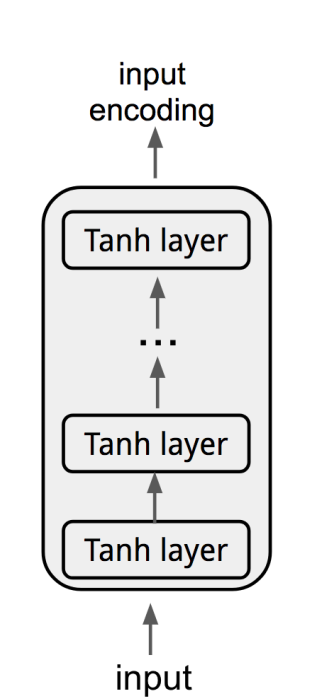
\includegraphics[width=\textwidth]{figures/semantic_textual_similarity/sentence_encoders/dan.png}
		\caption{DAN Architecture}
		\label{fig:dan}
	\end{subfigure}%
	\begin{subfigure}[b]{.35\textwidth}
		\centering
		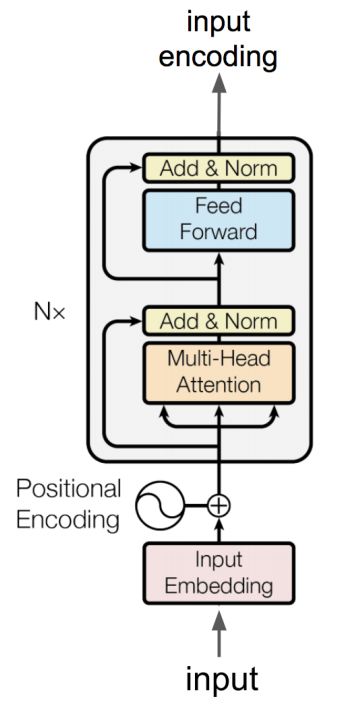
\includegraphics[width=\textwidth]{figures/semantic_textual_similarity/sentence_encoders/transformer.png}
		\caption{Transformer Architecture}
		\label{fig:transformer}
	\end{subfigure}
	\caption[Universal Sentence Encoder Architectures]{Two architectures in Universal Sentence Encoders.}
	\label{fig:use}
\end{figure}

\section{Exploring Sentence Encoders in English STS}
\label{sec:sentence_method}
Adopting sentence encoders for STS is an easy task.  If two embeddings from the two sentences are closer, the sentences are said to be semantically similar. As the approach, first the two sentences are passed to the sentence encoders to get the embeddings and the we calculate the cosine similarity between the resulting embeddings which represents the textual similarity of the two input sentences. To be clear, if the two vectors for two sentences X and Y are $a$ and $b$ correspondingly, we calculate the cosine similarity between $a$ and $b$ as of equation \ref{equ:cosine} and use that value to represent the similarity between the two sentences. 

\begin{equation}
	\label{equ:cosine}
	\begin{aligned}
		\cos ({\bf a},{\bf b})= {} & {{\bf a} {\bf b} \over \|{\bf a}\| \|{\bf b}\|} \\
		= {} & \frac{ \sum_{i=1}^{n}{{\bf a}_i{\bf b}_i} }{ \sqrt{\sum_{i=1}^{n}{({\bf a}_i)^2}} \sqrt{\sum_{i=1}^{n}{({\bf b}_i)^2}} }
	\end{aligned}
\end{equation}

First we experimented with English STS datasets we explained in Section \ref{sec:sts_intro_datsets}. For the experiments we used all the sentence encoders mentioned in Section \ref{sec:sentence_related}. For \textbf{Sent2vec}, we used the pre-trained Sent2vec model, \textit{sent2vec\_wiki\_bigrams} trained on English Wikipedia articles. Using that we could represent a sentence from a 700 dimensional vector. For \textbf{Infersent}, as we mentioned before, there are two pre-trained models available; \textit{infersent1} which was trained using GloVe \cite{pennington-etal-2014-glove} and \textit{infersent2} which was trained using fastText \cite{mikolov-etal-2018-advances}. Both models have been trained on the SNLI dataset which consists of 570k human generated English sentence pairs, manually labelled with one of the three categories: entailment, contradiction and neutral \cite{bowman-etal-2015-large}. Using that we could represent a sentence from a 512 dimensional vector. For \textbf{Universal Sentence Encoder}, we used universal-sentence-encoder (DAN architecture) and universal-sentence-encoder-large (Transformer architecture) which were trained on text resources like Wikipedia and news articles. With that too we could represent a sentence from a 512 dimensional vector.

We evaluated these three sentence encoders in three English STS datasets that we explained in Section \ref{sec:sts_intro_datsets}; SICK, STS2017 and QUORA.  Table \ref{tab:sick_sentence_encoder} shows the results for SICK dataset, Table \ref{tab:sts_sentence_encoder} shows the results for STS 2017 dataset and Table \ref{tab:quora_sentence_encoder} shows the results for Quora Questions Pairs dataset.


\begin{table*}[htb]
	%\footnotesize
	\centering
	\scalebox{0.95}{
		\begin{tabular}{|l|cc|}
			\hline
			\textbf{Model} & $\bm{\rho}$   & $\bm{\tau}$     
			\\ \hline
			\textit{ELMo $\bigoplus$ BERT}                     
			& 0.753  & 0.669       \\
			\hline
			\textit{Sent2vec}                     
			& 0.759  & 0.672      \\
			\hline
			\textit{Infersent1}                     
			& 0.763  & 0.679      \\\hline
			\textit{Infersent2}                     
			& 0.769  & 0.684      \\\hline
			\textit{USE (DAN)}                     
			& 0.772  & 0.695     \\\hline
			\textit{USE (Transformer)}                     
			& 0.780$^{\dagger}$  & 0.721$^{\dagger}$       \\
			
			\hline
		\end{tabular}
	}
	\caption[Results for SICK with sentence encoders]{Results for SICK dataset with sentence encoders. For each sentence encoder, Pearson Correlation ($\bm{\rho}$) and Spearman Correlation ($\bm{\tau}$) are reported between the predicted values and the gold labels of the test set. USE denotes Universal Sentence Encoder. Additionally, we report the results of the best model from Chapter \ref{cha:sts_state_of_the_art_methods}; \textit{ELMo $\bigoplus$ BERT}. Best result from all the methods is marked with ${\dagger}$. }  
	\label{tab:sick_sentence_encoder}
\end{table*}


\begin{table*}[htb]
	%\footnotesize
	\centering
	\scalebox{0.95}{
		\begin{tabular}{|l|cc|}
			\hline
			\textbf{Model} & $\bm{\rho}$   & $\bm{\tau}$     
			\\ \hline
			\textit{ELMo $\bigoplus$ BERT}                     
			& 0.654  & 0.616      \\
			\hline
			\textit{Sent2vec}                     
			& 0.673  & 0.645       \\
			\hline
			\textit{Infersent1}                     
			& 0.703  & 0.696       \\
			\hline
			\textit{Infersent2}                     
			& 0.711  & 0.701       \\
			\hline
			\textit{USE(DAN)}                     
			& 0.725  & 0.703       \\
			\hline
			\textit{USE(Transformer)}                     
			& 0.744$^{\dagger}$  & 0.721$^{\dagger}$       \\
			\hline
		\end{tabular}
	}
	\caption[Results for STS 2017 with sentence encoders]{Results for STS 2017 dataset with sentence encoders. For each sentence encoder, Pearson Correlation ($\bm{\rho}$) and Spearman Correlation ($\bm{\tau}$) are reported between the predicted values and the gold labels of the test set. USE denotes Universal Sentence Encoder. Additionally, we report the results of the best model from Chapter \ref{cha:sts_state_of_the_art_methods}; \textit{ELMo $\bigoplus$ BERT}. Best result from all the methods is marked with ${\dagger}$. }  
	\label{tab:sts_sentence_encoder}
\end{table*}


\begin{table*}[htb]
	%\footnotesize
	\centering
	\scalebox{0.95}{
		\begin{tabular}{|l|c|}
			\hline
			\textbf{Model} & RMSE     
			\\ \hline
			\textit{ELMo $\bigoplus$ BERT}                     
			& 0.566    \\
			\hline
			\textit{Sent2vec}                     
			& 0.632   \\
			\hline
			\textit{Infersent1}                     
			& 0.642    \\
			\hline
			\textit{Infersent2}                     
			& 0.653    \\
			\hline
			\textit{USE(DAN)}                     
			& 0.666    \\
			\hline
			\textit{USE(Transformer)}                     
			& 0.686$^{\dagger}$    \\
			
			\hline
		\end{tabular}
	}
	\caption[Results for QUORA with sentence encoders]{Results for QUORA dataset with sentence encoders. For each sentence encoder model, Root Mean Squared Error (RMSE) is reported. USE denotes Universal Sentence Encoder. Additionally, we report the results of the best model from Chapter \ref{cha:sts_state_of_the_art_methods}; \textit{ELMo $\bigoplus$ BERT}. Best result is marked with ${\dagger}$.}  
	\label{tab:quora_sentence_encoder}
\end{table*}

As can be seen in the results, Universal Sentence Encoder outperformed all other sentence encoders in all the English STS datasets. From the two architectures available in the Universal Sentence Encoder, Transformer architecture outperforms the DAN architecture as they have explained in their paper. Furthermore, it should be noted that in all three datasets, sentence encoders outperform the embedding aggregation based smooth inverse frequency method that performed best in Chapter \ref{cha:sts_state_of_the_art_methods}. This concludes that sentence encoders generally perform better than embedding aggregation techniques in STS. 

With these results, we can answer our \textbf{RQ1}, sentence encoders can be easily adopted and perform well in English STS tasks. However, most of these models are complex in nature which would result in more processing time/resources which can be chaotic in some situations. 


\section{Portability to Other Languages}
\label{sec:sentence_languages}
Our \textbf{RQ2} targets the multilinguality aspect of the sentence encoders; \textit{How well the sentence encoders perform in different languages?}. To answer this, we evaluated our method in Arabic STS and Spanish STS datasets that were introduced in Chapter \ref{cha:sts_introduction}. With these experiments, we identified a main weakness in sentence encoders; sentence encoders pre-trained on different languages are not easy to find. 

If you consider \textbf{Infersent}, it was pre-trained using the SNLI dataset which consists of 570k human generated English sentence pairs, manually labelled with one of three categories: entailment, contradiction and neutral \cite{bowman-etal-2015-large}. If someone is adopting \textbf{Infersent} for a different language other than English, they need to have a corpus similar to SNLI with a similar size. Annotating such a corpus for a different language would be challenging. Even though there are some attempts like XNLI \cite{conneau-etal-2018-xnli} to create such a corpus, the number of annotated instances are very limited. This makes it difficult to adopt \textbf{Infersent} in other languages which is a clear limitation of the Infersent architecture. 

However, the other two sentence encoders we experimented in this Chapter; Sent2vec and Universal Sentence Encoder are in a better position in multilingualism compared to Infersent as they don't require a large annotated corpus like SNLI. Both of those sentence encoders have been trained on unsupervised textual data which will be easy to find in most of the languages. However, still they need powerful computing resources to train the models which is a challenge when adopting these sentence encoders to different languages. 

For \textbf{Sent2Vec}, there was no Arabic pre-trained model available. However, there is a Spanish Sent2vec model\footnote{The pre-trained model is available on \url{https://github.com/BotCenter/spanish-sent2vec}} available which is pre-trained on Spanish Unannotated Corpora. Using that we could represent a Spanish sentence with a 700 dimensional vector. For \textbf{Universal Sentence Encoder}, there is a multilingual version which supports 16 languages\footnote{The model currently supports Arabic, Chinese-simplified, Chinese-traditional, English, French, German, Italian, Japanese, Korean, Dutch, Polish, Portuguese, Spanish, Thai, Turkish and Russian.} including Arabic and Spanish \cite{yang-etal-2020-multilingual}. This multilingual model is available in both architecture in Universal Sentence Encoder; DAN and Transformer\footnote{The multilingual Universal Sentence Encoder with DAN architecture is available on \url{https://tfhub.dev/google/universal-sentence-encoder-multilingual/3} and the multilingual Universal Sentence Encoder with Transformer architecture is available on \url{https://tfhub.dev/google/universal-sentence-encoder-multilingual-large/3}.}. Using that we could represent the Arabic and Spanish sentences with a 512 dimensional vector. As we mentioned before, for \textbf{Infersent}, we could not find any pre-trained models that supports either Arabic nor Spanish. Therefore, we did not use Infersent in our multilingual experiments. The Arabic and Spanish STS results with the mentioned sentence encoders are available in Table \ref{tab:arabic_spanish_sentence_encoder}.

\begin{table*}[htb]
	%\footnotesize
	\centering
	\scalebox{0.95}{
		\begin{tabular}{|c|c|c|c|}
			\hline
			\textbf{Language} &	\textbf{Sentence Encoder} &  $\bm{\rho}$ & $\bm{\tau}$     
			\\ \hline
			\multirow{ 3}{*}{\textit{Arabic}}	& \textit{ELMo $\bigoplus$ BERT}                    
			& 0.624 & 0.589 \\
			&	\textit{USE (DAN)}                     
			& 0.654 & 0.612 \\
			&	\textit{USE (Transformer)}                     
			& 0.668$^{\dagger}$ & 0.635$^{\dagger}$ \\
			\hline
				\multirow{ 4}{*}{\textit{Spanish}}	& \textit{ELMo $\bigoplus$ BERT}                    
			&  0.712 & 0.663\\
			&	\textit{USE (DAN)}                     
			& 0.723 & 0.6.682 \\
			& \textit{Sent2vec} & 0.725 & 0.688 \\
			&	\textit{USE (Transformer)}                     
			& 0.741$^{\dagger}$ & 0.702$^{\dagger}$ \\
			\hline
		\end{tabular}
	}
	\caption[Results for Arabic and Spanish STS with Sentence Encoders]{Results for Arabic and Spanish STS with different sentence encoders. For each sentence encoder, Pearson Correlation ($\bm{\rho}$) and Spearman Correlation ($\bm{\tau}$) are reported between the predicted values and the gold labels of the test set. USE denotes Universal Sentence Encoder. Additionally, we report the results of the best model from Chapter \ref{cha:sts_state_of_the_art_methods}; \textit{ELMo $\bigoplus$ BERT}. Best result for each language is marked with ${\dagger}$.}  
	\label{tab:arabic_spanish_sentence_encoder}
\end{table*}

As can be seen in results, similar to the English datasets, from the sentence encoders we considered,  Universal Sentence Encoder with the Transformer architecture gave the best results for both Arabic and Spanish datasets. From the two architectures available in the Universal Sentence Encoder, Transformer architecture outperforms the DAN architecture in both languages. Furthermore, it should be noted that in both languages, sentence encoders outperform the word embedding based smooth inverse frequency method that performed best in Chapter \ref{cha:sts_state_of_the_art_methods}.  

With these experiments, we can answer our \textbf{RQ2: How well the sentence encoders can be adopted in different languages?}. Adopting sentence encoders in different languages is challenging since there are no available pre-trained sentence encoder models for many languages. However, in the cases where they are available, it is very easy to use them in STS tasks and they provide good results compared to other unsupervised STS methods. 


\section{Portability to Other Domains}
\label{sec:sentence_domains}

In order to answer our \textit{RQ3}; how well the sentence encoders can be applied in different domains, we evaluated sentence encoders that we explained in this Chapter on the Bio-medical STS dataset explained in \ref{cha:sts_introduction}. As we mentioned before, Bio-medical STS dataset does not have a training set. Therefore, only the unsupervised approaches can be applied on this dataset which provides an ideal opportunity for the sentence encoders we experimented in this chapter. 

However, we faced the same issue we faced in Arabic and Spanish STS experiments in Bio-medical STS experiments too. There are not many options when it comes to sentence encoders that were trained on Bio-medical domain \cite{TAWFIK2020103396}. For \textbf{Sent2vec}, we could find a pre-trained model in Bio-medical domain which was trained using PubMed data \cite{8904728}\footnote{The code and the pre-trained model is available on \url{https://github.com/ncbi-nlp/BioSentVec}}. However, for other two sentence encoders, we could not find any available pre-trained sentence encoder models on Bio-medical domain. Therefore, for Universal Sentence Encoder and Infersent, we had to use pre-trained sentence encoder models trained on English texts for this experiments. The results are shown in Table \ref{tab:biosses_sentence_encoders}.

\begin{table*}[htb]
	%\footnotesize
	\centering
	\scalebox{0.95}{
		\begin{tabular}{|l|c|}
			\hline
			\textbf{Model} & $\bm{\rho}$   \\  
			\hline
			\textit{Infersent2} & 0.294 \\
			\textit{Infersent1} & 0.301 \\
			\textit{USE(DAN)} & o.321 \\
			\textit{USE(Transformer)} & 0.345 \\
			\textit{ELMo $\bigoplus$ BERT}  &  0.708 \\
			\textit{BioSentVec} \cite{8904728} & 0.810$^{\dagger}$  \\
			\hline
		\end{tabular}
	}
	\caption[Results comparison for BIOSSES with different sentence encoders]{Results for BIOSSES dataset with different sentence encoders compared with top results reported for BIOSSES. Additionally, we report the results of the best model from Chapter \ref{cha:sts_state_of_the_art_methods}; \textit{ELMo $\bigoplus$ BERT}. For each variant, Pearson Correlation ($\bm{\rho}$) is reported between the predicted values and the gold labels of the test set. Best result is marked with ${\dagger}$.}  
	\label{tab:biosses_sentence_encoders}
\end{table*} 

As can be observed in the results, sentence encoder trained on the Bio-medical domain; BioSentVec \cite{8904728} outperformed other approaches. In fact, when compared to the best results in the BIOSSES dataset BioSentVec outperforms all of them which means that BioSentVec provides the best result for BIOSSES. it should be noted that out of domain sentence encoders like Universal Sentence Encoder and Infersent, that were not trained on the Bio-medical domain performed very poorly in these experiments. The simple \textit{ELMo $\bigoplus$ BERT} embedding aggregation based approach we experimented in Chapter \ref{cha:sts_state_of_the_art_methods} outperforms Universal Sentence Encoder and Infersent by a large margin. This can be due to the fact that, there is a large number of out-of-vocabulary words for these general sentence coders in the Bio-medical domain unlike the \textit{ELMo $\bigoplus$ BERT} where we used the ELMo and BERT models trained on Bio-medical domain. We can conclude that sentence encoders can be successfully adopted for STS in different domains, however they won't succeed unless they are pre-trained on that particular domain. 

With these finding we answer our \textbf{RQ3: Is it possible to adopt sentence encoders in different domains?}. We showed that it is possible to adopt sentence encoders in a different domain. However, it is difficult since pre-trained sentence encoder models are not common in most domains and the sentence encoders pre-trained on a general domain perform poorly on a specific domain like Bio-medical. 

\section{Conclusions}
\label{sec:sentence_conclusions}
In this chapter we experimented another unsupervised STS method; sentence encoders. We explored three popular sentence encoders; Sent2vec, Infersent and Universal Sentence Encoder in three English STS datasets. The results show that sentence encoders outperforms other unsupervised STS methods. From the sentence encoders, Universal Sentence Encoder with the Transformer architecture performs best in all three datasets. Furthermore, we evaluated sentence encoders in different languages and domains. We experienced the biggest hurdle in adopting sentence encoders in different languages and domains; the pre-trained sentence encoders that support different languages and domains are not common compared to the word embedding/ contextual word embedding models available on those languages and domains. This is because the sentence encoders take a lot of time to train and some of the sentence encoders like Infersent require specific training data, which is hard to compile in most of the languages and domains. Also, since the applications of sentence encoders are limited compared to word embeddings/ contextual word embeddings people have not spend time on creating language specific and domain specific sentence encoders. However, when available they perform very well in the relevant tasks. Also we tried to use sentence encoders that were trained on a general domain in a different but specific domain like Bio-medical. This provided very poor results. Therefore, we can conclude that using sentence encoders on a different domain to their pre-trained domain won't provide good results.


Being an unsupervised STS method, the sentence encoders have the obvious advantage of not needing a training set for STS. However, they still need a pre-trained sentence encoding model, which is not available in most of the languages and domains. This is a major drawback in sentence encoders compared to the embedding aggregation methods since the word embedding/ contextual embedding models are commonly available in many languages and domains. This is worsened by the fact that sentence encoders perform very poorly on the domains that they did not see in the training process. This suggests that we should only use sentence encoders when available in a certain domain/ language, otherwise using embedding aggregation methods like Smooth Inverse Frequency would provide better results. 


As future work, the experiments can be extended in to recently released sentence encoders like LASER \cite{10.1162/tacl_a_00288}. LASER supports 93 languages including low resource languages like Kabyle, Malagasy, Sinhala etc. This should solve some of the multilingual issues we experienced with sentence encoders in this chapter. Very recently sentence encoders have been explored with Siamese neural architectures and  Transformers. We discuss them in Chapters \ref{cha:sts_siamese_neural_networks} and \ref{cha:sts_transformers}. 

\chapter{\label{cha:sts_siamese_neural_networks}Siamese Neural Networks for STS}

A \textit{Siamese Neural Network} refers to a class of neural network architecture that contains two or more identical subnetworks. This is usually employed in applications that require comparisons between two or more inputs (signature verification, image similarity etc.). The network can take two or more inputs at the same time and they will be processed by different subnetworks simultaneously. The subnetworks have the same configuration with identical parameters and weights. The training process is mirrored across all of the subnetworks, meaning that the parameters remain constant across all of the subnetworks. Each subnetwork contains a traditional perceptron model such as LSTM, CNN etc. The neural network compares the outputs of the two subnetworks through a distance metric such as cosine distance, and the error is propagated back \autocite{Mueller_Thyagarajan_2016}. In the testing phase, the neural network predicts whether the two inputs are different through this similarity measure \autocite{neculoiu-etal-2016-learning}. 

Siamese neural networks have been employed in many applications in different areas such as signal processing \autocite{thiolliere2015hybrid, 8461524, 8268960, 8453811, 10.1007/978-3-319-66429-3_11, 8064706, 8268994, Zeghidour2016}, biology \autocite{10.1093/bioinformatics/bty887, Szubert2019}, chemistry and pharmacology \autocite{10.1093/bioinformatics/btz411}, geometry \autocite{10.1093/jcde/qwaa003}, computer vision  \autocite{6797067,1467314,rs10020355,21be1428c6a44fb7a32d49ba83126bcb,6976727,6636646,Taigman_2014_CVPR,7163112,8269987,HANIF201954}, physics \autocite{Zou18, DEBAETS2019645}, robotics \autocite{Utkin2017, 7970671, 8461044}, video processing \autocite{AAAI1816790, 8036238, Liu2018, 8587153} etc. They have also been used in NLP tasks \autocite{10.5555/2018936.2018965,10.1145/3209978.3210144,Gonzalez2019} including STS \autocite{das-etal-2016-together, neculoiu-etal-2016-learning, Mueller_Thyagarajan_2016}. In fact, the best result from the SICK dataset \autocite{marelli-etal-2014-semeval} was provided by a Siamese neural network \autocite{Mueller_Thyagarajan_2016} which shows that state-of-the-art in STS are Siamese neural networks. 

In addition to providing state-of-the-art results in STS, there are additional advantages of using Siamese neural networks. As previously mentioned, in Siamese neural networks the weights are shared across subnetworks resulting in fewer parameters to train, this in turn means that less training data is required and there is a lower likelihood of overfitting  \autocite{ranasinghe-etal-2019-semantic}. Given the amount of human labour required to produce datasets for STS, Siamese neural networks can provide an ideal solution. Another advantage is that when trained on a STS task the Siamese neural network architecture can be adapted as a sentence encoder. The output vector of the subnetwork is a semantically rich vector representation of the input sentence \autocite{Mueller_Thyagarajan_2016}. These advantages have motivated us to further explore Siamese neural network architectures in STS. 


We address four research questions in this chapter:

\textbf{RQ1:} Can an existing state-of-the-art Siamese neural network architecture be modified to provide better STS results?

\textbf{RQ2:} Can the method be further improved with transfer learning and data augmentation techniques?

\textbf{RQ3:} Can the proposed Siamese neural network be easily adapted for different languages?

\textbf{RQ4:} How well does the proposed Siamese neural network perform in a different domain? 


The main contributions of this chapter are as follows.

\begin{enumerate}
	\item We propose a GRU (Gated Recurrent Unit) based Siamese neural network that outperformed the state-of-the-art LSTM based Siamese neural network in small STS datasets. 
	
	\item We propose an LSTM (Long Short Term Memory) and self-attention based Siamese neural network that outperformed the state-of-the-art LSTM based Siamese neural network in large STS datasets.
	
	\item We propose further enhancements to the architecture using transfer learning and data augmentation.  
	
	\item We evaluate how well the proposed Siamese neural network architecture performs in different languages and domains. 
	
	\item The code and the pre-trained models are publicly available to the community\footnote{The public GitHub repository is available on \url{https://github.com/tharindudr/Siamese-recurrent-rrchitectures}}.
\end{enumerate}


The rest of this chapter is organised as follows. Section \ref{sec:siamese_related} describes the existing research done on Siamese neural networks. Section \ref{sec:siamese_method} discusses the methodology and the experiments undertaken with three English STS datasets. Sections \ref{sec:siamese_transfer} and \ref{sec:siamese_aug} provide more experiments which improve the results. Experiments conducted with other languages and domains are shown in Sections \ref{sec:siamese_languages} and \ref{sec:siamese_domains}. The chapter finishes with conclusions and ideas for future research directions in Siamese neural networks. 

\section{Related Work}
\label{sec:siamese_related}

The Siamese neural networks are prevalent in the machine learning community. The first appearance of Siamese neural networks date back to 1993 when they were first introduced by \textcite{doi:10.1142/S0218001493000339} to detect forged signatures. By comparing two handwritten signatures, this Siamese neural network could predict if the two signatures were both original or if one was a forgery. Preceding this, \textcite{6797067} introduced a similar artificial neural network able to recognise fingerprints, though by a different name. 

Siamese neural networks have been employed for various uses since these initial applications. In the audio and speech signal processing field, \textcite{thiolliere2015hybrid} merged a dynamic-time warping based spoken term discovery (STD) system with a Siamese deep neural network for the automatic discovery of linguistic units from raw speech. \textcite{8461524} used a Siamese model to detect all semantically similar audio clips from an input audio recording, and \textcite{8268960} employed a Siamese model to recognise Arabic dialects from the Arabic speech content found in media broadcasts. In biology, \textcite{10.1093/bioinformatics/bty887} implemented a Siamese neural network to compare DNA sequences and recently \textcite{Szubert2019} presented a Siamese neural network-based technique for a visualisation and interpretation of single-cell datasets. Image analysis is the field with the highest number of applications for the Siamese neural networks. Recognising fingerprints \autocite{6797067}, similar image detection \autocite{1467314,rs10020355,21be1428c6a44fb7a32d49ba83126bcb,6976727,6636646}, face verification \autocite{Taigman_2014_CVPR}, gesture recognition \autocite{7163112}, handwriting analysis \autocite{8269987} and patch matching \autocite{HANIF201954} are some examples of them. All of these tasks involve the comparison of two or more things.

Recently, Siamese neural networks have also been employed in NLP. \textcite{10.5555/2018936.2018965} proposed similarity Learning via Siamese Neural Network (S2Net), a technique able to discriminatingly learn the concept vector representations of text words. \textcite{10.1145/3209978.3210144} used a Siamese neural network to recognise clickbaits in online media outlets. \textcite{Gonzalez2019} proposed a natural language processing application of the Siamese neural network for extractive summarisation, which means that their technique can extrapolate the most relevant sentences in a document. 

Siamese neural networks are not limited to these applications and have also been implemented in STS tasks in NLP. \textcite{das-etal-2016-together} used a CNN based Siamese neural network to detect similar questions on question and answer websites such as Yahoo Answers, Baidu, Zhidao, Quora, and Stack Overflow. \textcite{neculoiu-etal-2016-learning} employed a Siamese neural network based on Bidirectional LSTMs to identify similar job titles. The baseline we used for this chapter, MALSTM \autocite{Mueller_Thyagarajan_2016} uses LSTM based Siamese neural network to produce semantic textual similarity, and it provides the best results for the SICK dataset outperforming other STS methods such as Tree-LSTMs \autocite{tai-etal-2015-improved}. They use the exponent of the negative Manhattan distance between two outputs from the two subnetworks as the similarity function. Due to the performance, this can be considered as the state-of-the-art Siamese neural network for STS. However, this architecture leaves considerable room for variation, which we exploit in this chapter as we explain in Section \ref{sec:siamese_method}.

\section{Exploring Siamese Neural Networks for STS}
\label{sec:siamese_method}

The basic structure of the Siamese neural network architecture used in our experiments is shown in Figure \ref{fig:siamese}. It consists of an embedding layer that represents each sentence as a sequence of word vectors. This sequence of word vectors is then fed into a Recurrent Neural Network (RNN) cell, which learns a mapping from the space of variable-length sequences of 300-dimensional vectors into a 50 dimensional vector. The sole error signal backpropagated during training stems from the similarity between these 50 dimensional vectors, which can also be used as a sentence representation. Initially, the similarity function we used was based on Manhattan distance. To ensure that the prediction is between 0 and 1, we took the exponent of the negative Manhattan distance between two sentence representations. The similarity function was adapted from \textcite{Mueller_Thyagarajan_2016}. The proposed variants of our architecture are:


\begin{enumerate}
	\item LSTM - Block A in Figure \ref{fig:siamese} contains a single LSTM cell. This is the architecture suggested by \textcite{Mueller_Thyagarajan_2016} 
	
	\item Bi-directional LSTM - Block A in Figure \ref{fig:siamese} contains a single Bi-directional LSTM cell. Bi-directional LSTM tends to understand the context better than Unidirectional LSTM \autocite{650093}.
	
	\item GRU - Block A in Figure \ref{fig:siamese} contains a single GRU cell. GRUs have been shown to exhibit a better performance on smaller datasets \autocite{Chung2014EmpiricalEO}. 
	
	\item Bi-directional GRU - Block A in Figure \ref{fig:siamese} contains a single Bi-directional GRU cell. Bi-directional GRUs tend to understand the context better than Unidirectional GRUs \autocite{vukotic:hal-01351733}.
	
	\item LSTM + Attention - Block A in Figure \ref{fig:siamese} contains a single LSTM cell with self attention \autocite{NIPS2017_3f5ee243}.
	
	\item GRU + Attention - Block A in Figure \ref{fig:siamese} contains a single GRU cell with self attention \autocite{NIPS2017_3f5ee243}.
	
	\item GRU + Capsule + Flatten - Block A in Figure \ref{fig:siamese} contains a GRU followed by a capsule layer and a flatten layer. Dynamic routing used between capsules performs better than a traditional max-pooling layer \autocite{NIPS2017_2cad8fa4}.
	
\end{enumerate}

\begin{figure}[ht]
	\centering
	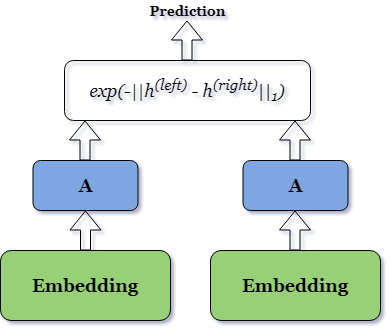
\includegraphics[scale=0.5]{figures/semantic_textual_similarity/siamese_neural_networks/siamese_architecture.png}
	\caption[Basic structure of the Siamese neural network]{Basic structure of the Siamese neural network. Unit A is changed over the architectures.}
	\label{fig:siamese}
\end{figure}


As the word embedding model, we used Word2vec embeddings \autocite{DBLP:journals/corr/abs-1301-3781} pre-trained on the Google news corpus\footnote{Pre-trained Word2vec can be downloaded from \url{https://code.google.com/archive/p/word2vec/}}. Using this model, we represented each word as a 300 length vector. For the words that do not appear in the model, we used a random vector. 
We evaluated all of the above variations in the three English STS datasets we introduced in \ref{cha:sts_introduction}; SICK, STS 2017 and QUORA. We trained the Siamese models on the training sets in these datasets and evaluated them on the testing sets. The results are shown in Table \ref{tab:sick_siamese}, Table \ref{tab:sts_siamese} and Table \ref{tab:quora_siamese} respectively.


\begin{table*}[htb]
	%\footnotesize
	\centering
	\scalebox{0.95}{
		\begin{tabular}{|l|cc|}
			\hline
			\textbf{Model} & $\bm{\rho}$   & $\bm{\tau}$     
			\\ \hline
			\textit{LSTM}                  
			& 0.802 & 0.733  \\
			\textit{Bi-LSTM}                     
			& 0.784 & 0.708   \\
			\textit{GRU}                     
			& 0.838$^{\dagger}$ & 0.780$^{\dagger}$  \\
			\textit{Bi-GRU}                     
			& 0.832 & 0.773  \\
			\textit{LSTM + Attention}                     
			& 0.827  & 0.765       \\
			\textit{GRU + Attention}                     
			& 0.818  & 0.751       \\
			\textit{GRU + Capsule + Flatten}                     
			& 0.806  & 0.733       \\
			\hline
		\end{tabular}
	}
	\caption[Results for SICK with Siamese Neural Network]{Results for SICK dataset with different variants of Siamese Neural Network. For each variant, Pearson Correlation ($\bm{\rho}$) and Spearman Correlation ($\bm{\tau}$) are reported between the predicted values and the gold labels of the test set. The best result from all the variations is marked with ${\dagger}$.}  
	\label{tab:sick_siamese}
\end{table*}


\begin{table*}[htb]
	%\footnotesize
	\centering
	\scalebox{0.95}{
		\begin{tabular}{|l|cc|}
			\hline
			\textbf{Model} & $\bm{\rho}$   & $\bm{\tau}$     
			\\ \hline
			\textit{LSTM}                  
			& 0.831 & 0.762  \\
			\textit{Bi-LSTM}                     
			& 0.784 & 0.708   \\
			\textit{GRU}                     
			& 0.853$^{\dagger}$ & 0.811$^{\dagger}$  \\
			\textit{Bi-GRU}                     
			& 0.844 & 0.804  \\
			\textit{LSTM + Attention}                     
			& 0.830  & 0.791       \\
			\textit{GRU + Attention}                     
			& 0.825  & 0.782       \\
			\textit{GRU + Capsule + Flatten}                     
			& 0.806  & 0.765       \\
			\hline
		\end{tabular}
	}
	\caption[Results for STS 2017 with Siamese Neural Network]{Results for STS 2017 dataset with different variants of Siamese Neural Network. For each variant, Pearson Correlation ($\bm{\rho}$) and Spearman Correlation ($\bm{\tau}$) are reported between the predicted values and the gold labels of the test set. The best result from all the variations is marked with ${\dagger}$. }  
	\label{tab:sts_siamese}
\end{table*}


\begin{table*}[htb]
	%\footnotesize
	\centering
	\scalebox{0.95}{
		\begin{tabular}{|l|c|}
			\hline
			\textbf{Model} & RMSE     
			\\ \hline
			\textit{LSTM}                  
			& 0.412   \\
			\textit{Bi-LSTM}                     
			& 0.402    \\
			\textit{GRU}                     
			& 0.415  \\
			\textit{Bi-GRU}                     
			& 0.408   \\
			\textit{LSTM + Attention}                     
			& 0.382$^{\dagger}$        \\
			\textit{GRU + Attention}                     
			& 0.398       \\
			\textit{GRU + Capsule + Flatten}                     
			& 0.421        \\
			\hline
		\end{tabular}
	}
	\caption[Results for QUORA with Siamese Neural Network]{Results for QUORA dataset with different variants of Siamese Neural Network. For each variant, Root Mean Squared Error (RMSE) reported between the predicted values and the gold labels of the test set. The best result from all the variations is marked with ${\dagger}$. }  
	\label{tab:quora_siamese}
\end{table*}

As can be seen in Tables \ref{tab:sick_siamese} and \ref{tab:sts_siamese}, for the SICK and STS2017 datasets, the GRU based Siamese neural network model outperformed the LSTM based Siamese neural network model, which we used as a baseline, and this provided the best result. It can be seen that complex architectures that involve Bi-directional RNNs, Attention and Capsule mechanisms did not perform well when compared to simple architectures like GRU. We can conclude that for the smaller datasets like STS 2017 and SICK, the GRU based architecture performs better because GRU has fewer parameters than LSTM \autocite{Chung2014EmpiricalEO}. With fewer parameters, the architecture does not need many training instances to optimise the weights during the training process.

However, when it comes to the big STS dataset, QUORA, the way the variants of the Siamese neural network behaves is different. As we introduced in Chapter \ref{cha:sts_introduction}, QUORA was the biggest STS dataset we experimented with, and it has 320,000 training instances. As a result, even complex architectures like RNNs with Attention get the opportunity to optimise their parameters and deliver good results. This can be seen in Table \ref{tab:quora_siamese}. For the QUORA dataset, the LSTM + Attention based Siamese neural network model outperformed the LSTM based Siamese neural network model, which we used as a baseline, and provided the best result. For bigger datasets, we can conclude that Siamese neural networks based on LSTM with Attention would outperform Siamese neural networks only with LSTMs. 

From the variants we examined, one notable observation is the poor performance of capsules in Siamese architectures. Despite providing good results in many NLP tasks such as text classification \autocite{NIPS2017_2cad8fa4,hettiarachchi-ranasinghe-2019-emoji, xia-etal-2018-zero, srivastava-etal-2018-identifying} and relation extraction \autocite{Zhang_Li_Jia_Zhao_2019, zhang-etal-2018-attention, 9095302}, the capsule-based variant failed to outperform the simple LSTM based variant even in the bigger STS dataset. This observation implies that capsule-based Siamese neural networks will not be a good fit for STS tasks.

With these findings, we answer our \textbf{RQ1} in this chapter. We have improved the state-of-the-art Siamese neural network architecture and propose a GRU based Siamese neural network architecture for the smaller STS datasets and LSTM + Attention based Siamese neural network for larger STS datasets.

\subsection{Impact of Transfer Learning}
\label{sec:siamese_transfer}
Transfer learning is a machine learning method where a model developed for a task is reused as the starting point for a model on a second task. It is a popular approach in deep learning where pre-trained models are used as the starting point for a new task. This is usually done in scenarios where there is not enough data to train a neural network, so that starting from already finetuned weights would be advantageous \autocite{pmlr-v97-houlsby19a, ruder-etal-2019-transfer}. Transfer learning has often provided good results for smaller datasets. Therefore, we explored the impact of transfer learning with Siamese neural networks in STS.

We saved the weights of the models that were trained on each STS dataset; SICK, STS 2017 and QUORA. We specifically used the two models that performed best in these datasets; Siamese neural network with GRU and the Siamese neural network with LSTM + Attention. We initiated training for each dataset, however rather than training from scratch, we used the weights of the models trained on another STS dataset. We compared these transfer learning results to the results we got from training the model from scratch. We conducted this transfer learning experiment only on the STS2017 and SICK datasets since the QUORA dataset is already large and transfer learning from a smaller dataset to a larger dataset is nonsensical.


\begin{table*}[htb]
	%\footnotesize
	\centering
	\scalebox{0.95}{
		\begin{tabular}{|l|c|c|}
			\hline
			\textbf{Start Model} & STS2017 & SICK      
			\\ \hline
			\textit{STS2017$_{GRU}$}                  
			& 0.853 & \textcolor{gray}{(+0.01)} \\
			\textit{STS2017$_{LSTM+Aten}$}                     
			& 0.830 & \textcolor{gray}{(+0.01)}  \\
			\hline
			\textit{SICK$_{GRU}$}                     
			& \textcolor{gray}{(+0.01)} & 0.838 \\
			\textit{SICK$_{LSTM+Aten}$}                     
			& \textcolor{gray}{(+0.01)} & 0.827 \\
			\hline
			\textit{QUORA$_{GRU}$}                     
			& \textcolor{gray}{(-0.02)}  &  \textcolor{gray}{(-0.02)}    \\
			\textit{QUORA$_{LSTM+Aten}$}                     
			& \textcolor{gray}{(-0.04)} &  \textcolor{gray}{(-0.04)}    \\
			\hline
		\end{tabular}
	}
	\caption[Results for transfer learning with Siamese Neural Network]{Results for transfer learning with different variants of Siamese Neural Network. For each transfer learning experiment we show the difference between with and without transfer learning. Non-grey values are the results of the experiments without transfer learning which we showed in the previous section. For ease of visualisation we only report the Pearson correlation ($\bm{\rho}$).}  
	\label{tab:transfer_siamese}
\end{table*}

As can be seen in Table \ref{tab:transfer_siamese} some of the transfer learning experiments improved the results for the STS2017 and SICK datasets with both architectures. The results improved when we performed transfer learning from STS2017 $\Rightarrow$ SICK and SICK $\Rightarrow$ STS2017. This shows that transfer learning can improve the results in Siamese neural networks. However, when we performed transfer learning from QUORA $\Rightarrow$ STS2017 and QUORA $\Rightarrow$ SICK, the results did not improve. In fact, they decrease, despite QUORA being the largest STS dataset we experimented with. This finding is somewhat controversial as the general belief in the community is that transfer learning from a larger dataset will improve the result. In this case, we believe that this happened because the QUORA dataset is very different to the other two datasets, as discussed in Chapter \ref{cha:sts_introduction}. Despite QUORA having a large number of training instances, when performing transfer learning, the neural network finds it difficult to optimise the weights for STS2017 and SICK as they were already optimised for a very different dataset; QUORA. This leads to a decrease in the results. On the other hand, transfer learning between STS2017 and SICK improved the results for both datasets since they are similar in nature, as we discussed in Chapter \ref{cha:sts_introduction}. 

Therefore, we can conclude that transfer learning can improve the results for Siamese neural networks in STS. However, the transfer learning dataset should be picked carefully taking the similarity of the two datasets into consideration, rather than only considering the size of the dataset.


\subsection{Impact of Data Augmentation}
\label{sec:siamese_aug}
As we observed earlier, the neural networks perform better when there are large number of training instances. Therefore, many approaches have been taken to increase the number of training instances. Usually, this has resulted in better performance with neural networks \autocite{wei-zou-2019-eda}. Therefore, we examined the impact of data augmentation on the Siamese neural network architectures proposed previously. We only conducted this experiment with the STS 2017 and SICK datasets as QUORA already has a large number of training instances.

We employed thesaurus-based augmentation in which 10,000 additional training examples are generated by replacing random words with one of their synonyms from Wordnet \autocite{10.1145/219717.219748}. A similar approach has also been successfully adapted by \textcite{Mueller_Thyagarajan_2016}, and \textcite{10.5555/2969239.2969312}.  We specifically used the two models that performed best with the bigger dataset and smaller dataset; Siamese neural network with GRU and Siamese neural network with LSTM + Attention. Since using transfer learning improved the results in the previous experiment, we trained the augmented training set on the transferred models; models trained on STS2017 for the SICK experiments and models trained on SICK for the STS2017 experiments. The results are shown in Table \ref{tab:augmentation_siamese}.  


\begin{table*}[htb]
	%\footnotesize
	\centering
	\scalebox{0.95}{
		\begin{tabular}{|c|c|c|}
			\hline
			\textbf{Dataset} &	\textbf{Start Model} &  $\bm{\rho}$      
			\\ \hline
			\multirow{ 2}{*}{\textit{SICK}}	& \textit{STS2017$_{GRU}$}                  
			& \textcolor{gray}{(+0.01)} \\
			&	\textit{STS2017$_{LSTM+Aten}$}                     
			& \textcolor{gray}{(+0.01)}  \\
			\hline
			\multirow{ 2}{*}{\textit{STS2017}}  & \textit{SICK$_{GRU}$}                     
			& \textcolor{gray}{(+0.01)}  \\
			& \textit{SICK$_{LSTM+Aten}$}                     
			& \textcolor{gray}{(+0.01)} \\
			\hline
		\end{tabular}
	}
	\caption[Results for data augmentation with Siamese Neural Networks]{Results for data augmentation with different variants of Siamese neural networks. For each data augmentation experiment, we show the difference between performing the data augmentation and without performing data augmentation. For ease of visualisation we only report the Pearson correlation ($\bm{\rho}$).} 
	\end{table*}
	
As can be seen in the Table \ref{tab:augmentation_siamese}, data augmentation improved the results of all the experiments. However, even with the additional 10,000 training instances, the GRU based Siamese neural network outperformed the LSTM + Attention based Siamese neural network. We can conclude that simple data augmentation techniques improve the performance of Siamese neural networks in STS tasks. From the Siamese neural network experiments we conducted, our best results for both the STS2017 and SICK datasets were provided by GRU based Siamese neural network when combined with transfer learning and data augmentation.
	
These observations answer our \textit{RQ2} in this Chapter; we can use transfer learning and simple data augmentation techniques to improve the results of Siamese neural networks in STS. 
	
	\begin{table*}[htb]
		%\footnotesize
		\centering
		\scalebox{0.95}{
			\begin{tabular}{|l|c|}
				\hline
				\textbf{Model} & $\bm{\rho}$      
				\\ \hline
				\cite{jimenez-etal-2014-unal} & 0.807 \\
				\cite{bjerva-etal-2014-meaning} & 0.827 \\
				\cite{zhao-etal-2014-ecnu-one} & 0.841 \\
				\textit{Siamese LSTM} & 0.863  \\
				\textit{Siamese GRU} & 0.882  \\
				\hline
			\end{tabular}
		}
		\caption[Results comparison for SICK with leader board results in SICK]{Results for SICK dataset with different variants of Siamese neural networks. For each variant, Pearson Correlation ($\bm{\rho}$) is reported between the predicted values and the gold labels of the test set.}  
		\label{tab:sick_siamese_all}
	\end{table*}
	
	\begin{table*}[htb]
		%\footnotesize
		\centering
		\scalebox{0.95}{
			\begin{tabular}{|l|c|}
				\hline
				\textbf{Model} & $\bm{\rho}$      
				\\ \hline
				\cite{tian-etal-2017-ecnu} & 0.851 \\
				\textit{Siamese LSTM} & 0.852  \\
				\cite{maharjan-etal-2017-dt} & 0.854 \\
				\cite{cer-etal-2017-semeval}  & 0.855   \\
				\textit{Siamese GRU} & 0.862  \\
				\hline
			\end{tabular}
		}
		\caption[Results comparison for STS2017 with leader board results in STS2017]{Results for STS2017 dataset with different variants of Siamese neural networks. For each variant, Pearson Correlation ($\bm{\rho}$) is reported between the predicted values and the gold labels of the test set.}  
		\label{tab:sts_siamese_all}
	\end{table*}
	
Furthermore, we compared the results of the best Siamese neural network variant with the best results submitted to the competitions \autocite{cer-etal-2017-semeval, marelli-etal-2014-semeval}, and with the unsupervised STS methods we have experimented with so far in the thesis. As can be seen in Tables \ref{tab:sick_siamese_all} and \ref{tab:sts_siamese_all}, the GRU based Siamese neural network architecture outperforms the best systems submitted to both competitions. It also outperforms the unsupervised STS methods we have explored so far in the thesis. Therefore, we can conclude that Siamese architecture is currently the best system we have experimented with for English STS.













\section{Portability to Other Languages}
\label{sec:siamese_languages}
Our \textit{RQ3} targets the multilingual aspect of the proposed approach; \textit{Can the proposed Siamese neural network be easily adopted into different languages?}. To answer this, we evaluated our method in the Arabic STS and Spanish STS datasets that were introduced in Chapter \ref{cha:sts_introduction}. Our approach has the advantage that it does not rely on language-dependent features.  As a result, the approach is easily portable to other languages, given the availability of pre-trained word embedding models in that particular language. The word embedding models, we used are AraVec \autocite{SOLIMAN2017256} \footnote{AraVec has been trained on Arabic Wikipedia articles. The models are available on \url{https://github.com/bakrianoo/aravec}} for Arabic and Spanish 3B words Word2Vec Embeddings \autocite{doi:10.1177/1550147718811827}\footnote{Spanish 3B words Word2Vec Embeddings have been trained on Spanish news articles, Wikipedia articles and Spanish Boletín Oficial del Estado (BOE; English: Official State Gazette). The model is available on \url{https://github.com/aitoralmeida/spanish_word2vec}} for Spanish.


\begin{table*}[htb]
	%\footnotesize
	\centering
	\scalebox{0.95}{
		\begin{tabular}{|l|cc|}
			\hline
			\textbf{Model} & $\bm{\rho}$   & $\bm{\tau}$     
			\\ \hline
			\textit{LSTM}                  
			& 0.746 & 0.690  \\
			\textit{Bi-LSTM}                     
			& 0.725 & 0.683   \\
			\textit{GRU}                     
			& 0.763$^{\dagger}$ & 0.723$^{\dagger}$  \\
			\textit{Bi-GRU}                     
			& 0.752 & 0.717  \\
			\textit{LSTM + Attention}                     
			& 0.741  & 0.703       \\
			\textit{GRU + Attention}                     
			& 0.739  & 0.691       \\
			\textit{GRU + Capsule + Flatten}                     
			& 0.712  & 0.679       \\
			\hline
		\end{tabular}
	}
	\caption[Results for Arabic STS with Siamese Neural Network]{Results for Arabic STS dataset with different variants of Siamese Neural Network. For each variant, Pearson Correlation ($\bm{\rho}$) and Spearman Correlation ($\bm{\tau}$) are reported between the predicted values and the gold labels of the test set. The best result from all the variations is marked with ${\dagger}$. }  
	\label{tab:arabic_siamese}
\end{table*}


\begin{table*}[htb]
	%\footnotesize
	\centering
	\scalebox{0.95}{
		\begin{tabular}{|l|cc|}
			\hline
			\textbf{Model} & $\bm{\rho}$   & $\bm{\tau}$     
			\\ \hline
			\textit{LSTM}                  
			& 0.842 & 0.773  \\
			\textit{Bi-LSTM}                     
			& 0.814 & 0.782   \\
			\textit{GRU}                     
			& 0.863$^{\dagger}$ & 0.822$^{\dagger}$  \\
			\textit{Bi-GRU}                     
			& 0.851 & 0.813  \\
			\textit{LSTM + Attention}                     
			& 0.845  & 0.801       \\
			\textit{GRU + Attention}                     
			& 0.832  & 0.790       \\
			\textit{GRU + Capsule + Flatten}                     
			& 0.795  & 0.773       \\
			\hline
		\end{tabular}
	}
	\caption[Results for Spanish STS with Siamese Neural Network]{Results for Spanish STS dataset with different variants of Siamese Neural Network. For each variant, Pearson Correlation ($\bm{\rho}$) and Spearman Correlation ($\bm{\tau}$) are reported between the predicted values and the gold labels of the test set. The best result from all the variations is marked with ${\dagger}$. }  
	\label{tab:spanish_siamese}
\end{table*}


As can be seen in Tables \ref{tab:arabic_siamese} and \ref{tab:spanish_siamese}, the GRU based Siamese neural network outperformed all other variants we experimented with in both Arabic and Spanish. As we discussed in Chapter \ref{cha:sts_introduction}, both of the Arabic and Spanish STS datasets we considered are small in size. Therefore, similarly to the STS2017 and SICK datasets, the GRU based Siamese neural network outperforms other architectures as GRU does not need a lot of training instances to optimise its weights. It should be noted that it is very easy to adapt this STS method in a different language. We only changed the embeddings to the new language and then performed the training. 

Furthermore, we compared the results of the best Siamese neural network variant with the best results submitted to the competition \autocite{cer-etal-2017-semeval}, and with the unsupervised STS methods we have experimented with so far in the thesis. 


\begin{table*}[htb]
	%\footnotesize
	\centering
	\scalebox{0.95}{
		\begin{tabular}{|l|c|}
			\hline
			\textbf{Model} & $\bm{\rho}$      
			\\ \hline
			\cite{tian-etal-2017-ecnu} & 0.744 \\
			\cite{nagoudi-etal-2017-lim} & 0.746 \\
			\textit{Siamese LSTM} & 0.746  \\
			\cite{wu-etal-2017-bit}  & 0.754   \\
			\textit{Siamese GRU} & 0.763  \\
			\hline
		\end{tabular}
	}
	\caption[Results comparison for Arabic STS with leader board results]{Results for Arabic STS dataset with different variants of Siamese Neural Network. For each variant, Pearson Correlation ($\bm{\rho}$) is reported between the predicted values and the gold labels of the test set.  }  
	\label{tab:arabic_siamese_all}
\end{table*}


\begin{table*}[htb]
	%\footnotesize
	\centering
	\scalebox{0.95}{
		\begin{tabular}{|l|c|}
			\hline
			\textbf{Model} & $\bm{\rho}$   \\  
			\hline
			\textit{Siamese LSTM} & 0.842  \\
			\cite{hassan-etal-2017-fcicu} & 0.848 \\
			\cite{wu-etal-2017-bit} &  0.850 \\
			\cite{tian-etal-2017-ecnu} & 0.855 \\
			\textit{Siamese GRU} & 0.863  \\
			\hline
		\end{tabular}
	}
	\caption[Results comparison for Spanish STS with leader board results]{Results for Spanish STS dataset with different variants of Siamese Neural Network. For each variant, Pearson Correlation ($\bm{\rho}$) is reported between the predicted values and the gold labels of the test set. }  
	\label{tab:spanish_siamese_all}
\end{table*}

As can be seen in Tables \ref{tab:arabic_siamese_all} and \ref{tab:spanish_siamese_all}, the Siamese neural network based on GRU outperforms the top three systems from the competition in both languages. Furthermore, it outperforms the unsupervised STS methods we have experimented with so far in the Thesis. Therefore, we can conclude that the Siamese neural network based on GRU is currently the best system we have experimented with for both Arabic and Spanish. 

These observations answer our \textbf{RQ3}; the Siamese architectures that we propose in this chapter can be successfully adapted in different languages by changing the word embeddings and the training dataset.

\section{Portability to Other Domains}
\label{sec:siamese_domains}
To answer our \textit{RQ4}; how well the proposed Siamese neural network architecture can be applied in different domains, we evaluated our method on the Bio-medical STS dataset explained in Chapter \ref{cha:sts_introduction} (BIOSSES). As we mentioned previously, the Bio-medical STS dataset does not have a training set. Therefore, we had to follow a transfer learning strategy to evaluate Siamese neural networks on the Bio-medical STS dataset. We used the pre-trained English STS models and performed inference on the Bio-medical STS dataset. We can refer to this as a \textit{"zero-shot transfer learning"} since the pre-trained English STS models did not see any Bio-medical data.

For this transfer learning strategy, we considered two word embedding models; the general Word2vec model we used before \cite{DBLP:journals/corr/abs-1301-3781} that was pre-trained on Google news corpus, and BioWordVec \cite{Zhang2019}, which has trained Word2vec on a combination of PubMed and PMC texts\footnote{The model is availble on \url{https://bio.nlplab.org/}}. With each word embedding model, we trained a Siamese neural network based on GRU and a Siamese neural network based on LSTM + Attention (the two best models we had from the English STS experiments) and evaluated them on the BIOSSES dataset.


\begin{table*}[htb]
	%\footnotesize
	\centering
	\scalebox{0.95}{
		\begin{tabular}{|c|c|c|c|}
			\hline
			\textbf{Data} &	\textbf{Model} & \textbf{Word2vec} & \textbf{BioWordVec}      
			\\ \hline
			\multirow{ 2}{*}{\textit{STS2017}}                  
			& \textit{Siamese GRU}	& 0.651 & 0.721 \\                  
			& \textit{Siamese LSTM+Atten} & 0.612 & 0.701  \\
			\hline
			\multirow{ 2}{*}{\textit{SICK}}                     
			& \textit{Siamese GRU}	& 0.642 & 0.719 \\                   
			& \textit{Siamese LSTM+Atten}	& 0.608 & 0.699 \\
			\hline
			\multirow{ 2}{*}{\textit{QUORA}}     &\textit{Siamese GRU}                     
			& 0.591  &  0.622    \\
			&	\textit{Siamese LSTM+Atten}                     
			& 0.603 &  0.634   \\
			\hline
		\end{tabular}
	}
	\caption[Results for transfer learning with Siamese Neural Network in BIOSSES dataset]{Results for transfer learning with different variants of Siamese neural networks in BIOSSES dataset. \textbf{Data} column shows the datasets we performed transfer learning from and \textbf{Model} column displays the Siamese variant we employed. Two considered word embedding models are \textbf{Word2vec} and \textbf{BioWordVec}. For ease of visualisation we only report the Pearson correlation ($\bm{\rho}$).}  
	\label{tab:transfer_siamese_biosses}
\end{table*}

As you can see in Table \ref{tab:transfer_siamese_biosses}, Siamese neural architectures provided satisfactory results. We got the best result from the Siamese neural network based on GRU, when trained on STS 2017 using BioWordVec. However, the results from the SICK dataset are not far behind. There was a clear improvement when the English STS model was trained using BioWordVec rather than general Word2vec embeddings. This may be because most of the Bio-medical words that appear in the BIOSSES dataset are out of vocabulary in general Word2vec embeddings, which can cause problems for the neural network when it observes them in the testing phase. It should be noted that in this experiment, when we performed transfer learning from the QUORA dataset, the results are lower than when we performed transfer learning from SICK or STS 2017. This again may be due to the fact that the SICK and STS2017 datasets have a similar annotation strategy to the BIOSSES dataset as discussed in Chapter \ref{cha:sts_introduction}. Even though QUORA has a large number of training instances, it can't produce good transfer learning results because its annotation strategy is different. 



\begin{table}[htb]
	%\footnotesize
	\centering
	\scalebox{0.95}{
		\begin{tabular}{|l|c|}
			\hline
			\textbf{Model} & $\bm{\rho}$   \\  
			\hline
			\textit{ELMo $\bigoplus$ BERT}  &  0.708 \\
			\textit{Siamese GRU$_{STS2017}$} & 0.719 \\
			\cite{10.1093/bioinformatics/btx238} & 0.754 \\
			\textit{BioSentVec} \cite{8904728} & 0.810  \\
			\hline
		\end{tabular}
	}
	\caption[Results comparison for BIOSSES with top results]{Results for BIOSSES dataset with different variants of Siamese Neural Network compared with top results reported for BIOSSES. For each variant, Pearson Correlation ($\bm{\rho}$) is reported between the predicted values and the gold labels of the test set. }  
	\label{tab:biosses_siamese_all}
\end{table}


Furthermore, we compared our results with the best results reported for the dataset. The results are shown in Table \ref{tab:biosses_siamese_all}. The best model we had in Table \ref{tab:transfer_siamese_biosses} which is the Siamese GRU model trained on the STS2017 dataset, is represented as \textit{Siamese GRU$_{STS2017}$}. As shown in Table \ref{tab:biosses_siamese_all}, our method provides satisfactory results compared with the best approaches submitted to the BIOESS dataset. However, the unsupervised method we experimented with in the previous chapter with BioSentVec \autocite{8904728}, comfortably outperformed the Siamese neural network approaches we explored in this chapter. We can answer our \textbf{RQ4}: \textit{How well does the proposed Siamese neural network perform in a different domain?} with these findings. The Siamese neural network architectures can be adapted to different domains by changing the pre-trained word embeddings. However, without a proper training set, the results are not strong. 

\section{Conclusions}
\label{sec:siamese_conclusions}
This chapter experimented with using Siamese neural networks for calculating semantic similarity between pairs of texts and compared them with other unsupervised/ supervised approaches. We used an existing Siamese neural network as the baseline; MALSTM \autocite{Mueller_Thyagarajan_2016} and explored six different variants of Siamese neural networks. We experimented with three English STS datasets, SICK, STS2017 and QUORA. For the smaller STS datasets; SICK and STS2017, we show that the Siamese neural network based on GRU outperforms the baseline. For the larger STS dataset; QUORA, we show that Siamese neural network with LSTM and Attention outperforms the baseline. Also, we show that we can further improve the results with transfer learning and data augmentation techniques. However, we experienced that performing transfer learning from a bigger dataset does not always improve the results. The quality of the dataset which was used for transfer learning also matters. We show that Siamese neural network based on GRU outperforms the top submissions in both \textit{SemEval 2017 task 1} \autocite{cer-etal-2017-semeval} and  \textit{SemEval 2014 task 1} \autocite{marelli-etal-2014-semeval}. The data augmentation techniques we used in this chapter are language-dependent as they rely on WordNet \autocite{10.1145/219717.219748}. However, as future work, we can experiment with data augmentation techniques that are not language dependant and relies on word embeddings \autocite{kumar-etal-2020-data}. 

We extended the experiments with the Siamese neural network architectures to the Arabic and Spanish STS datasets \autocite{cer-etal-2017-semeval}. In these experiments, the GRU based Siamese neural network architecture again outperformed all the systems submitted to the shared task and outperformed all of the STS methods we have experimented with so far in this part of the thesis. This proves that the Siamese neural network that we propose in this study, can be adapted to different languages. Furthermore, we performed experiments with the BIOSSES dataset. However, since the BIOSSES dataset does not have a training set, we used transfer learning based zero-shot learning when Siamese neural networks are applied. Even though they provided satisfactory results, Siamese neural networks could not outperform the sentence encoder based method we explored in Chapter \ref{cha:sts_sentence_encoders}. We can conclude that even though the Siamese neural networks can be adapted into different domains by changing the word embedding model, they do not provide strong results without a proper training set. 

Since word embedding models are now available in most languages, including low resource languages such as Urdu \autocite{haider-2018-urdu}, Telugu \autocite{kumar-etal-2020-passage} and domains such as the legal domain \autocite{Chalkidis2019}, the method we experimented with in this chapter can be useful for many languages and domains. However, one drawback is the need for STS training data in each language and domain, this can be challenging in many scenarios. 

As future work, it would be interesting to experiment transfer learning between languages with cross-lingual embeddings such as fastText \autocite{mikolov-etal-2018-advances} using Siamese neural networks. Such an approache will train an STS model on resource-rich languages like English and project the prediction for other languages using the zero-shot transfer learning. It would be a potential solution to satisfy the training data requirement for low resource languages. 

With the introduction of transformer models such as BERT \autocite{devlin-etal-2019-bert} and XLNet \autocite{yang2019xlnet}, Siamese neural networks have evolved by utilising transformers in their architectures \autocite{reimers-gurevych-2019-sentence}. We will discuss these further in Chapter \ref{cha:sts_transformers}. 












\chapter{\label{cha:sts_transformers}Adapting Transformers for STS}

Transformers can be considered as the most significant revolution that happened in NLP in recent years. Similarly to Recurrent Neural Networks (RNNs), transformers handle sequential input data, such as natural language, for tasks including machine translation and text summarisation. However, unlike RNNs, transformers do not necessarily process the sequences in order. Instead, the attention mechanism in transformers handles the context for any position in the input sequence. For example, if the input data is a sentence, the transformer does not need to process the beginning of the sentence before the end. Since RNNs process the sequence in order, they often forget the content of distant positions in the sequence. This nature of the RNNs causes problems when processing long sequences. Furthermore, since RNNs process word by word, it is hard to parallelise the work for processing sentences. The attention mechanism in transformers can address both of these issues \autocite{NIPS2017_3f5ee243}.


Transformers were first introduced in \textcite{NIPS2017_3f5ee243}, where the authors used a transformer architecture for the sequence to sequence tasks such as machine translation. They show that an architecture with only attention mechanisms and without any RNNs can improve the results in the sequence to sequence tasks. The first notable research in using transformers for language modelling was OpenAI GPT \autocite{radford2018improving}. OpenAI GPT adapts a pre-training followed by a fine-tuning scheme which means that once pre-trained, it can be fine-tuned to a large number of downstream NLP tasks such as text classification, named entity recognition etc. However, the first breakthrough in using transformer models for language modelling happened with the introduction of BERT \autocite{devlin-etal-2019-bert}. As we explain in Section \ref{sec:transformers_related}, BERT employs a masked language modelling (MLM) objective, which brings improvements over OpenAI GPT. Later, different variants of BERT were proposed by the NLP community. We explain some of these models that we used in this chapter in Section \ref{sec:transformers_related}. All of these transformer models follow the same fine-tuning scheme of BERT.


Transformer models, which we have experimented with in this chapter, use special tokens to obtain a single contiguous sequence for each input sequence. Specifically, the first token is always a special classification token (\textsc{[CLS]}), and sentence pairs are separated using a special token (\textsc{[SEP]}). The final hidden state of \textsc{[CLS]}  is used for the sentence-level fine-tuning tasks such as text classification \autocite{10.1007/978-3-030-32381-3_16, ranasinghe-hettiarachchi-2020-brums}, and the final hidden state of each token is used for the token-level fine-tuning tasks such as named entity recognition \autocite{taher-etal-2019-beheshti, ranasinghe-etal-2021-wlv,jia-etal-2020-entity}. The fine-tuning scheme in transformers is usually simple. For example, transformer models can be adapted to text classification tasks by adding a softmax layer on top of \textsc{[CLS]} token. Furthermore, the fine-tuning scheme is very efficient as the parameters in the transformer model are already optimised in the pre-training process. Therefore, transformer models have been prevalent and successful in many NLP tasks \autocite{devlin-etal-2019-bert}. 

In this chapter, we experiment with different transformers models in a variety of STS datasets. 
We address four research questions in this chapter:

\textbf{RQ1:} How well do the existing state-of-the-art transformer models perform in the STS task? 

\textbf{RQ2:} Can the method improve with the transfer learning and data augmentation techniques?

\textbf{RQ3:} Can the transformer model be easily adapted to different languages?

\textbf{RQ4:} How well do the proposed transformer models perform in a different domain? 

The main contributions of this chapter are as follows.

\begin{enumerate}
\item We evaluate five popular transformer models in three English STS datasets. We compare the results with the previous STS methods and show that transformer-based STS methods outperform all the other STS methods we have experimented with in this thesis.

\item We propose further enhancements to the architecture using transfer learning and data augmentation.   

\item We evaluate how well the transformer models perform on STS datasets in different languages and domains. 

\item The code and the pre-trained models are publicly available to the community\footnote{The public GitHub repository is available on \url{https://github.com/tharindudr/STS-Transformers}.}. We have published the code as a Python library \footnote{The developed python library is available on \url{https://pypi.org/project/ststransformers/}.} and by the time of writing this chapter, it has more than 3,000 downloads from the community. 

\end{enumerate}

The rest of this chapter is organised as follows. Section \ref{sec:transformers_related} describes the pre-trained transformer models used in this chapter. Section \ref{sec:transformer_method} discusses the architecture and \ref{sec:transformer_english} shows the experiments conducted with three English STS datasets. Sections \ref{sec:transformer_transfer} and \ref{sec:transformer_aug} provide more experiments to improve the results. Experiments done with other languages and domains are shown in Sections \ref{sec:transformer_multilingual} and \ref{sec:transformer_domain}. Section \ref{sec:transformer_siamese} discusses the recent developments carried out with integrating transformers into Siamese architectures, addressing a key issue in using transformers in STS. The chapter finishes with conclusions and ideas for future research directions in transformers. 

\section{Related Work}
\label{sec:transformers_related}
As we mentioned before, after the introduction of BERT \autocite{devlin-etal-2019-bert}, many variants of different transformer models have been proposed by adding minor modifications to the original BERT transformer. Usually, these modifications have resulted in improvements in the fine-tuning scheme for the downstream NLP tasks. Expecting a similar behaviour for the STS task, we evaluated the following transformer models for the experiments in this chapter.

\paragraph{BERT} \autocite{devlin-etal-2019-bert} proposes an MLM objective, where some of the tokens of the input sequence are randomly masked, and the objective is to predict these masked positions, taking the corrupted sequence as input. BERT applies a Transformer encoder to attend to bi-directional contexts during pre-training. In addition, BERT uses a next-sentence-prediction (NSP) objective. Given two input sentences, NSP predicts whether the second sentence is the next sentence of the first sentence. The NSP objective aims to improve the tasks which require reasoning over sentence pairs, such as question answering and natural language inference. 

\paragraph{RoBERTa} \autocite{liu2019roberta} makes a few changes to the BERT architecture and achieves substantial improvements. These changes include: (1) Training the model longer with larger batches and more data; (2) Removing the NSP objective; (3) Training on longer sequences; (4) Dynamically changing the masked positions during pre-training. The authors show that these changes lead to significant improvements in the downstream NLP tasks.

\paragraph{ALBERT} \autocite{Lan2020ALBERT} proposes two parameter-reduction techniques (factorised embedding parameterisation and cross-layer parameter sharing) to lower memory consumption and speed up training. Furthermore, ALBERT \autocite{Lan2020ALBERT} shows that the NSP objective in BERT lacks difficulty, as the negative examples are created by pairing segments from different documents, which mixes topic prediction and coherence prediction into a single task. Instead of that, ALBERT uses a sentence-order prediction (SOP) objective. SOP obtains positive examples by taking out two consecutive segments and negative examples by reversing the order of two consecutive segments from the same document. The results show that ALBERT provides better results than BERT in many downstream NLP tasks.


\paragraph{ELECTRA} Compared to BERT, ELECTRA \autocite{Clark2020ELECTRA} proposes an effective pre-training method. Instead of corrupting some positions of inputs with [MASK], ELECTRA replaces some tokens of the inputs with their plausible alternatives sampled from a small generator network. ELECTRA trains a discriminator to predict whether the generator replaced each token in the corrupted input or not. The pre-trained discriminator can then be used in downstream tasks for fine-tuning, improving upon the pre-trained representation learned by the generator.ed in downstream tasks for fine-tuning, improving upon the pre-trained representation learned by the generator.

\paragraph{XLNET} \autocite{yang2019xlnet} addresses a key weakness in BERT pre-training. \textcite{yang2019xlnet} show that the symbols such as \textsc{[MASK]} that BERT introduces during pre-training cause a discrepancy between pre-training and fine-tuning as they never occur in real data. Therefore, XLNET proposes a new auto-regressive method based on permutation language modelling (PLM) \autocite{JMLR:v17:16-272} without introducing new symbols. 

Upon the introduction, these transformer models are evaluated in many downstream NLP tasks, including STS. However, there is no comprehensive study on STS using the transformers in large and small STS datasets, transfer learning, data augmentation, multilingual STS, etc., which we do in this chapter.

\section{Transformer Architecture for STS}
\label{sec:transformer_method}

\begin{figure}[ht]
	\centering
	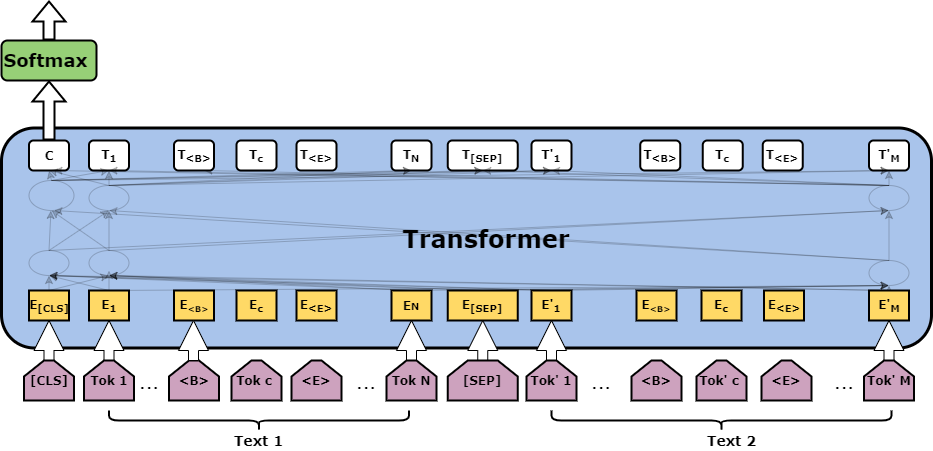
\includegraphics[scale=0.4]{figures/semantic_textual_similarity/transformers/STSTransformers.png}
	\caption[Architecture for using Transformers in STS]{Architecture for using Transformers in STS.}
	\label{fig:sts_transformers}
\end{figure}

The transformer architecture for STS is shown in Figure \ref{fig:sts_transformers}. The input of this model is a concatenation of the two sentences, separated by the \textsc{[SEP]} token. Then the output of the \textsc{[CLS]} token is used as the input of a softmax layer that predicts the similarity of the two sentences. We used the mean-squared-error loss as the objective function. For the configurations, we used a batch-size of eight, Adam optimiser with a learning rate $2\mathrm{e}^{-5}$, and a linear learning rate warm-up over 10\% of the training data. During the training process, the parameters of the transformer and the parameters of the subsequent layers were updated. The models were trained using only training data. Furthermore, they were evaluated while training after every 100 batches, using an evaluation set that had one-fifth of the instances in training data. We performed early stopping if the evaluation loss did not improve over ten evaluation steps. All the models were trained for three epochs. As these transformer models are computationally expensive, we used an Nvidia Tesla T4 GPU for the training process. We have kept these configurations the same for all the experiments to ensure consistency between all the experiments. The implementation is based on PyTorch \autocite{NEURIPS2019_9015} and HuggingFace \autocite{wolf-etal-2020-transformers}.


\section{Exploring Transformers in English STS}
\label{sec:transformer_english}
We evaluated all the transformer variations mentioned before, in three English STS datasets we introduced in \ref{cha:sts_introduction}; SICK, STS 2017 and QUORA. All of the transformer models we experimented have several models that supports English (e.g.\ \textit{bert-large-cased} \& \textit{bert-base-cased} for BERT, \textit{albert-xxlarge-v2} \& \textit{albert-base-v2} for ALBERT), and usually the large models outperform the smaller models in downstream tasks. Therefore, we used the largest possible model that our GPU setup can load with each transformer type; \textit{bert-large-cased} for BERT \autocite{devlin-etal-2019-bert}, \textit{albert-large-v2} for ALBERT \autocite{Lan2020ALBERT}, \textit{roberta-large} for RoBERTa \autocite{liu2019roberta}, \textit{google/electra-large-discriminator} for ELECTRA \autocite{Clark2020ELECTRA} and \textit{xlnet-large-cased}  \autocite{yang2019xlnet} for XLNET. All of these models are available in HuggingFace \autocite{wolf-etal-2020-transformers} model hub\footnote{Models are available on \url{https://huggingface.co/models}}.

We trained the transformer models on the training sets of these datasets and evaluated on the testing sets. The results for the SICK, STS2017 and QUORA are shown in Tables \ref{tab:sick_transformers}, \ref{tab:sts_transformers} and \ref{tab:quora_transformers}, respectively. 

\begin{table*}[htb]
	%\footnotesize
	\centering
	\scalebox{0.95}{
		\begin{tabular}{|l|cc|}
			\hline
			\textbf{Model} & $\bm{\rho}$   & $\bm{\tau}$     
			\\ \hline
			\textit{BERT}                  
			& 0.881 & 0.826  \\
			\textit{ALBERT}                  
			& 0.886 & 0.829  \\
			\textit{RoBERTa}                  
			& 0.892$^{\dagger}$ & 0.834$^{\dagger}$  \\
			\textit{ELECTRA}                  
			& 0.872 & 0.819  \\
			\textit{XLNET}                  
			& 0.879 & 0.821  \\
			\hline
		\end{tabular}
	}
	\caption[Results for SICK with Transformer Models]{Results for SICK dataset with different variants of transformer models. For each variant, Pearson Correlation ($\bm{\rho}$) and Spearman Correlation ($\bm{\tau}$) are reported between the predicted values and the gold labels of the test set. The best result from all of the variations is marked with ${\dagger}$.}  
	\label{tab:sick_transformers}
\end{table*}


\begin{table*}[htb]
	%\footnotesize
	\centering
	\scalebox{0.95}{
		\begin{tabular}{|l|cc|}
			\hline
			\textbf{Model} & $\bm{\rho}$   & $\bm{\tau}$     
			\\ \hline
				\textit{BERT}                  
		& 0.889 & 0.858  \\
		\textit{ALBERT}                  
		& 0.874 & 0.852  \\
		\textit{RoBERTa}                  
		& 0.895$^{\dagger}$ & 0.861$^{\dagger}$  \\
		\textit{ELECTRA}                  
		& 0.873 & 0.849  \\
		\textit{XLNET}                  
		& 0.868 & 0.843  \\
			\hline
		\end{tabular}
	}
	\caption[Results for STS 2017 with Transformers]{Results for STS 2017 dataset with different variants of Transformers. For each variant, Pearson Correlation ($\bm{\rho}$) and Spearman Correlation ($\bm{\tau}$) are reported between the predicted values and the gold labels of the test set. The best result from all of the variations is marked with ${\dagger}$. }  
	\label{tab:sts_transformers}
\end{table*}


\begin{table*}[htb]
	%\footnotesize
	\centering
	\scalebox{0.95}{
		\begin{tabular}{|l|c|}
			\hline
			\textbf{Model} & RMSE     
			\\ \hline
			\textit{BERT}                  
			& 0.349   \\
			\textit{ALBERT}                  
			& 0.354   \\
			\textit{RoBERTa}                  
			& 0.359   \\
			\textit{ELECTRA}                  
			& 0.353   \\
			\textit{XLNET}                  
			& 0.346$^{\dagger}$   \\
			\hline
		\end{tabular}
	}
	\caption[Results for QUORA with Transformers]{Results for QUORA dataset with different variants of Transformers. For each variant, Root Mean Squared Error (RMSE) reported between the predicted values and the gold labels of the test set. The best result from all of the variations is marked with ${\dagger}$. }  
	\label{tab:quora_transformers}
\end{table*}

As can be seen in Tables \ref{tab:sick_transformers} and \ref{tab:sts_transformers}, for the SICK and STS 2017 datasets, RoBERTa outperformed other transformer models. Since SICK and STS 2017 are smaller datasets, the optimised nature of RoBERTa is beneficial. The QUORA dataset, which is larger than the SICK and STS 2017, \textit{XLNET}  outperforms other transformer models. However, from the results, there is no clear indication of which transformer model would perform best in a particular dataset other than the fact that the \textit{RoBERTa} performs slightly better in smaller datasets. It should be noted that all of the transformers perform on par with each other. 

In the initial experiments, we noticed that the transformer models are susceptible to the random seed\footnote{A random seed is used to configure the starting weights in a neural network. Keeping the random seed constant in the experiments removes the variation due to this randomness, making it easier to interpret the effects of other design changes such as hyperparameter values.} of the experiments \autocite{zhang2021revisiting}. Changing the random seed led to different results. To minimise this effect from the random seed, we conducted experiments for five different random seeds. We took the mean of these experiments as the final results, which is the value reported in Tables \ref{tab:sick_transformers}, \ref{tab:sts_transformers} and \ref{tab:quora_transformers}. We noticed that doing many experiments with different random seeds reduced the variance of the final result. 

With this, we answer our \textbf{RQ1}: transformers can be successfully adapted in the STS task, and they produce good results in all the datasets. For the smaller datasets, \textit{RoBERTa} performed slightly better than other transformer models. Furthermore, we recommend conducting more experiments with different random seeds to minimise the variance.


\subsection{Impact of Transfer Learning}
\label{sec:transformer_transfer}
Similar to the \textit{Siamese neural networks} in Chapter \ref{cha:sts_siamese_neural_networks}, we explored the impact of transfer learning  in STS, with transformers. We saved the weights of the transformers models trained on each STS dataset; SICK, STS 2017 and QUORA. We specifically used the two models that performed best in these datasets; RoBERTa and XLNET. We again initiated training for each dataset; however, rather than training the transformer models from scratch, we used the weights of the models trained on a different STS dataset. We compared these transfer learning results to the results we got from training the model from scratch. Similar to the \textit{Siamese neural network} experiments, we conducted this transfer learning experiment only on the STS2017 and SICK datasets since the QUORA dataset is already large and transfer learning from a smaller dataset to a larger dataset is nonsensical.


\begin{table*}[htb]
	%\footnotesize
	\centering
	\scalebox{0.95}{
		\begin{tabular}{|l|c|c|}
			\hline
			\textbf{Start Model} & STS2017 & SICK      
			\\ \hline
			\textit{STS2017$_{RoBERTa}$}                  
			& 0.895 & \textcolor{gray}{(+0.009)} \\
			\textit{STS2017$_{XLNET}$}                     
			& 0.868 & \textcolor{gray}{(+0.011)}  \\
			\hline
			\textit{SICK$_{RoBERTa}$}                     
			& \textcolor{gray}{(+0.008)} & 0.892 \\
			\textit{SICK$_{XLNET}$}                     
			& \textcolor{gray}{(+0.013)} & 0.879 \\
			\hline
			\textit{QUORA$_{RoBERTa}$}                     
			& \textcolor{gray}{(-0.025)}  &  \textcolor{gray}{(-0.021)}    \\
			\textit{QUORA$_{XLNET}$}                     
			& \textcolor{gray}{(-0.039)} &  \textcolor{gray}{(-0.043)}    \\
			\hline
		\end{tabular}
	}
	\caption[Results for transfer learning with Transformers]{Results for transfer learning with different Transformers. For each transfer learning experiment we show the difference between with and without transfer learning. Non-grey values are the results of the experiments without transfer learning which we showed in the previous section. For ease of visualisation we only report the Pearson correlation ($\bm{\rho}$).}  
	\label{tab:transfer_transformers}
\end{table*}

As can be seen in Table \ref{tab:transfer_transformers}, when we performed transfer learning from STS2017 $\Rightarrow$ SICK and SICK $\Rightarrow$ STS2017 the results improve. This shows that transfer learning can improve the results of transformers. However, similar to the \textit{Siamese neural networks}, when we performed transfer learning from QUORA $\Rightarrow$ STS2017 and QUORA $\Rightarrow$ SICK, the results did not improve, in fact, they decrease. Therefore, we can assume that performing transfer learning from a very different dataset, is not beneficial in transformers. 

Therefore, we can conclude that transfer learning can improve the results for transformers in STS. However, the transfer learning dataset should be picked carefully, taking the similarity of the two datasets into consideration, rather than only considering the size of the dataset.


\subsection{Impact of Data Augmentation}
\label{sec:transformer_aug}
Since the transformer models have provided better results with more training data, we experimented with the impact of data augmentation on the transformer models. Similar to the \textit{Siamese neural networks} in Chapter \ref{cha:sts_siamese_neural_networks}, we employed thesaurus-based augmentation in which 10,000 additional training examples are generated by replacing random words with one of their synonyms in Wordnet \autocite{10.1145/219717.219748}. We specifically used the two models that performed best with the bigger dataset and smaller dataset; \textit{RoBERTa} and \textit{XLNET}. Since using transfer learning improved the results in the previous experiment, we trained the augmented training set on the transferred models; models trained on STS2017 for the SICK experiments and models trained on SICK for the STS2017 experiments. The results are shown in Table \ref{tab:augmentation_transformers}. 

\begin{table*}[htb]
	%\footnotesize
	\centering
	\scalebox{0.95}{
		\begin{tabular}{|c|c|c|}
			\hline
			\textbf{Dataset} &	\textbf{Start Model} &  $\bm{\rho}$      
			\\ \hline
			\multirow{ 2}{*}{\textit{SICK}}	& \textit{STS2017$_{RoBERTa}$}                  
			& \textcolor{gray}{(+0.012)} \\
			&	\textit{STS2017$_{XLNET}$}                     
			& \textcolor{gray}{(+0.011)}  \\
			\hline
			\multirow{ 2}{*}{\textit{STS2017}}  & \textit{SICK$_{RoBERTa}$}                     
			& \textcolor{gray}{(+0.014)}  \\
			& \textit{SICK$_{XLNET}$}                     
			& \textcolor{gray}{(+0.013)} \\
			\hline
		\end{tabular}
	}
	\caption[Results for data augmentation with Transformers]{Results for data augmentation with different transformers. For each data augmentation experiment we show the difference between with dat augmentation and without data augmentation. For ease of visualisation we only report the Pearson correlation ($\bm{\rho}$).}  
	\label{tab:augmentation_transformers}
\end{table*}

As can be seen in Table \ref{tab:augmentation_transformers}, data augmentation improved the results of all the experiments with transformers. However, even with the additional 10,000 training instances, \textit{RoBERTa} outperformed \textit{XLNET}. We can conclude that simple data augmentation techniques can improve the performance of transformers in the STS task. From the experiments we conducted, our best results for both the STS2017 and SICK datasets were produced by \textit{RoBERTa} when combined with transfer learning and data augmentation.


These observations answer our \textit{RQ2} in this Chapter; we can use transfer learning and simple data augmentation techniques to improve the results of transformers in STS. 

\begin{table*}[htb]
	%\footnotesize
	\centering
	\scalebox{0.95}{
		\begin{tabular}{|l|c|}
			\hline
			\textbf{Model} & $\bm{\rho}$      
			\\ \hline
			\textcite{jimenez-etal-2014-unal} & 0.807 \\
			\textcite{bjerva-etal-2014-meaning} & 0.827 \\
			\textcite{zhao-etal-2014-ecnu-one} & 0.841 \\
			\textit{Siamese GRU} & 0.882  \\
			\textit{RoBERTa} & 0.920  \\
			\hline
		\end{tabular}
	}
	\caption[Results comparison for SICK with leader board results including transformers]{Results for the SICK dataset with different transformer models. For each variant, Pearson Correlation ($\bm{\rho}$) is reported between the predicted values and the gold labels of the test set.}  
	\label{tab:sick_transformers_all}
\end{table*}

\begin{table*}[htb]
	%\footnotesize
	\centering
	\scalebox{0.95}{
		\begin{tabular}{|l|c|}
			\hline
			\textbf{Model} & $\bm{\rho}$      
			\\ \hline
			\textcite{tian-etal-2017-ecnu} & 0.851 \\
			\textcite{maharjan-etal-2017-dt} & 0.854 \\
			\textcite{cer-etal-2017-semeval}  & 0.855   \\
			\textit{Siamese GRU} & 0.862  \\
			\textit{RoBERTa} & 0.915  \\
			\hline
		\end{tabular}
	}
	\caption[Results comparison for STS2017 with leader board results]{Results for the STS2017 dataset with different variants of Siamese Neural Network. For each variant, Pearson Correlation ($\bm{\rho}$) is reported between the predicted values and the gold labels of the test set.  }  
	\label{tab:sts_transformers_all}
\end{table*}

Furthermore, we compared the results of the best transformer model with the best results submitted to the competitions \autocite{cer-etal-2017-semeval, marelli-etal-2014-semeval}, and with the supervised and unsupervised STS methods, we have experimented in this thesis. As can be seen in Tables \ref{tab:sick_transformers_all} and \ref{tab:sts_transformers_all}, \textit{RoBERTa} outperforms the best system submitted to both competitions. It also outperforms the unsupervised and supervised STS methods we have explored in this thesis, including \textit{Siamese neural networks}. Therefore, we can conclude that transformers are the current state-of-the-art for English STS.

\section{Portability to Other Languages}
\label{sec:transformer_multilingual}
Similar to the other STS methods we have experimented with in this thesis, we evaluated transformers in Arabic STS and Spanish STS datasets introduced in Chapter \ref{cha:sts_introduction}. Transformers have the advantage that they do not rely on language-dependent features.  As a result, the approach is easily portable to other languages, given the availability of the pre-trained transformer models in that particular language. The transformer models, we used are AraBERT and AraELECTRA for Arabic which were trained on Arabic Wikipedia dump, the 1.5B words Arabic Corpus \autocite{elkhair201615}, the OSCAR corpus \autocite{ortiz-suarez-etal-2020-monolingual} and the OSIAN Corpus \autocite{zeroual-etal-2019-osian} using original BERT and ELECTRA architectures explained in Section \ref{sec:transformers_related}\footnote{More details about the models and download links are available on \url{https://github.com/aub-mind/arabert}}. Both of these models use Farasa segmentation as a pre-processing step \autocite{abdelali-etal-2016-farasa}. For Spanish, we used BETO; a Spanish BERT model \autocite{CaneteCFP2020} trained on Spanish Unannotated Corpora\footnote{Corpora is available on \url{https://github.com/josecannete/spanish-corpora}} using the original BERT architecture\footnote{More details about BETO is available on \url{https://github.com/dccuchile/beto}}. Additionally, for both languages, we used the "BERT-Base, Multilingual Cased" model \autocite{devlin-etal-2019-bert}, which is trained on the top 100 languages with the largest Wikipedias that includes Arabic and Spanish languages.

The results are shown in Tables \ref{tab:arabic_transformers_all} and \ref{tab:spanish_transformers_all} for the Arabic and Spanish datasets. We also compared the results of the transformer models with the best methods submitted to the competition \autocite{cer-etal-2017-semeval}, and with the supervised/unsupervised STS methods, we have experimented in this thesis. 


\begin{table*}[htb]
	%\footnotesize
	\centering
	\scalebox{0.95}{
		\begin{tabular}{|l|c|}
			\hline
			\textbf{Model} & $\bm{\rho}$      
			\\ \hline
			\textcite{tian-etal-2017-ecnu} & 0.744 \\
			\textcite{nagoudi-etal-2017-lim} & 0.746 \\
			\textcite{wu-etal-2017-bit}  & 0.754   \\
			\textit{Siamese GRU} & 0.763  \\
			\textit{mBERT} & 0.778\\
			\textit{AraElectra} & 0.791\\
			\textit{AraBERT} & \textbf{0.794} \\
			\hline
		\end{tabular}
	}
	\caption[Results comparison for Arabic STS with leader board results]{Results for the Arabic STS dataset with different transformers. For each variant, Pearson Correlation ($\bm{\rho}$) is reported between the predicted values and the gold labels of the test set. }  
	\label{tab:arabic_transformers_all}
\end{table*}


\begin{table*}[htb]
	%\footnotesize
	\centering
	\scalebox{0.95}{
		\begin{tabular}{|l|c|}
			\hline
			\textbf{Model} & $\bm{\rho}$   \\  
			\hline
			\textcite{hassan-etal-2017-fcicu} & 0.848 \\
			\textcite{wu-etal-2017-bit} &  0.850 \\
			\textcite{tian-etal-2017-ecnu} & 0.855 \\
			\textit{Siamese GRU} & 0.863  \\
			\textit{mBERT} & 0.884  \\
			\textit{BETO} & \textbf{0.890}  \\
			\hline
		\end{tabular}
	}
	\caption[Results comparison for Spanish STS with leader board results]{Results for the Spanish STS dataset with different variants of Siamese Neural Network. For each variant, Pearson Correlation ($\bm{\rho}$) is reported between the predicted values and the gold labels of the test set. }  
	\label{tab:spanish_transformers_all}
\end{table*}

As can be seen in the results transformer based STS method outperformed all the other supervised and unsupervised STS models in both languages and outperforms the top systems of the competition in both languages. From the experimented pre-trained transformer models, language specific models like BETO, AraBERT outperformed general multilingual models.  Therefore, we can conclude that  transformers are currently the state-of-the-art for Arabic and Spanish STS too. Furthermore, it should be noted that it is very easy to adapt transformers in a different language. We only changed the pre-trained model to the new language and performed the training. 

This answers our \textbf{RQ3:}, the transformers can be successfully adapted in different languages by changing the pre-trained model and the training dataset. They produce state-of-the-art results in STS.

\section{Potability to Other Domains}
\label{sec:transformer_domain}
To answer our \textbf{RQ4}; how well the proposed transformer models can be applied in STS tasks in different domains, we evaluated our method on the Bio-medical STS dataset explained in Chapter \ref{cha:sts_introduction} (BIOSSES). As we mentioned previously, the Bio-medical STS dataset does not have a training set. Therefore, we had to follow a transfer learning strategy to evaluate transformers on the Bio-medical STS dataset. Similar to \textit{Siamese neural network} experiments in Chapter \ref{cha:sts_siamese_neural_networks}, we used the pre-trained English STS transformer models and performed inference on the Bio-medical STS dataset. 

For this transfer learning strategy, we considered two pre-trained transformer models; \textit{bert-large-cased} \autocite{devlin-etal-2019-bert} (\textit{BERT}) which we used in the English STS experiments and, BioBERT \autocite{10.1093/bioinformatics/btz682} which has trained BERT on PubMed abstracts\footnote{More details and the model are available on \url{https://github.com/dmis-lab/biobert}}.

\begin{table*}[htb]
	%\footnotesize
	\centering
	\scalebox{0.95}{
		\begin{tabular}{|l|c|c|}
			\hline
			\textbf{Data} & \textbf{BERT} & \textbf{BioBERT}      
			\\ \hline
			\textit{STS2017}                  
			& 0.663 & 0.763 \\
			\textit{SICK}                     
			& 0.658 & 0.751  \\
			\textit{QUORA}                     
			& 0.612 & 0.682 \\
			\hline
		\end{tabular}
	}
	\caption[Results for transfer learning with transformers in the BIOSSES dataset]{Results for transfer learning with transformers in the BIOSSES dataset. Two considered pre-trained transformer models are textbf{BERT} and \textbf{BioBERT}. For ease of visualisation we only report the Pearson correlation ($\bm{\rho}$).}  
	\label{tab:transfer_transformers_biosses}
\end{table*}


As can be seen in the Table \ref{tab:transfer_transformers_biosses}, transformers provided satisfactory results in Bio-medical STS. We got the best result from transformers when trained on STS 2017 using BioBERT. Furthermore, there was a clear improvement when the English STS model was trained using BioBERT rather than general BERT. This may be because most of the Bio-medical words that appear in the BIOSSES dataset are out of vocabulary in the general BERT model, which can cause problems to the neural network when it observes them in the testing phase. Furthermore, it should be noted that in this experiment, when we performed transfer learning from the QUORA dataset, the results are lower than when we performed transfer learning from SICK or STS 2017. This again can be due to the reason that the SICK and STS 2017 datasets have a similar annotation strategy to the BIOSSES dataset as discussed in Chapter \ref{cha:sts_introduction}. These results are similar to what we observed with \textit{Siamese neural networks} in Chapter \ref{cha:sts_siamese_neural_networks}.

\begin{table*}[htb]
	%\footnotesize
	\centering
	\scalebox{0.90}{
		\begin{tabular}{|l|c|}
			\hline
			\textbf{Model} & $\bm{\rho}$   \\  
			\hline
			\textit{ELMo $\bigoplus$ BERT}  &  0.708 \\
			\textit{Siamese GRU$_{STS2017}$} & 0.719 \\
			\textcite{10.1093/bioinformatics/btx238} & 0.754 \\
			\textit{BioBERT$_{STS2017}$} & 0.763 \\
			\textit{BioSentVec} \autocite{8904728} & 0.810  \\
			\hline
		\end{tabular}
	}
	\caption[Results comparison for BIOSSES with top results and transformers]{Results for the BIOSSES dataset with transformers compared with top results reported for BIOSSES. For each variant, Pearson Correlation ($\bm{\rho}$) is reported between the predicted values and the gold labels of the test set. }  
	\label{tab:biosses_transformers_all}
\end{table*}

Furthermore, we compared our results with the best results reported for the dataset. The results are shown in Table \ref{tab:biosses_transformers_all}. The best model we had in Table \ref{tab:transfer_transformers_biosses} which is based on BioBERT when trained on STS2017, is represented as \textit{BioBERT$_{STS2017}$}. As shown in the results, our method provides satisfactory results when compared to the best approaches. Also, it outperforms the GRU based \textit{Siamese neural network} architecture we experimented in Chapter \ref{cha:sts_siamese_neural_networks} using the same transfer learning strategy. However, the unsupervised method we experimented with in Chapter \ref{cha:sts_sentence_encoders} with BioSentVec \autocite{8904728} comfortably outperformed the transformer-based STS method we experimented with in this Chapter.

With these observations, we can answer our \textbf{RQ4}: \textit{How well do the proposed transformer models perform in a different domain?}. The transformers can be adapted to STS tasks in different domains by changing the pre-trained transformer model. However, without a proper training set, the results are not strong. This is a common observation we had for supervised STS methods in this thesis.



\section{Recent Developments: \\ Siamese Transformers}
\label{sec:transformer_siamese}

\begin{figure}[ht]
	\centering
	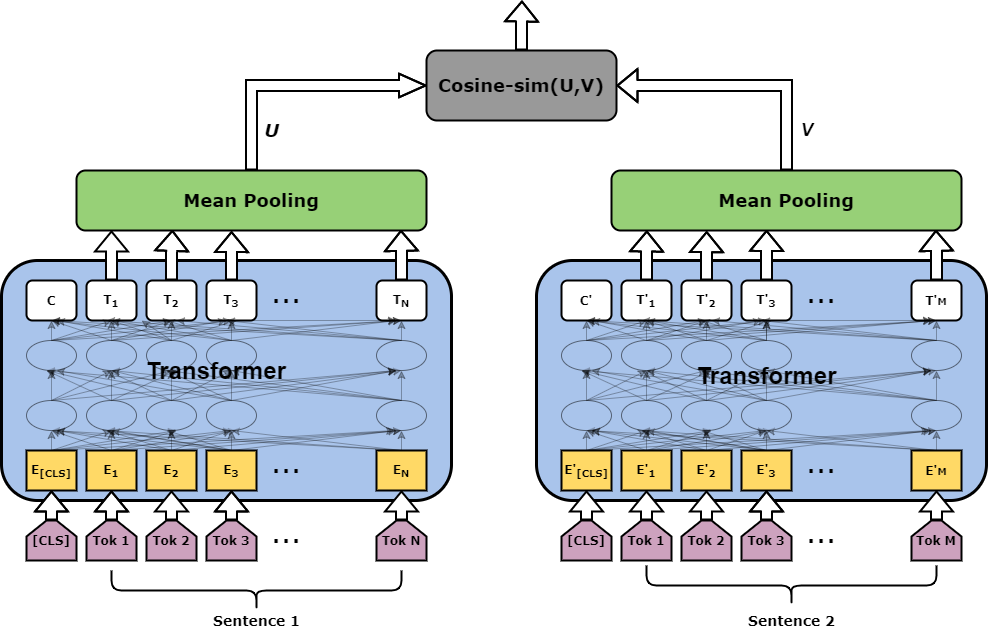
\includegraphics[scale=0.35]{figures/semantic_textual_similarity/transformers/sentence-bert.png}
	\caption[Architecture for using Siamese Transformers in STS]{Architecture for using Siamese Transformers in STS.}
	\label{fig:siamese_transformers}
\end{figure}

As we observed in previous experiments, transformers are state-of-the-art in supervised STS. However, to predict the similarity in test time, both sentences must be fed into the network. Two sentences are passed to the transformer network, and the similarity is predicted. However, this setup is unsuitable for various text similarity tasks. For example, finding the sentence pair with the highest similarity in a collection of n = 10 000 sentences requires $n \times \frac {(n-1)}{2} = 49,995,000$ inference computations with the default transformer architecture experimented in this chapter. On a modern V100 GPU, this requires about 65 hours. Similarly, finding the most similar question for a new question from over 40 million existing questions in Quora would require over 50 hours. This massive computational overload is not suitable for many real-world applications \autocite{reimers-gurevych-2019-sentence}.

The obvious solution to this would be to get sentence embeddings from the transformer network. A common approach is to use vector aggregation methods that we already experimented in Chapter \ref{cha:sts_state_of_the_art_methods}. However, we previously showed that these simple, unsupervised vector aggregation-based STS methods are outperformed by sentence encoders that use traditional word embeddings. Therefore, \textcite{reimers-gurevych-2019-sentence} propose a Siamese neural architecture based on transformers. The architecture is shown in Figure \ref{fig:siamese_transformers}, which is similar to the Siamese architectures we experimented in Chapter \ref{cha:sts_siamese_neural_networks}.

This architecture can be trained on an STS dataset. Since this is a Siamese architecture, it can produce sentence embeddings that can be used at the inference time without having both sentences in the network. \textcite{reimers-gurevych-2019-sentence} show that this architecture provides less accuracy than the default transformer architecture in STS tasks. Yet, the results are very compatible and outperform other sentence encoders such as Universal Sentence Encoder and Infersent. Furthermore, it outperforms the word embedding based Siamese neural network architectures experimented in Chapter \ref{cha:sts_siamese_neural_networks}. Therefore, this architecture is the current state-of-the-art Siamese neural network in STS tasks. \textcite{reimers-gurevych-2019-sentence} calculate that the complexity for finding the most similar sentence pair in a collection of 10,000 sentences is reduced from 65 hours with the default architecture to 5 seconds with the Siamese transformer architecture. We can conclude that this architecture is very efficient in many NLP applications where it is required to find similar sentences from a large set of sentences, such as Translation Memories\footnote{More details and the pre-trained models on Siamese transformers are available on \url{https://www.sbert.net/}}.  


\section{Conclusions}
In this chapter, we experimented with utilising state-of-the-art transformers in the STS task. We evaluated the default sentence pair regression architecture on transformers in three English datasets, two non-English datasets and a bio-medical STS dataset. For the smaller STS datasets, we showed that \textit{RoBERTa} outperformed other transformer models. For the larger STS dataset, \textit{XLNET} provided the best result. We showed that we could improve the results with transfer learning and data augmentation techniques. For the three English and two non-English datasets, the transformer-based STS method outperformed all the other supervised and unsupervised STS methods we experimented with in this part of the thesis. Furthermore, they outperformed the best systems submitted for each competition. This shows that the transformers are the current state-of-the-art in supervised STS.

However, in the BIOSSES dataset where it does not have a training set, we used a transfer learning based zero-shot learning when transformers are applied. Even though transformers outperformed other STS methods we experimented such as Siamese neural networks, they could not outperform the sentence vector-based method we experimented with in Chapter \ref{cha:sts_sentence_encoders}. We can conclude that although the transformers can be adapted in different domains by changing the pre-trained model, they do not provide strong results without a proper training set. 

One major limitation in the transformer-based STS method is that it requires to have both sentences in the network at the inference time, which can cause a massive computational overhead for some NLP applications. To overcome this, \textcite{reimers-gurevych-2019-sentence} proposed a Siamese transformer architecture that is capable of proving sentence vectors that can reduce the inference time. Another limitation in the transformers is the pre-trained transformer models are large and can cause problems in real-world applications. As a solution to this, we hope to explore knowledge distillation \autocite{Gou2021} in STS tasks. With knowledge distillation, transformer-based methods can be used as teacher models to train simple student models such as Siamese GRU, which would provide competitive results to transformer-based STS methods but with smaller disk space. 

With this, we conclude Part I of the thesis. We explored numerous STS methods based on word vectors which are easy to adapt in different languages and domains. We evaluated them on different STS datasets and discussed their benefits and limitations in each chapter. We can conclude that transformers are state-of-the-art in supervised STS methods and sentence encoders are state-of-the-art in unsupervised STS methods. Keeping in mind the benefits and limitations of these STS methods, in the following two parts of the thesis, we will employ them in two applications in translation technology; translation memories in Part II and translation quality estimation in Part III.



\part{Applications - Translation Memories}
\chapter{\label{cha:tm_introduction}Introduction}

\section{What is Translation Memory?}
\cite{Arthern1979}
\section{Datasets}

\section{Related Work}

\section{STS for Translation Memories}




\chapter{\label{cha:sentence_encoders}Sentence Encoders for Translation Memories}

\cite{ranasinghe-etal-2020-intelligent}

\section{Methodology}

\section{Results and Evaluation}

\part{Applications - Translation Quality Estimation}
\definecolor{applegreen}{rgb}{0.55, 0.71, 0.0}
\definecolor{brickred}{rgb}{0.8, 0.25, 0.33}
\definecolor{asparagus}{rgb}{0.53, 0.66, 0.42}

\DeclareRobustCommand{\hlgreen}[1]{{\sethlcolor{asparagus}\hl{#1}}}

\DeclareRobustCommand{\hlred}[1]{{\sethlcolor{brickred}\hl{#1}}}

\newcommand{\hlc}[2][yellow]{{%
		\colorlet{foo}{#1}%
		\sethlcolor{foo}\hl{#2}}%
}


\chapter{\label{cha:qe_introduction}Introduction to Translation Quality Estimation}

The goal of quality estimation (QE) is to evaluate the quality of a translation without having access to a reference translation \autocite{specia-etal-2018-findings}. High-accuracy QE that can be easily deployed for a number of language pairs is the missing piece in many commercial translation workflows as they have numerous potential uses. They can be employed to select the best translation when several translation engines are available or can inform the end-user about the reliability of automatically translated content. In addition, QE systems can be used to decide whether a translation can be published as it is in a given context, or whether it requires human post-editing before publishing or even translation from scratch by a human  \autocite{kepler-etal-2019-openkiwi}. 

Quality estimation task is different from automatic machine translation evaluation \autocite{barrault-etal-2020-findings}. Automatic machine translation evaluation approaches such as BLEU \autocite{papineni-etal-2002-bleu} need the reference translation in order to perform the machine translation evaluation. As mentioned before, quality estimation, on the other hand, does not need the reference translation. Therefore, automatic MT evaluation approaches such as BLEU \autocite{papineni-etal-2002-bleu}, METEOR \autocite{banerjee-lavie-2005-meteor}, LEPOR \autocite{han-etal-2012-lepor} and others can not be directly applied in the QE task. As a result, the solutions proposed for QE are completely different from that of automatic machine translation evaluation.

The estimation of translation quality can be done at different levels: word/phrase-level, sentence-level and, document-level \autocite{ive-etal-2018-deepquest}. Word-level QE aims to spot words that need to be reviewed during the post-editing process. It indicates which words from the source have been incorrectly translated in the target and whether the words inserted between these words are correct. Sentence-level QE models provide a single score for each pair of source and target sentences. Sentence-level QE scores help to rank translations that are worth post-editing. Document-level QE, on the other hand, scores or ranks documents according to their quality for fully automated MT usage scenarios \autocite{ive-etal-2018-deepquest}. In recent years, word-level QE and sentence-level QE have been more popular among the community \autocite{specia-etal-2018-findings}.

During the past decade, there has been tremendous progress in the field of quality estimation, largely as a result of the QE shared tasks organised annually by the Workshops on Statistical Machine Translation (WMT), more recently called as the Conferences on Machine Translation, since 2012  \autocite{callison-burch-etal-2012-findings,bojar-etal-2013-findings,bojar-etal-2014-findings,bojar-etal-2015-findings,bojar-etal-2016-findings,bojar-etal-2017-findings,specia-etal-2018-findings,fonseca-etal-2019-findings,specia-etal-2020-findings-wmt}. Firstly, they have provided annotated datasets which can be used to train QE models and to evaluate them. Secondly, the annotated datasets these shared tasks released each year have led to the development of many open-source QE systems \autocite{specia-etal-2015-multi, ive-etal-2018-deepquest, kepler-etal-2019-openkiwi}. 

At present neural-based QE methods constitute state-of-the-art in quality estimation. However, these approaches are based on complex neural networks and require resource-intensive training. This resource-intensive nature of these deep learning based frameworks makes it expensive to train QE models. Furthermore, these architectures require a large number of annotated instances for training, making the quality estimation task very difficult for the low-resource language pairs. This nature of the current state-of-the-art QE systems has hindered their popularity in real-world applications.

This part of the thesis addresses these problems by employing simple STS architectures we experimented with in Part I of the thesis in quality estimation. We redefine the QE task as a cross-lingual STS task and show that state-of-the-art STS architectures can be applied in the QE task by changing the input embeddings. As far as we know, this is the first study done on applying neural STS models directly to the QE task. 

In Chapter \ref{cha:qe_transquest}, we explore sentence-level QE with STS architectures. We evaluate their performance in recent sentence-level QE datasets, comparing them with open-source QE tools such as OpenKiwi \autocite{kepler-etal-2019-openkiwi} and QuEst++ \autocite{specia-etal-2015-multi}. Finally, we propose a new state-of-the-art QE method for sentence-level QE.

In Chapter \ref{cha:qe_word}, we expand this idea to word-level QE. We modify the output of the STS architecture to predict word-level translation qualities. We evaluated their performance in recent word-level QE datasets, comparing the results with open-source word-level QE tools such as OpenKiwi \autocite{kepler-etal-2019-openkiwi} and Marmot \autocite{logacheva-etal-2016-marmot}. We show that in most of the datasets, our simple word-level architecture outperforms other QE tools. 

In Chapter \ref{cha:qe_multilingual}, for the first time, we explore multilingual QE with state-of-the-art word-level and sentence-level QE methods. Furthermore, we evaluate multilingual QE in different training environments, including zero-shot and few-shot. Our findings in Chapter \ref{cha:qe_multilingual} would be beneficial for low resource languages. 


The main contributions of this part of the thesis are as follows.

\begin{enumerate}

	\item We propose two STS architectures based on transformers to perform sentence-level QE. These architectures are simpler than the  architectures available in OpenKiwi \autocite{kepler-etal-2019-openkiwi} and DeepQuest \autocite{ive-etal-2018-deepquest}. We evaluate them on 15 language pairs in which sentence-level QE data was available, and we show that the two architectures outperform the current state-of-the-art sentence-level QE frameworks such as OpenKiwi \autocite{kepler-etal-2019-openkiwi} and DeepQuest \autocite{ive-etal-2018-deepquest}.
	
	
	\item We introduce a simple architecture to perform word-level quality estimation that predicts the quality of the words in the source sentence, target sentence and the gaps in the target sentence. We evaluate it on eight different language pairs in which the word-level QE data was available, and we show that the proposed architecture outperforms the current state-of-the-art word-level QE frameworks like Marmot \autocite{logacheva-etal-2016-marmot} and OpenKiwi \autocite{kepler-etal-2019-openkiwi}.

	\item We propose multilingual learning for QE with the proposed architectures for sentence-level and word-level. We show that multilingual models are helpful in low-resource languages where the training data is difficult to find. 
	
	\item We provide important resources to the community. The code of each chapter is bundled to an open-source QE framework, and the pre-trained sentence-level and word-level QE models will be freely available to the community. The link to the relevant code and the models will be unveiled in the introduction section of each chapter. 
\end{enumerate}

The remainder of this chapter is structured as follows. Section \ref{sec:qe_related} explores the various methods that have been employed in sentence-level and word-level QE, including previous research done incorporating STS in the QE task. Section \ref{sec:qe_datasets} discuss the various datasets we used in this part of the thesis. In Section \ref{sec:qe_evaluation}, we show the main evaluation metrics used for the sentence-level and word-level QE experiments in the following Chapters in Part III of the thesis. The chapter finishes with the conclusions.



\section{Related Work}
\label{sec:qe_related}
Before the neural network era, most of the quality estimation systems such as QuEst \autocite{specia-etal-2013-quest} and QuEst++ \autocite{specia-etal-2015-multi} were heavily dependent on linguistic processing and feature engineering to train traditional machine-learning algorithms including support vector regression and randomised decision trees \autocite{specia-etal-2013-quest}. These features can be either extracted from the machine translation system (\textit{glass-box} features) or obtained from
the source and translated sentences, as well as external resources, such as monolingual or parallel corpora (\textit{black-box} features) \autocite{specia-etal-2009-estimating}. For example, QuEst \autocite{specia-etal-2013-quest} has 17 manually crafted features fed into a support vector regression algorithm. These 17 features consist of glass-box features such as \textit{ratio of number of tokens in source and target segments}, \textit{ratio of percentage of nouns/verbs in the source and target} etc. as well as black-box features such as \textit{global score and relevant features of the SMT system}, \textit{proportion of pruned search graph nodes} etc. In QuEst++, the number of features varies from 80 to 123 depending on the language pair \autocite{specia-etal-2015-multi}. QuEst \autocite{specia-etal-2013-quest}, QuEst++ \autocite{specia-etal-2015-multi} and Marmot \autocite{logacheva-etal-2016-marmot} can be considered as the most popular traditional QE tools. QuEst \autocite{specia-etal-2013-quest} only supports sentence-level QE, Marmot \autocite{logacheva-etal-2016-marmot} only supports word-level QE while QuEst++ \autocite{specia-etal-2015-multi} can support both word-level and sentence-level QE. Even though, they provided good results in early days, these traditional approaches are no longer the state-of-the-art. In recent years, neural-based QE systems have consistently topped the leader boards in WMT quality estimation shared tasks  \autocite{kepler-etal-2019-openkiwi}.  

With the increasing popularity of word embeddings \autocite{DBLP:journals/corr/abs-1301-3781}, neural networks based on word embeddings got popular in the QE field. They outperformed traditional QE systems and provided state-of-the-art results. For example, the best-performing system at the WMT 2017 shared task on QE was \textsc{POSTECH}, which is purely neural and does not rely on feature engineering at all \autocite{kim-etal-2017-predictor}. \textsc{POSTECH} revolves around an encoder-decoder Recurrent Neural Network (RNN) (referred to as the `predictor'), stacked with a bidirectional RNN (the `estimator') that produces quality estimates. In the predictor, an encoder-decoder RNN model predicts words based on their context representations and in the estimator step, there is a bidirectional RNN model to produce quality estimates for words, phrases and sentences based on representations from the predictor. To be effective, \textsc{POSTECH} requires extensive predictor pre-training, which means it depends on large parallel data and is computationally intensive \autocite{ive-etal-2018-deepquest}. The \textsc{POSTECH} architecture was later re-implemented in DeepQuest  \autocite{ive-etal-2018-deepquest}. DeepQuest supports both word-level and sentence-level QE \autocite{ive-etal-2018-deepquest}. 

OpenKiwi \autocite{kepler-etal-2019-openkiwi} is another open-source neural QE framework developed by Unbabel. It implements four different neural network architectures \textsc{QUETCH} \autocite{kreutzer-etal-2015-quality}, \textsc{NuQE} \autocite{martins-etal-2016-unbabels}, Predictor-Estimator \autocite{kim-etal-2017-predictor} and a stacked model of these architectures. Both the \textsc{QUETCH} and \textsc{NuQE} architectures have simple neural network models that do not rely on additional parallel data but do not perform that well. The Predictor-Estimator model is similar to the \textsc{POSTECH} architecture and relies on additional parallel data. In OpenKiwi, the best performance for sentence-level quality estimation was given by the stacked model that used the Predictor-Estimator model, meaning that the best model requires extensive predictor pre-training and relies on large parallel data and computational resources. 

As discussed before, these models' complex and resource-intensive nature creates many limitations when deployed in real-world scenarios. Therefore, in this study, we propose to use simple STS architectures in QE. Over the years, there have been a few attempts to integrate semantic similarity into QE. \textcite{specia2011predicting} employed semantic information into the QE task to address the problem of meaning preservation in translation. The authors integrated semantic similarity features to the QE model and improved the results of the QE task \autocite{specia2011predicting}. \textcite{bicici-way-2014-referential} introduced the use of referential translation machines (RTM) for QE. RTM is a computational model for judging monolingual and bilingual similarity that achieves state-of-the-art results. This approach provided the best result in both sentence-level and word-level tasks in WMT 2013 \autocite{bojar-etal-2013-findings}. Furthermore, \textcite{kaljahi-etal-2014-syntax} and \textcite{camargo-de-souza-etal-2014-fbk} used syntactic and semantic information in quality estimation and were able to improve over the baseline when combining these features with the features of the baseline. Finally, in a different approach, \textcite{bechara-etal-2016-semantic} used semantically similar sentences and their quality scores as features to estimate the quality of machine translated sentences. This method improved the prediction of machine translation quality for semantically similar sentences \autocite{bechara-etal-2016-semantic}. 

Even though there are several studies done to integrate semantic similarity into QE, as far as we know, this is the first study to employ state-of-the-art neural STS models directly in the QE task. 

\section{Datasets}
\label{sec:qe_datasets}

 All the datasets that we used in this part of the thesis are publicly available and were released in WMT quality estimation tasks in recent years \autocite{specia-etal-2018-findings,fonseca-etal-2019-findings,specia-etal-2020-findings-wmt}. This was done to ensure the replicability of our experiments and to allow us to compare our results with state-of-the-art methods. The following sections will describe the sentence-level and word-level QE datasets we experimented, separately.

\subsection{Sentence-level QE}
Sentence-level QE datasets that we used in this part of the thesis can be categorised into two main areas depending on the aspect they have been annotated; Human-mediated Translation Edit Rate (HTER) and Direct Assessment (DA). Most of the early datasets have been annotated on HTER. Very recently DA aspect is getting popular in the QE community. We describe each of them in detail in the following sections.


\paragraph{Predicting HTER}
The performance of sentence-level QE systems has typically been assessed using the semiautomatic HTER. HTER is an edit-distance-based measure that captures the distance between the automatic translation and a reference translation in terms of the number of modifications required to transform one into another. In light of this, a QE system should be able to predict the percentage of edits required in the translation. We used several language pairs for which HTER information was available: English-Chinese (En-Zh), English-Czech (En-Cs), English-German (En-De), English-Russian (En-Ru), English-Latvian (En-Lv) and German-English (De-En). The texts are from a variety of domains, and the translations were produced using both neural and statistical machine translation systems. More details about these datasets can be found in Table \ref{tab:hter_data} and in \autocite{specia-etal-2018-findings,fonseca-etal-2019-findings,specia-etal-2020-findings-wmt}. Several examples from WMT 2020, En-De dataset is shown in Table \ref{tab:hter_data_examples}.

\begin{table}[t]
	\begin{center}
		\scalebox{0.65}{
		\begin{tabular}{ |c|c|c|c|c| } 
			\hline
			\textbf{Language Pair} & \textbf{Source} & \textbf{MT system} & \textbf{Competition} &  \textbf{train, dev, test size} \\ 
			\hline
			De-En & Pharmaceutical & Phrase-based SMT & WMT 2018 \autocite{specia-etal-2018-findings} & 25,963, 1,000, 1,000  \\
			\hline
			En-Zh & Wiki & fairseq based NMT & WMT 2020 \autocite{specia-etal-2020-findings-wmt} & 7,000, 1,000, 1,000 \\
			\hline
			En-Cs & IT & Phrase-based SMT & WMT 2018 \autocite{specia-etal-2018-findings} & 40,254, 1,000, 1,000 \\
			\hline
			En-De & Wiki & fairseq based NMT & WMT 2020 \autocite{specia-etal-2020-findings-wmt} & 7,000, 1,000, 1,000 \\
			\hline
			En-De & IT & Phrase-based SMT & WMT 2018 \autocite{specia-etal-2018-findings}  & 26,273, 1,000, 1,000 \\
			\hline
			En-Ru & Tech & Online NMT & WMT 2019 \autocite{fonseca-etal-2019-findings} & 15,089, 1,000, 1,000 \\
			\hline
			En-Lv & Pharmaceutical & Attention-based NMT & WMT 2018 \autocite{specia-etal-2018-findings} & 12,936, 1,000, 1,000 \\
			\hline
			En-Lv & Pharmaceutical & Phrase-based SMT & WMT 2018 \autocite{specia-etal-2018-findings}  & 11,251, 1,000, 1,000 \\
			\hline
		\end{tabular}
	}
	\end{center}
	\caption[Information about language pairs used to predict HTER]{Information about language pairs used to predict HTER. The \textbf{Language Pair} column shows the language pairs we used in ISO 639-1 codes\protect\footnotemark. \textbf{Source} expresses the domain of the sentence and \textbf{MT system} is the Machine Translation system used to translate the sentences. 
		In that column NMT indicates Neural Machine Translation and SMT indicates Statistical Machine Translation. 
		\textbf{Competition} shows the quality estimation competition in which the data was released and the last column indicates the number of instances the train, development and test dataset had in each language pair respectively.} 
	\label{tab:hter_data}
\end{table}

\footnotetext{Language codes are available in ISO 639-1 Registration Authority Website Online - \url{ https://www.loc.gov/standards/iso639-2/php/code_list.php}}

\begin{table}[t] 
	\centering
	\scalebox{0.95}{
		\begin{tabular}{ |p{5.5cm}|p{5.5cm}|c| }
			\hline
			\multicolumn{1}{|c|}{\textbf{Source}}  & \multicolumn{1}{c|}{\textbf{Target}}  & \textbf{HTER}  \\
			\hline
			José Ortega y Gasset visited Husserl at Freiburg in 1934 . & 1934 besuchte José Ortega y Gasset Husserl in Freiburg . & 0.3333 \\
			\hline
			however , a disappointing ninth in China meant that he dropped back to sixth in the standings . & eine enttäuschende Neunte in China bedeutete jedoch , dass er in der Gesamtwertung auf den sechsten Platz zurückfiel . & 0.2000 \\
			\hline
			" Renaissance Humanism and the Future of the Humanities . " & " Renaissance Humanism and the Future of the Humanities " . & 1.0000 \\
			\hline
		sophomore Jacory Harris directed the newly implemented offense . & Sophomore Jacory Harris leitete die neu umgesetzte Straftat . & 0.0000 \\
			\hline
			
		\end{tabular}
	}
	\caption[Examples source/target pairs from WMT 2020 En-De HTER dataset.]{Examples source/target pairs from WMT 2020 En-De HTER dataset \autocite{specia-etal-2020-findings-wmt}.  \textbf{Source} column shows the source sentence in English and \textbf{Target} shows the target sentence in German. \textbf{HTER} column shows the annotated HTER value for the translation. 
	}
	\label{tab:hter_data_examples}
\end{table}



\paragraph{Predicting DA}
Even though HTER has been typically used to assess quality in machine translations, the reliability of this metric for evaluating the performance of quality estimation systems has been questioned by researchers \autocite{graham-etal-2016-glitters}. The current practice in MT evaluation is the so-called Direct Assessment (DA) of MT quality \autocite{graham_baldwin_moffat_zobel_2017}, where raters evaluate the machine translation on a continuous 1-100 scale. This method has been shown to improve the reproducibility of manual evaluation and to provide a more reliable gold standard for automatic evaluation metrics \autocite{graham-etal-2015-accurate}. 

We used a recently created dataset to predict DA in machine translations which was released for the WMT 2020 quality estimation shared task 1 \autocite{specia-etal-2020-findings-wmt}. The dataset is composed of data extracted from Wikipedia for six language pairs, consisting of high-resource English-German (En-De) and English-Chinese (En-Zh), medium-resource Romanian-English (Ro-En) and Estonian-English (Et-En), and low-resource Sinhala-English (Si-En) and Nepalese-English (Ne-En), as well as a Russian-English (En-Ru) dataset which combines articles from Wikipedia and Reddit \autocite{fomicheva-etal-2020-unsupervised}. These datasets have been collected by translating sentences sampled from source-language articles using state-of-the-art NMT models built using the fairseq toolkit \autocite{ott-etal-2019-fairseq} and annotated with DA scores by professional translators. Each translation was rated with a score from 0-100 according to the perceived translation quality by at least three translators \autocite{specia-etal-2020-findings-wmt}. The DA scores were standardised using the z-score. The quality estimation systems evaluated on these datasets have to predict the mean DA z-scores of test sentence pairs. Each language pair has 7,000 sentence pairs in the training set, 1,000 sentence pairs in the development set and another 1,000 sentence pairs in the testing set. 

 \begin{table}[t] 
 	\centering
 	\scalebox{0.95}{
 		\begin{tabular}{ |p{5.5cm}|p{5.5cm}|c| }
 			\hline
 			\multicolumn{1}{|c|}{\textbf{Source}}  & \multicolumn{1}{c|}{\textbf{Target}}  & \textbf{DA}  \\
 			\hline
 		Tratatul de Aderare fusese semnat la 16 aprilie 2003. & The Accession Treaty had been signed on 16 April 2003. & 0.6226 \\
 			\hline
 			Are o industrie turistică bine dezvoltată, fiind o destinație populară printre turiștii britanici și germani. & It has a well-developed tourist industry as a popular destination among British and German tourists. & 0.9386 \\
 			\hline
 			Numărul mare de avioane de vânătoare trimise în misiuni împotriva avioanelor de recunoaștere nu a fost o greșeală. & There was no mistake in the large number of hunting aeroplanes deployed in missions against recognition aeroplanes.	 & 0.0024 \\
 			\hline
 			Ar fi fost inutil să încerce obținerea unei o catedre universitare. & It would have been pointless to try to get a university catalogue. & 0.5456 \\
 			\hline
 			
 		\end{tabular}
 	}
 \caption[Examples source/target pairs from WMT 2020 Ro-En DA dataset.]{Examples source/target pairs from WMT 2020 Ro-En DA dataset \autocite{specia-etal-2020-findings-wmt}.  \textbf{Source} column shows the source sentence in English and \textbf{Target} shows the target sentence in German. \textbf{DA} column shows the annotated DA value for the translation. 
 }
 	\label{tab:da_data_examples}
 \end{table}

\subsection{Word-level QE}
Word-level QE annotations are not straightforward as sentence-level QE annotations. They have been annotated for words in the target (`OK' for correct words, `BAD' for incorrect words), gaps in the target (`OK' for genuine gaps, `BAD' for gaps indicating missing words) and source words (`BAD' for words that lead to errors in the target, `OK' for other words) \autocite{specia-etal-2018-findings}. To make it clearer, consider the following example from En-De in WMT 2018 \autocite{specia-etal-2018-findings}. The word-level quality estimation labels would be followed. Please note that \textit{green} represents `OK' and \textit{red} represents `BAD' labels. 


\noindent \textbf{Source} - \textit{for example , you could create a document containing a car that moves across the Stage .}

\noindent \textbf{Target} - \textit{Sie können beispielsweise ein Dokument erstellen , das ein Auto über die Bühne enthält .}


\noindent \textbf{Source} - \textit{\hlgreen{for} \hlgreen{example} \hlgreen{,} \hlgreen{you} \hlgreen{could} \hlgreen{create} \hlgreen{a} \hlgreen{document} \hlgreen{containing} \hlred{a} \hlred{car} \hlred{that} \hlred{moves} \hlgreen{across} \hlgreen{the} \hlgreen{Stage} \hlgreen{.}}



\noindent \textbf{Target} - \textit{\hlgreen{<GAP>} \hlgreen{Sie} \hlgreen{<GAP>} \hlgreen{können} \hlgreen{<GAP>} \hlgreen{beispielsweise} \hlgreen{<GAP>} \hlgreen{ein} \hlgreen{<GAP>} \hlgreen{Dokument} \hlgreen{<GAP>} \hlgreen{erstellen} \hlgreen{<GAP>} \hlgreen{,} \hlgreen{<GAP>} \hlgreen{das} \hlgreen{<GAP>} \hlgreen{ein} \hlgreen{<GAP>} \hlgreen{Auto} \hlred{<GAP>} \hlgreen{über} \hlgreen{<GAP>} \hlgreen{die} \hlgreen{<GAP>} \hlgreen{Bühne} \hlgreen{<GAP>} \hlred{enthält} \hlgreen{<GAP>} \hlgreen{.} \hlgreen{<GAP>}}


As can be seen in the example, all the words in the source, all the words in the target and all the \textit{gaps} in the target have been annotated as `OK' or `BAD'.  Most of the language pairs that are annotated for sentence-level HTER scores also have word-level quality labels. Therefore, for the word-level QE experiments, we used the same language pairs we used for sentence-level HTER, which are shown in Table \ref{tab:hter_data}. More information about the word-level annotations are available on \autocite{specia-etal-2018-findings,fonseca-etal-2019-findings,specia-etal-2020-findings-wmt}.


\section{Evaluation}
\label{sec:qe_evaluation}
For the evaluation, we used the same approach proposed in the WMT shared tasks so that we can compare our results with the respective baselines and the best systems submitted in each shared task. Obviously, the sentence-level and word-level QE follow two different evaluation criteria, which we explain in the following sections. 

\paragraph{Sentence-Level QE Evaluation} : Similar to the STS evaluation in Part I of the thesis, Pearson's Correlation Coefficient ($\rho$) is the most popular evaluation metric in recent WMT sentence-level QE shared tasks \autocite{specia-etal-2018-findings,fonseca-etal-2019-findings,specia-etal-2020-findings-wmt}. Since the gold labels are continuous in both HTER and DA and the models need to predict a continuous value, it makes sense to employ Pearson's Correlation Coefficient as the evaluation metric. A QE model with a Pearson's Correlation Coefficient close to 1 indicates that the predictions of that model and gold labels have a strong positive linear correlation, and therefore, it is a good model to predict sentence-level QE.  


\paragraph{Word-level QE Evaluation} : The primary evaluation metric for word-level QE is the multiplication of F1-scores for the OK and BAD classes, denoted as $F1_{\textit{MULTI}}$ \autocite{specia-etal-2018-findings,fonseca-etal-2019-findings,specia-etal-2020-findings-wmt}. The standard equation for the F1 score is shown in Equation \ref{equ:f1} where TP, TN, FP and FN are True Positive, True Negative, False Positive and False Negative, respectively. This F1 score is calculated for OK and BAD classes separately, and then, they are multiplied to get the $F1_{\textit{MULTI}}$ as shown in Equation \ref{equ:f1_multi}. 

\begin{equation}
\label{equ:f1}
	F1 = \frac{2*TP}{2*TP+FP+FN}
\end{equation}


\begin{equation}
	\label{equ:f1_multi}
	F1_{\textit{MULTI}} = F1_{\textit{OK}} \times F1_{\textit{BAD}}
\end{equation}

Prior to WMT 2019, $F1_{\textit{MULTI}}$ score was calculated separately for words in the source ($F1_{\textit{MULTI}} \; Source$), words in the target ($F1_{\textit{MULTI}} \; Target$) and gaps in the target ($F1_{\textit{MULTI}} \; GAPS$) \autocite{specia-etal-2018-findings}, while after WMT 2019 \autocite{fonseca-etal-2019-findings,specia-etal-2020-findings-wmt} they produce a single result for target gaps and words named as "$F1_{\textit{MULTI}} \; Target$" alongside with "$F1_{\textit{MULTI}} \; Source$". We follow the same approach.  A QE model with a $F1_{\textit{MULTI}}$ score close to 1 indicates that the predictions of that model and gold labels are similar and therefore, it is a good model to predict word-level QE.    

\section{Conclusion}
\label{sec:qe_conclusion}
Quality estimation is an important component in making machine translation useful in real-world applications. It aims to inform the user of the quality of the MT output at test time. This process can be done on different levels such as word-level, sentence-level and document-level. QE shared tasks organised annually by WMT have increased QE's popularity among the MT community by leading the development of standard datasets covering a variety of languages and domains. These QE shared tasks have further contributed to the development of evaluation measures in QE.  We followed the same evaluation measures; Pearson's Correlation Coefficient for sentence-level and $F1_{\textit{MULTI}}$ for word-level.

The annotated datasets these shared tasks released each year have led to the development of many open-source QE systems. Similar to other NLP fields, most of the early QE approaches including QuEst \autocite{specia-etal-2013-quest}, QuEst++ \autocite{specia-etal-2015-multi} and Marmot \autocite{logacheva-etal-2016-marmot} were also based on traditional machine learning and involved heavy feature engineering. However, they no longer provide competitive results. The current state-of-the-art in QE is neural models. Following this, many open-source neural QE frameworks such as OpenKiwi \autocite{kepler-etal-2019-openkiwi} and DeepQuest \autocite{ive-etal-2018-deepquest} have been created. However, these neural QE architectures are complex and need a lot of computing resources to train a QE model, which we have identified as a major limitation. To address this weakness, we propose to redefine the QE task as a cross-lingual STS task and apply the STS architectures we experimented in Part I of the thesis to QE, which are considerably simpler than the current state-of-the-art QE models.

In the next few chapters, we will be exploring the STS architectures in the QE task. First, in Chapter \ref{cha:qe_transquest}, the STS architectures will be applied in sentence-level QE, and then in Chapter \ref{cha:qe_word}, these architectures will be extended to word-level QE. Finally, in Chapter \ref{cha:qe_multilingual}, we explore multilingual QE with the proposed architectures.

\chapter{\label{cha:transquest}TransQuest: STS Architectures for QE}

\section{Introduction}
\cite{conneau-etal-2020-unsupervised} 
\section{Methodology}


\begin{figure}
	\centering
	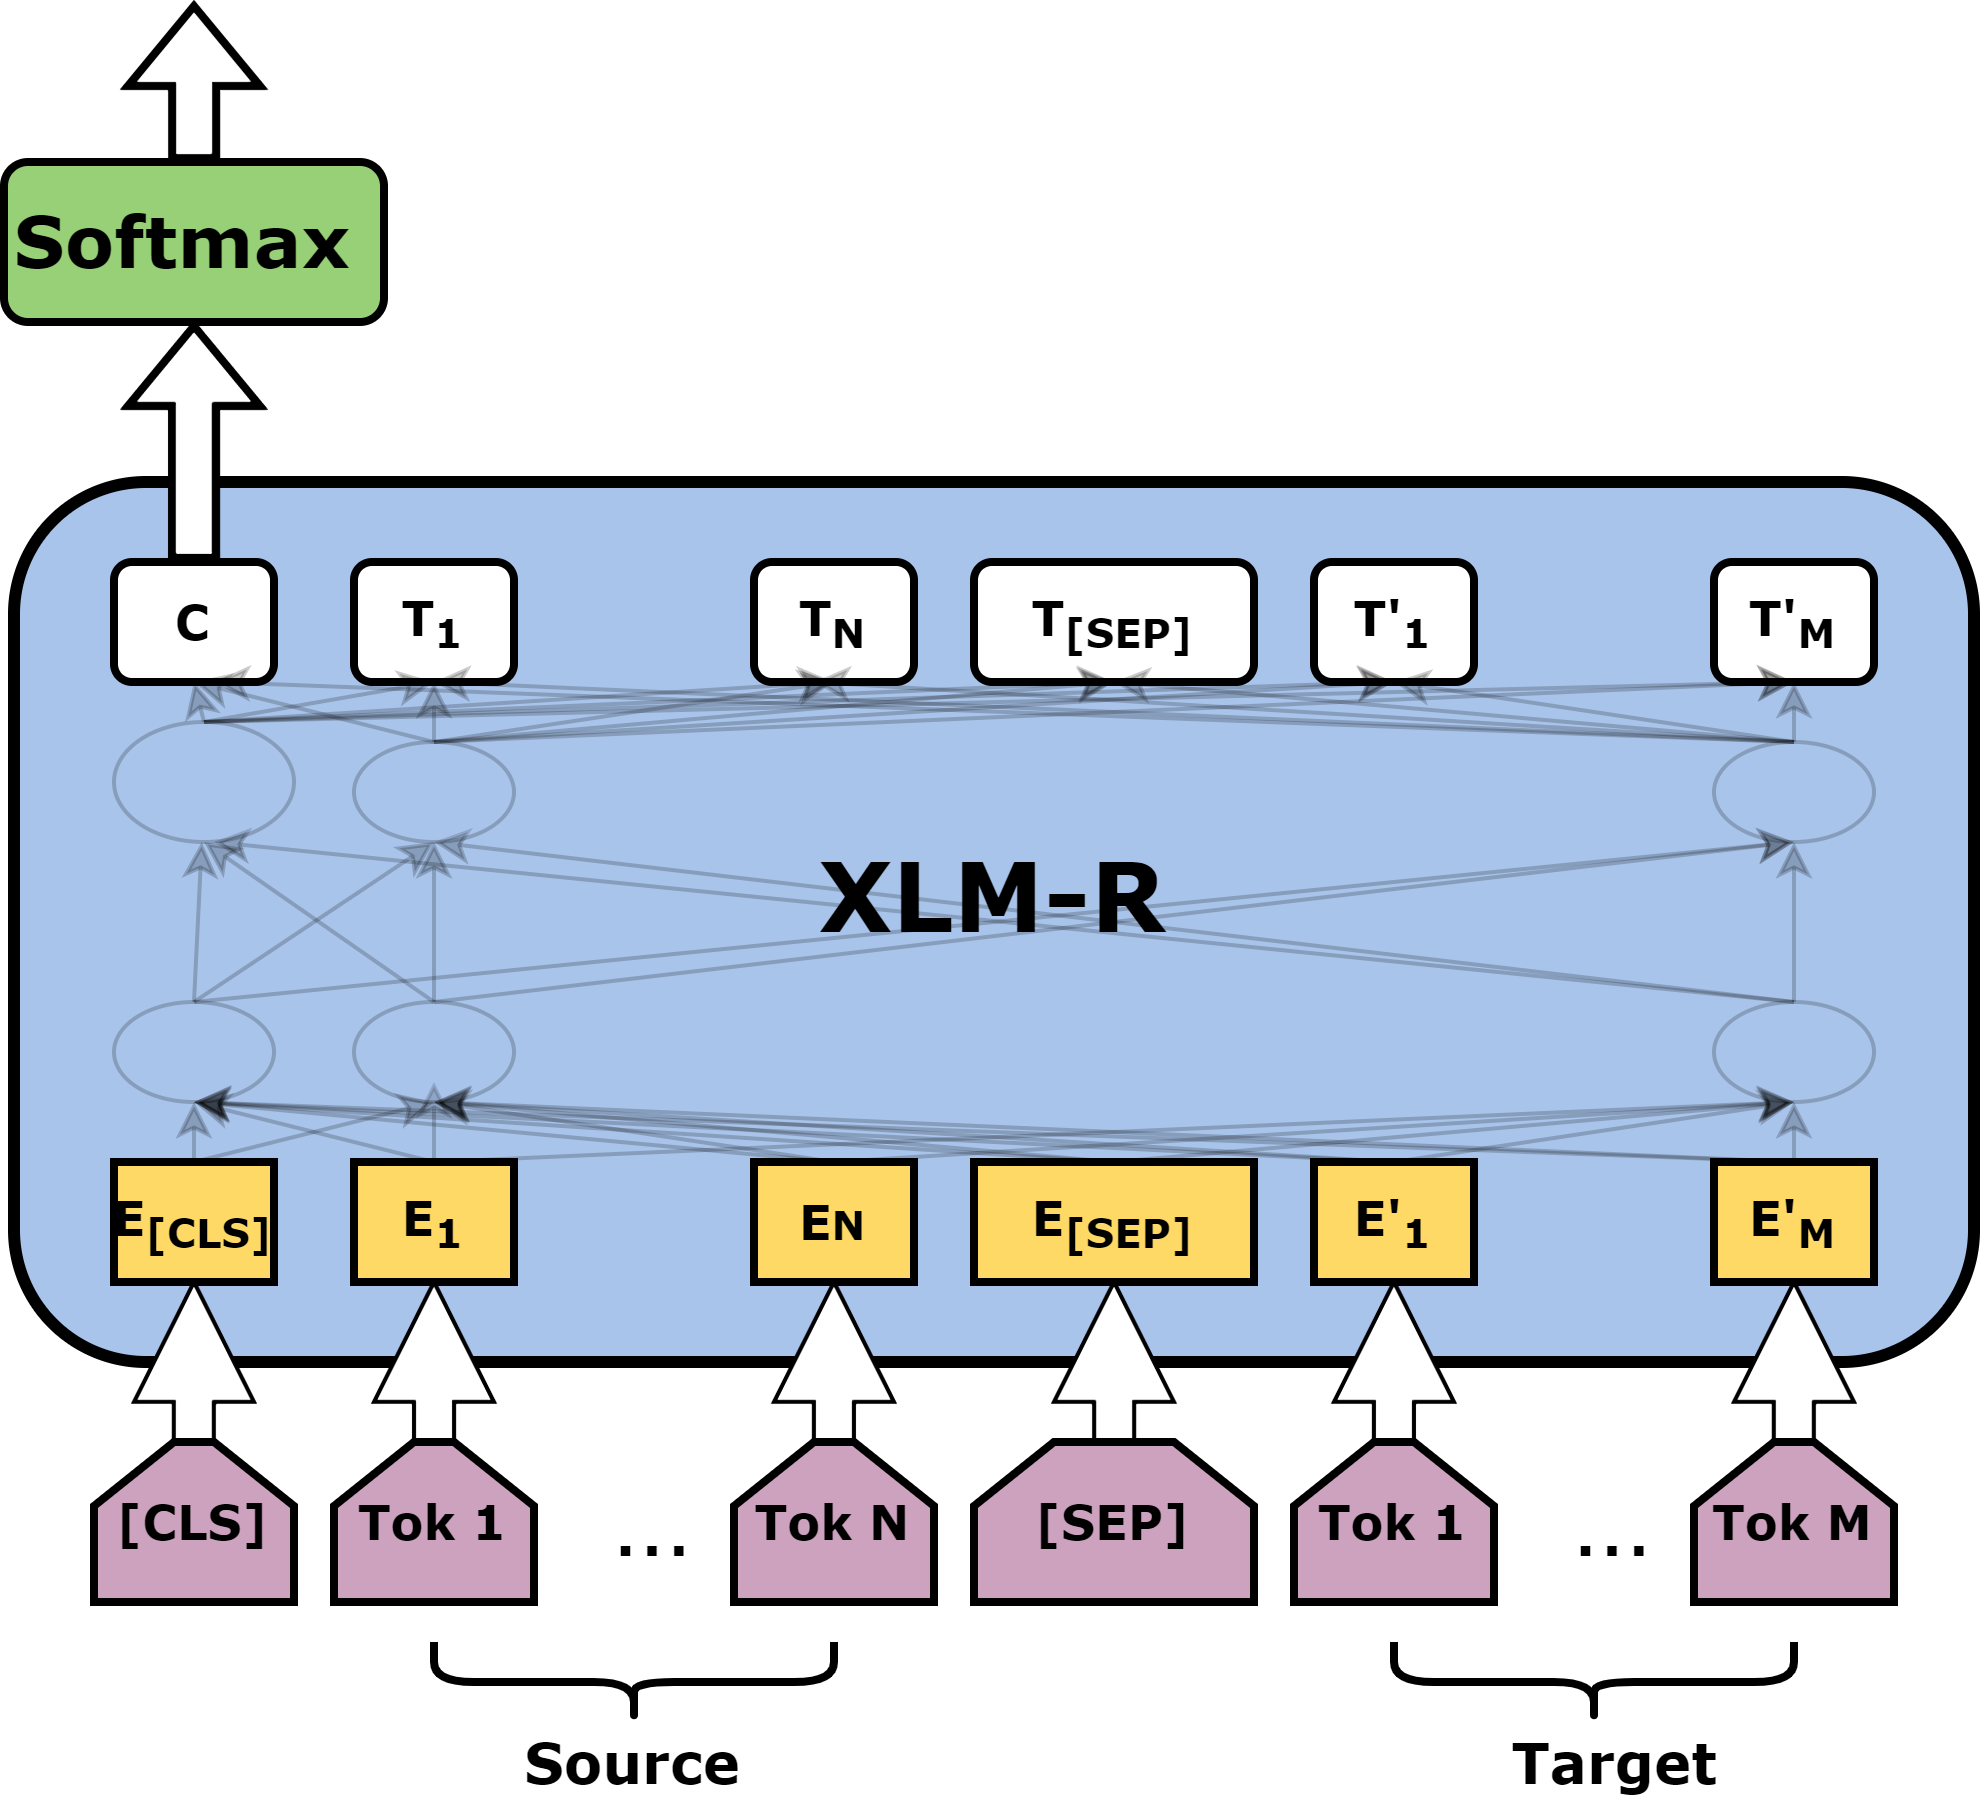
\includegraphics[scale=0.60]{figures/translation_quality_estimation/TransQuest.png}
	\caption{\textit{MonoTransQuest} architecture}
	\label{fig:transquest_architecture}
\end{figure}


\section{Results and Evaluation}


\renewcommand{\arraystretch}{1.2}
\begin{table}[t]
	\begin{center}
		\small
		% \footnotesize
		\scalebox{0.8}{
		\begin{tabular}{l l  c c c c c c c c} 
			%\hline
			\toprule
			& & \multicolumn{4}{c}{\bf Mid-resource} & \multicolumn{4}{c}{\bf High-resource}\\\cmidrule(r){3-6}\cmidrule(r){7-10}
			&{\bf Method} & \makecell{En-Cs \\ SMT} & \makecell{ En-Ru \\ NMT} & \makecell{En-Lv \\ SMT} & \makecell{En-Lv \\ NMT} & \makecell{De-En \\ SMT} & \makecell{En-Zh \\ NMT} & \makecell{En-De \\ SMT } & \makecell{En-De \\ NMT} \\
			\midrule
			\multirow{2}{*}{\bf I} & MTransQuest & \textbf{0.7207} & \textbf{0.7126} & 0.6592 & 0.7394 & \textbf{0.7939} & 0.6119 & 0.7137 & \textbf{0.5994}\\
			& STransQuest & 0.6853 & 0.6723 & 0.6320 & 0.7183 & 0.7524 & 0.5821& 0.6992 & 0.5875 \\
			\midrule
			\multirow{2}{*}{\bf II} & MTransQuest *-En$|$En-* & 0.7168 & 0.7046  & \textbf{0.7181} & \textbf{0.7482} & 0.7939 & 0.6101 & 0.7355 & 0.5992 \\
			& STransQuest *-En$|$En-* & 0.6663 & 0.6701 & 0.6533 & 0.7192 & 0.7524 & 0.5721 & 0.7000 & 0.5793 \\
			\midrule
			\multirow{2}{*}{\bf III} & MTransQuest-m & 0.7111 & 0.7012 & 0.7141 & 0.7450 & 0.7878 & 0.6092 & 0.7300 & 0.5982 \\
			& STransQuest-m & 0.6561 & 0.6614 & 0.6621 & 0.7202 & 0.7369 & 0.5612 & 0.7015 & 0.5771 \\
			%\midrule
			\midrule
			\multirow{3}{*}{\bf IV} & Quest ++ & 0.3943 & 0.2601 & 0.3528 & 0.4435 & 0.3323 & NR & 0.3653 & NR \\
			& OpenKiwi & NR & 0.5923 & NR & NR & NR & 0.5058 & 0.7108 & 0.4001 \\
			& Best system & 0.6918 & 0.5923 & 0.6188 & 0.6819 & 0.7888 & \textbf{0.6641} & \textbf{0.7397} &  0.5718 \\
			\midrule
			\multirow{1}{*}{\bf V} & mBERT & 0.6423 & 0.6354 & 0.5772 & 0.6531 & 0.7005 & 0.5483 & 0.6239 & 0.5002 \\
			\bottomrule
			%\bottomrule
		\end{tabular}
	}
	\end{center}
	\caption[Pearson correlation between TransQuest algorithm predictions and human post-editing effort]{Pearson ($r$) correlation between \textit{TransQuest} algorithm predictions and human post-editing effort. Best results for each language by any method are marked in bold. Rows I, II and III indicate the different evaluation settings. Row IV shows the results of the state-of-the-art methods and the best system submitted for the language pair in that competition. \textbf{NR} implies that a particular result 
		% from a state-of-the-art method 
		was \textit{not reported} by the organisers. Row V presents the results of the multilingual BERT (mBERT) model in MonoTransQuest Architecture.} 
	\label{tab:hter_prediction}
\end{table}
\section{Conclusion}
\chapter{\label{cha:qe_word}Extending TransQuest for Word-Level QE}

Translation quality can be estimated at different levels of granularity: word, sentence and document level \cite{ive-etal-2018-deepquest}. So far in this thesis, we have only explored sentence-level QE \cite{specia-etal-2020-findings-wmt}, in which QE models provide a score for each pair of source and target sentences. A more challenging task, which is currently receiving a lot of attention from the research community, is word-level quality estimation which provides more fine-grained information about the quality of a translation, indicating which words from the source have been incorrectly translated in the target (good vs bad words), and whether the words inserted between these words are correct (good vs bad gaps). This information can be useful for post-editors by indicating the parts of a translation on which they have to focus more. Therefore, word-level QE solutions would certainly improve the efficiency of the post-editors.

Furthermore, as we mentioned before, sentence-level QE models are difficult to explain as they just outputs a single score for the translation. Users would face the difficulty of interpreting the score and deciding the steps after the QE process. However, in contrast to that word-level QE models provide more fine-grained information about the quality of a translation and as a result, they can improve the explainability of the whole QE process. Since there is a growing interest in the NLP community for the explainable machine learning, we believe that having explainable QE models would improve the popularity of QE.   

With these advantages researches have provided many solutions for word-level QE. Similar to sentence-level QE, state-of-the-art models in word-level QE are also relying on deep learning. As we explained in Chapter \ref{cha:qe_introduction}, most of the open source quality estimation frameworks like OpenKiwi, uses same architectures for both word-level and sentence-level QE. For example the predictor-estimator architecture used in OpenKiwi provides best results for word-level QE too. Therefore word-level QE also suffers from the same limitation that we mentioned in last chapter. The architectures are very complex and need a lot of computing resources to train the models which has seriously hindered the success of word-level QE in real-world applications.

To overcome this, we propose a simple architecture to perform word-level QE. The proposed architecture is very similar to the \textit{MonoTransQuest} architecture we introduced in last Chapter which in turn was based on a state-of-the-art STS method. We only change the output layer of the \textit{MonoTransQuest} architecture so that it can retain word-level qualities. This architecture is very simple and effective when compared with the current state-of-the-art word-level QE architectures like predictor-estimator. We believe that a simpler architecture like that would improve the popularity of word-level QE in real-world applications. 

As we mentioned in Chapter \ref{cha:qe_introduction} in Part III of this thesis, word-level QE systems should have three features in them. \textit{i}. Predict the qualities of the words in the target. \textit{ii}. Predict the qualities of the words in the source. \textit{iii}. Predict the qualities of the gaps in the target. As a result, WMT word-level QE shared task has three separate evaluation metrics focussing on each of the above features. However, most of the open source word-level QE frameworks ignore predicting quality of the gaps in the target sentence. For example Marmot \cite{logacheva-etal-2016-marmot} only supports predicting the quality of the words in target and OpenKiwi \cite{kepler-etal-2019-openkiwi} only supports predicting the quality of the words in source and target. They completely ignore predicting the quality of the gaps. Despite that, predicting the quality of the gaps in target would be important and useful for post-editors. Therefore, when we design the proposed architecture in this Chapter, we considered all three features in word-level QE; predicting quality of the words in target, predicting quality of the words in source and predicting quality of the gaps in target. We believe an approach that supports every feature in word-level QE would be stronger than existing solutions.

We address three research questions in this chapter:

\textbf{RQ1:} Can existing state-of-the-art STS architecture be used to predict all features in word-level QE task by just modifying the embeddings and output layer?

\textbf{RQ2:} Does crosslingual embeddings have an advantage over multilingual embeddings in the word-level QE task too?

\textbf{RQ3:} Can the proposed model further improved by performing ensemble learning?

The main contributions of this chapter are as follows.
\begin{enumerate}
  \item We introduce a simple architecture to perform word-level quality estimation that predicts the quality of the words in the source sentence, target sentence and the gaps in the target sentence.
  
  \item We evaluate it on eight different language pairs which the word-level QE data was available and we show that the proposed architecture outperforms the current state-of-the-art word-level QE frameworks like Marmot \cite{logacheva-etal-2016-marmot} and OpenKiwi \cite{kepler-etal-2019-openkiwi}.
  
  \item We suggest further improvements to the models by performing ensemble learning.
  
  \item The initial findings of this chapter are published in \citet{ranasinghe-etal-2021-exploratory}. 
  
  \item We integrated the architecture with TransQuest, which already had two sentence-level architectures we described in Chapter \ref{cha:qe_transquest}\footnote{The public GitHub repository of TransQuest is available on \url{https://github.com/tharindudr/TransQuest}}. TransQuest framework was already popular with the NLP community and adding a word-level architecture to that boosted its value. Additionally the pre-trained word-level QE models for eight language pairs are freely available to the community\footnote{Pre-trained word-level QE models are available on \url{https://huggingface.co/models?filter=microtransquest}}. 
  	
\end{enumerate}

The rest of this chapter is organised as follows. Section \ref{sec:word_level_method} discusses the methodology and the experiments done with eight language pairs in word-level QE.  Section \ref{sec:word_level_results} shows the results and perform the evaluation on three evaluation metrics uses in word-level QE. Section \ref{sec:word_level_finetune} provide further fine-tuning strategies to improve the results. The chapter finishes with conclusions and ideas for future research directions in word-level QE.

\section{Methodology}
\label{sec:word_level_method}
The proposed architecture for the word-level QE is very similar to the \textit{MonoTransQuest} architecture in Chapter \ref{cha:qe_transquest} where the source and the target is processed through a single transformer model. The difference here is since we need quality for each individual word, we do not use a pooling mechanism like we did with \textit{MonoTransQuest}. Instead we keep the state of the individual tokens to get their quality.

As we need to consider the quality of the GAPs too in word-level QE, we first add a new token to the tokeniser of the transformer called \textsc{$<$GAP$>$} which is inserted between the words in the target. We then concatenate the source and the target with a \textsc{[SEP]} token as in \textit{MonoTransQuest} architecture and feed them in to a single transformer. A simple linear layer is added on top of word and {$<$GAP$>$} embeddings to predict whether it is "Good" or "Bad" as shown in Figure \ref{fig:word_level_architecture}. Each of the softmax layers we used on top of the transformer model consists of two neurons. They provide two probabilities for each word or gap stating the probability of being "Good" or "Bad". We consider the class with the maximum probability as the quality of a particular word or gap. As we integrated this architecture to the \textit{TransQuest} framework and it provides quality for the smallest unit possible in QE, we named the proposed word-level architecture as \textit{MicroTransQuest}. 


Similar to the sentence-level QE architectures, we used crosslingual transformer models for this architecture too. As we explained in Chapter \ref{cha:qe_transquest} XLM-R provides state-of-the-art crosslingual transformer models. There are two pre-trained XLM-R models released by HuggingFace's Transformers library \cite{wolf-etal-2020-transformers}; XLM-R-base and XLM-R-large. We used both of these pre-trained models in our experiments\footnote{XLM-R-large is available on \url{https://huggingface.co/xlm-roberta-large} and XLM-R-base is available on \url{https://huggingface.co/xlm-roberta-base}}. Both of these pre-trained XLM-R models cover 104 languages \cite{conneau-etal-2020-unsupervised}, making it potentially very useful to estimate the word-level translation quality for a large number of language pairs.

\begin{figure}
	\centering
	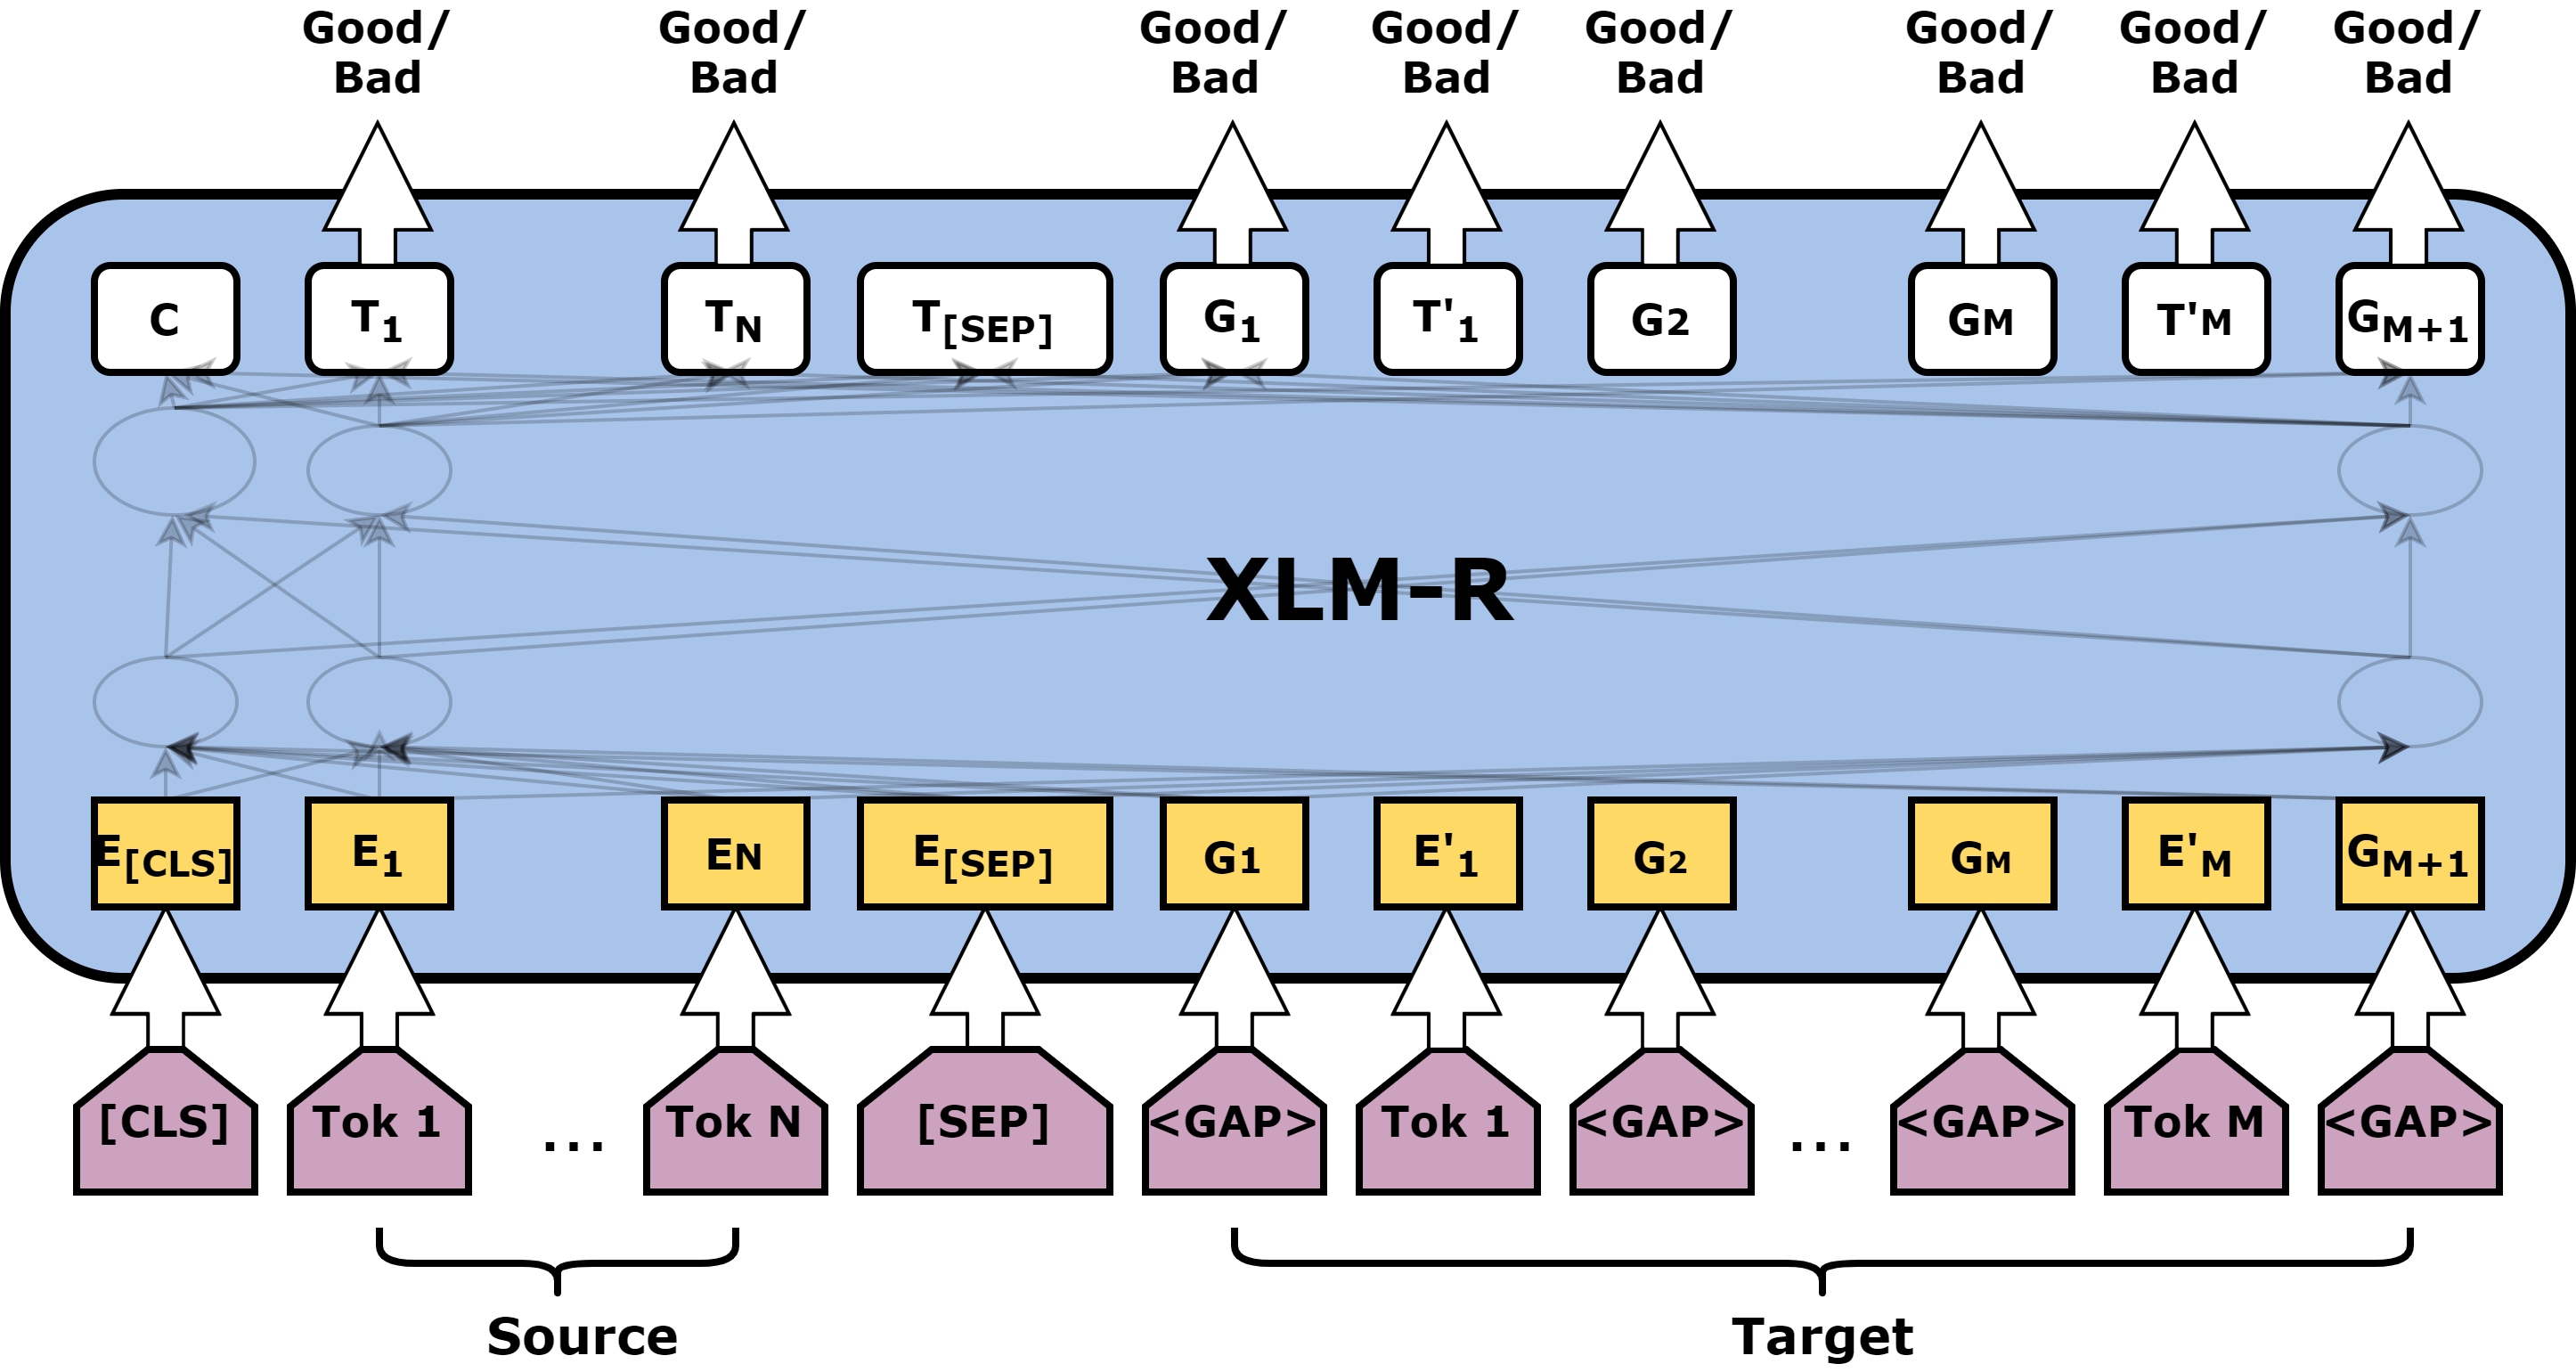
\includegraphics[scale=0.7]{figures/translation_quality_estimation/word_level/MicroTransQuest.png}
	\caption{MicroTransQuest Architecture}
	\label{fig:word_level_architecture}
\end{figure}

\subsection{Experimental Setup}
\label{sec:word_level_experiment}
We evaluated the architecture in word-level quality estimation using the data introduced in Chapter \ref{cha:qe_introduction}. We applied the same set of configurations for all the language pairs in order to ensure consistency between all the experiments. This also provides a good starting configuration for researchers who intend to use MicroTransQuest on a new language pair. We used a batch-size of eight, Adam optimiser with learning rate $1\mathrm{e}{-5}$, and a linear learning rate warm-up over 10\% of the training data. During the training process, the parameters of XLM-R model, as well as the parameters of the subsequent layers, were updated. The models were trained using only training data. Furthermore, they were evaluated while training once in every 300 training steps using an evaluation set that had one fifth of the rows in training data. We performed early stopping if the evaluation loss did not improve over ten evaluation steps. All the models were trained for three epochs.

\section{Results and Evaluation}
\label{sec:word_level_results}
For evaluation, we used the approach proposed in the WMT shared tasks in which the classification performance is calculated using the multiplication of F1-scores (F1-Multi) for the `OK' and `BAD' classes against the true labels
independently: words in the target (`OK' for correct words, `BAD' for incorrect words), gaps in the target (`OK' for genuine gaps, `BAD' for gaps indicating missing words) and source words (`BAD' for words that lead to errors in the target, `OK' for other words) \cite{specia-etal-2018-findings} as we explained in Chapter \ref{cha:qe_introduction} in Part III of the thesis. In WMT QE shared tasks, Word-level QE systems have been evaluated using all three of these evaluation metrics. Therefore, we follow the same process so that we can compare our results with the baselines and best systems of the respective shared task.

F1-Multi for words in target (F1-Multi Target), F1-Multi for gaps in the target (F1-Multi GAPS) and F1-Multi for words in source (F1-Multi Source) are shown in Tables \ref{tab:mt_prediction}, \ref{tab:gap_prediction} and \ref{tab:source_prediction} respectively. Prior to WMT 2019, organisers provided separate scores for gaps and words in the target, while after WMT 2019 they produce a single result for target gaps and words. Therefore, we report "F1-Multi GAPS" only on the language pairs released in WMT 2018 in Table \ref{tab:gap_prediction}. For the language pairs in WMT 2019 and 2020 we report a single result for target gaps and words as (F1-Multi Target) in Table \ref{tab:mt_prediction}.

\renewcommand{\arraystretch}{1.2}
\begin{table}[t]
	\begin{center}
		\small
		% \footnotesize
		\scalebox{0.8}{
			\begin{tabular}{l l  c c c c c c c c} 
				%\hline
				\toprule
				& & \multicolumn{4}{c}{\bf Mid-resource} & \multicolumn{4}{c}{\bf High-resource}\\\cmidrule(r){3-6}\cmidrule(r){7-10}
				&{\bf Method} & \makecell{En-Cs \\ SMT} & \makecell{ En-Ru \\ NMT} & \makecell{En-Lv \\ SMT} & \makecell{En-Lv \\ NMT} & \makecell{De-En \\ SMT} & \makecell{En-Zh \\ NMT} & \makecell{En-De \\ SMT } & \makecell{En-De \\ NMT} \\
				\midrule
				\multirow{1}{*}{\bf I} & MicroTransQuest & 0.6081 & 0.5592 & 0.5939 & 0.5868 & 0.6485 & 0.5602 & 0.6348 & 0.5013\\
				\midrule
				\multirow{1}{*}{\bf II} & MicroTransQuest-base & 0.5642 & 0.5132 & 0.5579 & 0.5431 & 0.6001 & 0.5202 & 0.5985 & 0.4698 \\
				\midrule
				\multirow{1}{*}{\bf III} & MicroTransQuest $\otimes$ & \textbf{0.6154} & \textbf{0.5672} & \textbf{0.6123} & \textbf{0.6003} & \textbf{0.6668} & 0.5678 & \textbf{0.6451} & 0.5121 \\
				\midrule
				\multirow{3}{*}{\bf IV} & Marmot & 0.4449 & NR & 0.3445 & 0.4208 & 0.4373 & NR & 0.3653 & NR \\
				& OpenKiwi & NR & 0.2412 & NR & NR & NR & 0.5583 & NR & 0.4111 \\
				& Best system & 0.4449 & 0.4780 & 0.3618 & 0.4293 & 0.6012 & \textbf{0.6415} & 0.6246 &  \textbf{0.6186} \\
				\midrule
				\multirow{1}{*}{\bf V} & MicroTransQuest-B & 0.5462 & 0.4987 & 0.5043 & 0.5132 & 0.5643 & 0.4892 & 0.5381 & 0.4371 \\
				\bottomrule
				%\bottomrule
			\end{tabular}
		}
	\end{center}
	\caption[F1-Multi Target between the algorithm predictions and human annotations]{F1-Multi Target between the algorithm predictions and human annotations. Best results for each language by any method are marked in bold. Row I shows the results for XLM-R-large model and Row II shows the results for XLM-R-base. Row III presents the results for further fine-tuning strategies explained in Section \ref{sec:word_level_further}. Row IV shows the results of the baseline methods and the best system submitted for the language pair in that competition. \textbf{NR} implies that a particular result was \textit{not reported} by the organisers. Row V presents the results of the multilingual BERT (mBERT) model in MicroTransQuest.} 
	\label{tab:mt_prediction}
\end{table}


\renewcommand{\arraystretch}{1.2}
\begin{table}[t]
	\begin{center}
	\small
	% \footnotesize
	\scalebox{1.0}{
		\begin{tabular}{l l  c c c c c } 
			%\hline
			\toprule
			& & \multicolumn{3}{c}{\bf Mid-resource} & \multicolumn{2}{c}{\bf High-resource}\\\cmidrule(r){3-5}\cmidrule(r){6-7}
			&{\bf Method} & \makecell{En-Cs \\ SMT} & \makecell{En-Lv \\ SMT} & \makecell{En-Lv \\ NMT} & \makecell{De-En \\ SMT}  & \makecell{En-De \\ SMT }  \\
			\midrule
			\multirow{1}{*}{\bf I} & MicroTransQuest & 0.2018 & 0.2356 & 0.1664 & 0.4203 & 0.4927 \\
			\midrule
			\multirow{1}{*}{\bf II} & MicroTransQuest-base & 0.1876 & 0.2132 & 0.1452 & 0.4098 & 0.4679 \\
			\midrule
			\multirow{1}{*}{\bf III} & MicroTransQuest $\otimes$ & \textbf{0.2145} & \textbf{0.2437} & \textbf{0.1764} & \textbf{0.4379} & \textbf{0.4982} \\
			\midrule
			\multirow{2}{*}{\bf IV} & Marmot & NS & NS & NS & NS & NS   \\
			& Best system & 0.1671 & 0.1386 & 0.1598 & 0.3176 & 0.3161  \\
			\midrule
			\multirow{1}{*}{\bf V} & MicroTransQuest-B & 0.1778 & 0.2089 & 0.1387 & 0.3892 & 0.4371  \\
			\bottomrule
			%\bottomrule
		\end{tabular}
	}
\end{center}
	\caption[F1-Multi GAPS between the algorithm predictions and human annotations]{F1-Multi GAPS between the algorithm predictions and human annotations. Best results for each language by any method are marked in bold. Row I shows the results for XLM-R-large model and Row II shows the results for XLM-R-base. Row III presents the results for further fine-tuning strategies explained in Section \ref{sec:word_level_further}. Row IV shows the results of the baseline methods and the best system submitted for the language pair in that competition. \textbf{NS} implies that a particular baseline does \textit{not support} predicting quality of gaps. Row V presents the results of the multilingual BERT (mBERT) model in MicroTransQuest.} 
	\label{tab:gap_prediction}
\end{table}


\renewcommand{\arraystretch}{1.2}
\begin{table}[t]
	\begin{center}
		\small
		% \footnotesize
		\scalebox{0.8}{
			\begin{tabular}{l l  c c c c c c c c} 
				%\hline
				\toprule
				& & \multicolumn{4}{c}{\bf Mid-resource} & \multicolumn{4}{c}{\bf High-resource}\\\cmidrule(r){3-6}\cmidrule(r){7-10}
				&{\bf Method} & \makecell{En-Cs \\ SMT} & \makecell{ En-Ru \\ NMT} & \makecell{En-Lv \\ SMT} & \makecell{En-Lv \\ NMT} & \makecell{De-En \\ SMT} & \makecell{En-Zh \\ NMT} & \makecell{En-De \\ SMT } & \makecell{En-De \\ NMT} \\
				\midrule
				\multirow{1}{*}{\bf I} & MicroTransQuest & 0.5327 & 0.5543 & 0.4945 & 0.4880 & 0.4824 & 0.4040 & 0.5269 & 0.4456\\
				\midrule
				\multirow{1}{*}{\bf II} & MicroTransQuest-base & 0.5134 & 0.5287 & 0.4652 & 0.4571 & 0.4509 & 0.3876 & 0.5012 & 0.4185 \\
				\midrule
				\multirow{1}{*}{\bf III} & MicroTransQuest $\otimes$ & \textbf{0.5431} & \textbf{0.5640} & \textbf{0.5076} & \textbf{0.4892} & \textbf{0.4965} & 0.4145 & \textbf{0.5387} & 0.4578 \\
				\midrule
				\multirow{3}{*}{\bf IV} & Marmot & NS & NR & NS & NS & NS & NR & NS & NR \\
				& OpenKiwi & NR & 0.2647 & NR & NR & NR & 0.3729 & NR & 0.3717 \\
				& Best system & 0.3937 & 0.4541 & 0.4945 & 0.3614 & 0.3200 & \textbf{0.4462} & 0.3368 &  \textbf{0.5672} \\
				\midrule
				\multirow{1}{*}{\bf V} & MicroTransQuest-B & 0.4987 & 0.5098 & 0.4441 & 0.4256 & 0.4187 & 0.3567 & 0.4672 & 0.3985 \\
				\bottomrule
				%\bottomrule
			\end{tabular}
		}
	\end{center}
	\caption[F1-Multi Source between the algorithm predictions and human annotations]{F1-Multi Source between the algorithm predictions and human annotations. Best results for each language by any method are marked in bold. Row I shows the results for XLM-R-large model and Row II shows the results for XLM-R-base. Row III presents the results for further fine-tuning strategies explained in Section \ref{sec:word_level_further}. Row IV shows the results of the baseline methods and the best system submitted for the language pair in that competition. \textbf{NR} implies that a particular result was \textit{not reported} by the organisers. Row V presents the results of the multilingual BERT (mBERT) model in MicroTransQuest.} 
	\label{tab:source_prediction}
\end{table}

 Raw I in Tables \ref{tab:mt_prediction}, \ref{tab:gap_prediction} and \ref{tab:source_prediction} shows the results for MicroTransQuest with XLM-R-large and Raw II in Tables  \ref{tab:mt_prediction}, \ref{tab:gap_prediction} and \ref{tab:source_prediction} shows the results for MicroTransQuest with XLM-R-base. As can be seen in results XLM-R-large always outperformed XLM-R-base. Therefore, we use the results we got from XLM-R-large for the following analysis.
 
 In F1-Multi Target evaluation metric in word-level QE, as shown in Table \ref{tab:mt_prediction}, \textit{MicroTransQuest} outperforms OpenKiwi and Marmot in all the language pairs we experimented. Additionally, \textit{MicroTransQuest} achieves $\approx$ 0.3 F1-Multi score boost over OpenKiwi in the En-Ru NMT. Furthermore, \textit{MicroTransQuest} gained $\approx$ 0.15-0.2 F1-Multi score boost over Marmot in all the language pairs. Table \ref{tab:mt_prediction}  also gives the results of the best system submitted for a particular language pair. It is worth noting that the \textit{MicroTransQuest} results surpass the best system in all the language pairs with the exception of the En-De NMT and En-Zh NMT datasets.
 
 In F1-Multi GAP evaluation metric in word-level QE, as shown in Table \ref{tab:gap_prediction} \textit{MicroTransQuest} outperforms best systems submitted to the respective shared tasks in all the language pairs we experimented. \textit{MicroTransQuest} achieves $\approx$ 0.05-0.2 F1-Multi score boost over best systems. Notably \textit{MicroTransQuest} achieves $\approx$ 0.2 F1-Multi score boost over the best system in En-De SMT. As we mentioned before, it should be noted that neither of the baselines; Marmot nor OpenKiwi supports predicting the quality of \textit{gaps} in target sentence. Since \textit{MicroTransQuest} supports this and produces state-of-the-results in this evaluation metric too, we believe that using \textit{MicroTransQuest} in word-level QE would be beneficial than using OpenKiwi and Marmot.
 
Finally in F1-Multi Source evaluation metric too, as shown in Table \ref{tab:source_prediction} \textit{MicroTransQuest} outperforms OpenKiwi in all the language pairs we experimented. It should be noted that Marmot does not support predicting the quality of the words in source. On the other hand, OpenKiwi supports this, but still \textit{MicroTransQuest} achieves $\approx$ 0.05-0.3 F1-Multi score boost in all the language pairs. Furthermore, \textit{MicroTransQuest} results surpass the best system in all the language pairs with the exception of the En-De NMT and En-Zh NMT datasets.

With these results we can answer our \textbf{RQ1:} Can existing state-of-the-art STS architecture be used to predict all features in word-level QE task by just modifying the embeddings and the output layer? We show that state-of-the-art STS method based on crosslingual transformer models can be used in word-level QE too by just changing the output layer and it outperforms current state-of-the-art word-level QE methods like OpenKiwi that relies on complex neural network architectures. Our proposed architecture is not only simple, but also achieves state-of-the-art results in all the language pairs we experimented. Furthermore, \textit{MicroTransQuest} is the only architecture that supports predicting the quality of the gaps in target. We believe that the way we designed the architecture based on state-of-the-art STS architectures gave us the ability to support predicting the quality of the gaps in target with \textit{MicroTransQuest}.

Row VI in Tables \ref{tab:mt_prediction}, \ref{tab:gap_prediction} and \ref{tab:source_prediction} shows the results of multilingual BERT (mBERT) in MicroTransQuest architecture. We used the same settings similar to XLM-R. The results show that XLM-R model outperforms the mBERT model in all the language pairs. As shown in row II in Tables \ref{tab:mt_prediction}, \ref{tab:gap_prediction} and \ref{tab:source_prediction} even XLM-R-base model outperform mBERT model in all the languages pairs. Therefore, we can safely assume that the cross lingual nature of the XLM-R transformers had a clear impact to the results. This observation is similar to what we experienced in Chapter \ref{cha:qe_transquest} with sentence-level QE experiments.

With this we can answer our \textbf{RQ2:} Using crosslingual embeddings with STS architecture proved advantageous rather than using just multilingual embeddings. As far as we know, this is the first time XLM-R was used in a task related to detecting missing words. With the results we got from predicting quality of the gaps in target, we show that XLM-R can be used in tasks similar to detecting missing words too.
 

\section{Further Improvements}
\label{sec:word_level_further}
In this section. we try improve the results of MicroTransQuest through ensemble learning as we did with sentence-level quality estimation. As me mentioned before in Section \ref{sec:word_level_method} softmax layer provides two probabilities for each word or gap. We calculated these probabilities for each word using XLM-R-large and XLM-R base. Then we performed a weighted average ensemble on these probabilities and we consider the class with highest probability after performing the ensemble as the quality of the word or gap. We experimented on weights 0.8:0.2, 0.6:0.4, 0.5:0.5 on the output of XLM-R-large and output from XLM-R-base respectively. Since the results we got from XLM-R-base transformer model are slightly worse than the results we got from XLM-R-large we did not consider the weight combinations that gives higher weight to XLM-R-base transformer model results. We obtained best results when we used the weights 0.6:0.4. We report the results from this step in row III of Tables \ref{tab:mt_prediction}, \ref{tab:gap_prediction} and \ref{tab:source_prediction} as MicroTransQuest $\otimes$.

As shown in Tables \ref{tab:mt_prediction}, \ref{tab:gap_prediction} and \ref{tab:source_prediction} ensemble learning improved the results for \textit{MicroTransQuest} in all three evaluation metrics. For all the language pairs F1 Multi Target, F1 Multi GAPS and F1 Multi Source scores gained $\approx$ 0.01-0.02 boost with ensemble learning. This answers our \textbf{RQ3:} Can the proposed model further improved by performing ensemble learning? We show that ensemble learning can be used to improve the word-level QE results similar to sentence-level QE. In fact, ensemble learning provided the best results for MicroTransQuest in all the language pairs we experimented.

\section{Conclusion}
In this chapter, we explored word-level QE with transformers. We introduced a new architecture based on transformers to perform word-level QE. The proposed architecture is very similar to the sentence-level QE architecture; \textit{MonoTransQuest}. However, the output layers are different to \textit{MonoTransQuest} so that they keep the state of the individual tokens to get their quality. We evaluated the proposed architecture; \textit{MicroTransQuest} on eight language pairs where the QE data was available.  It outperforms other open-source tools like OpenKiwi and Marmot on all three evaluations metrics of word-level quality estimation and yields new state-of-the-art word-level QE results. Furthermore, \textit{MicroTransQuest} is the only open source architecture that supports predicting the quality of the gaps in target sentence. The architecture we proposed in this Chapter is very simple when compared with the predictor-estimator architecture in OpenKiwi, yet this architecture produce better results. We further improved the results with ensemble learning showed that \textit{MicroTransQuest} outperforms majority of the best systems submitted for that language in each shared task. We can conclude that state-of-the-art STS architecture can be used in word-level QE too by doing small modifications to the output layers.

The implementation of the architecture, which is based on PyTorch \cite{NEURIPS2019_9015} and Hugging Face \cite{wolf-etal-2020-transformers}, has been integrated into the TransQuest framework \cite{ranasinghe-etal-2020-transquest} which won the WMT 2020 QE task \cite{specia-etal-2020-findings-wmt} on sentence-level direct assessment \cite{ranasinghe-etal-2020-transquest-wmt2020}\footnote{The details about the word-level QE architecture in TransQuest is available on \url{http://tharindu.co.uk/TransQuest/architectures/word_level_architecture/}}. The pre-trained word-level QE models for eight language pairs are available to the public on HuggingFace model hub. 

One limitation of the proposed architecture is that it only predicts word-level qualities. Managing two models to predict word-level and sentence-level qualities separately would be chaotic in some situations. Therefore, in the future we hope to explore multi-task learning for word-level and sentence-level QE \cite{Caruana1997}. The two tasks are related as word-level quality contributes to the sentence-level quality in general. Therefore we believe that a multi-task architecture that can learn both tasks at the same time can be advantageous. 

As we discussed at multiple points in this thesis, pre-trained models based on transformers are big in size. Therefore, managing a several of them for each language pair would be chaotic in a real-world application for word-level QE too. As a solution for that we explore multilingual word-level QE models in Chapter \ref{cha:qe_multilingual} in Part III of the thesis.




\newcommand\figlength{6cm}

\chapter{\label{cha:qe_multilingual}Multilingual Quality Estimation with TransQuest}

Machine translation quality estimation is traditionally framed as a supervised machine learning problem \autocite{kepler-etal-2019-openkiwi,lee-2020-two} where the machine learning models are trained on language specific data for quality estimation. We refer to these models as bilingual QE models. This process would require having annotated QE data for all the language pairs. Furthermore, this language specific supervised machine learning process would result in having machine learning models for each language pair separately. 

This traditional approach has obvious drawbacks. As mentioned before, this process requires training data for each language pair. However, the training data publicly available to build QE models is limited to very few language pairs, making it difficult to build QE models for many languages. Furthermore, from an application perspective, even for the languages with resources, it is difficult to maintain separate QE models for each language since the state-of-the-art neural QE models are large in size \autocite{ranasinghe-etal-2020-transquest}. 

To understand this scale, consider a real-world application where it is required to build a quality estimation solution for the European Parliament. The European Parliament has 24 languages, resulting in 24*23 language pairs equal to 552 language pairs. A traditional bilingual QE solution would require 552 training datasets to train the models, which is highly challenging and costly to collect and annotate. Furthermore, this would require having 552 machine learning models. State-of-the-art QE models like TransQuest are at least 2GB in size. Having 2GB sized 552 models in the RAM at inferencing time would not be practical. The solution to all these problems is Multilingual QE models. 

Multilingual models allow training a single model to perform a task from and/or to multiple languages. Even though multilingual learning has been applied to many tasks \autocite{ranasinghe-zampieri-2020-multilingual,ranasinghe-zampieri-2021-mudes} including NMT \autocite{nguyen-chiang-2017-transfer, aharoni-etal-2019-massively}, multilingual approaches have been rarely used in QE \autocite{sun-etal-2020-exploratory}. Therefore, in this chapter we explore multilingual models with the \textit{TransQuest} architectures we introduced in Chapters \ref{cha:qe_transquest} and \ref{cha:qe_word} for sentence-level QE and word-level QE respectively. Since we used a cross-lingual transformer model that supports 104 languages \autocite{conneau-etal-2020-unsupervised} it is possible to explore multilingual learning with the same setup.


Usually, the neural machine learning models are \textit{hungry for data}. They need a lot of annotated data for the training process, which is a challenge for the low resource languages. Recently, researchers are trying to exploit this behaviour with learning paradigms such as few-shot and zero-shot learning.  What we define as few-shot learning in this chapter is the process where the QE model only sees a few instances from a certain language pair in the training process \autocite{10.1145/3386252} while in zero-shot learning, QE model would not see any instances from a certain language pair \autocite{10.5555/1620163.1620201} in the training process. Even though few-shot and zero-shot learning has been popular in machine learning applications, including NLP, they have not been explored with QE. Exploring them would benefit the low resource languages, which the QE training data is difficult to find. Therefore, this chapter inspects how the bilingual and multilingual QE models behave in few-shot and zero-shot learning environments.


As far as we know, this is the first study done on multilingual word-level and sentence-level QE. We address three research questions in this chapter:

\textbf{RQ1:} Do multilingual models based on existing state-of-the-art sentence-level, and word-level QE architectures perform competitively with the related bilingual models?

\textbf{RQ2:} How do the bilingual and multilingual models perform in a zero-shot environment, and what is the impact of source-target direction, domain and MT type for zero-shot learning?

\textbf{RQ3:} Do multilingual QE models perform better with a limited number of training instances (Few-shot learning) for an unseen language pair?


The main contributions of this Chapter are, 

\begin{enumerate}

\item We explore multilingual, sentence-level and word-level quality estimation with the proposed architectures in \textit{TransQuest}. We show that multilingual models are competitive with bilingual models.

\item We inspect few-shot and zero-shot sentence-level and word-level quality estimation with the bilingual and multilingual models. We report how the source-target direction, domain and MT type affect the predictions for a new language pair.

\item The code and the pre-trained multilingual models of \textit{TransQuest} are publicly available to the community\footnote{The pre-trained multilingual QE models are available on the HuggingFace model repository on \url{https://huggingface.co/TransQuest}}.

\end{enumerate} 

The rest of this chapter is organised as follows. Section \ref{sec:multilingual_method} discusses the methodology and the multilingual experiments done with 15 language pairs in sentence-level QE and word-level QE.  Section \ref{sec:multilingual_results} shows the results and Sections \ref{sec:multilingual_zeroshot} and \ref{sec:multilingual_fewshot} provide further analysis on zero-shot and few-shot learning. The chapter finishes with conclusions and ideas for future research directions in multilingual QE.
 

\section{Methodology}
\label{sec:multilingual_method}
As mentioned before, we conducted the experiments with the architectures explored in Chapters \ref{cha:qe_transquest} and \ref{cha:qe_word}. For the multilingual sentence-level experiments, we used the \textit{MonoTransQuest} architecture introduced in Chapter \ref{cha:qe_transquest} which outperformed other open-source QE frameworks and best systems submitted to the shared tasks in the majority of the language pairs. We experimented with both aspects of sentence-level QE, HTER and DA with all the datasets introduced in Chapter \ref{cha:qe_introduction}. For the word-level experiments, we used the \textit{MicroTransQuest} architecture which again outperformed other open-source QE frameworks and best systems submitted to the shared tasks in the majority of the language pairs in word-level QE. As the word-level QE data, we considered all the word-level QE datasets introduced in Chapter \ref{cha:qe_introduction}.

For the experiments, we considered XLM-R large model and did not use the ensemble models to keep the multilingual experiments simpler. We applied the same set of configurations for all the training processes to ensure consistency between the experiments. We used a batch size of eight, Adam optimiser and a linear learning rate warm-up over 10\% of the training data. During the training process, the parameters of the XLM-R-large model, as well as the parameters of the subsequent layers, were updated. The models were trained using only training data. Furthermore, they were evaluated while training once in every 100 training steps using an evaluation set with one-fifth of the training data rows. We performed early stopping if the evaluation loss did not improve over ten evaluation steps. All the models were trained for three epochs. We used a learning rate of $2\mathrm{e}^{-5}$ for the sentence-level experiments while for word-level experiments it was $1\mathrm{e}^{-5}$. 



\section{Results}
\label{sec:multilingual_results}
In the following sections, we explore different multilingual QE settings and compare the multilingual results to the results we got with supervised, bilingual QE models. 

For the sentence-level evaluations, we used Pearson correlation, the same evaluation metric we used for bilingual sentence-level QE in Chapter \ref{cha:qe_transquest}, which was used for WMT QE shared tasks. Results for multilingual sentence-level QE experiments with HTER and DA are shown in Tables \ref{tab:multilingual_hter} and \ref{tab:multilingual_direct_assesement}. For the word-level evaluations, we used the same evaluation metrics we used for bilingual word-level QE in Chapter \ref{cha:qe_word} which in turn was used for the WMT QE shared tasks. Results for multilingual word-level QE experiments with regards to $F1_{\textit{MULTI}}$ for words in target ($F1_{\textit{MULTI}} \; Target$), $F1_{\textit{MULTI}}$ for gaps in the target ($F1_{\textit{MULTI}} \; GAPS$) and $F1_{\textit{MULTI}}$ for words in source ($F1_{\textit{MULTI}} \; Source$) are shown in Tables \ref{tab:multilingual_mt_prediction}, \ref{tab:multilingual_gap_prediction} and \ref{tab:multilingual_source_prediction} respectively. 


The values displayed diagonally across the Row I of Tables  \ref{tab:multilingual_hter}, \ref{tab:multilingual_direct_assesement}, \ref{tab:multilingual_mt_prediction}, \ref{tab:multilingual_gap_prediction} and \ref{tab:multilingual_source_prediction} show the results for supervised, bilingual, QE models where the model was trained on the training set of a particular language pair and tested on the test set of the same language pair. This is the exact result we reported in the Row I of Tables \ref{tab:hter_prediction}, \ref{tab:da_prediction}, \ref{tab:mt_prediction}, \ref{tab:gap_prediction} and \ref{tab:source_prediction} in Chapters \ref{cha:qe_transquest} and \ref{cha:qe_word}, which we got with \textit{MonoTransQuest} and \textit{MicroTransQuest} using  XLM-R-large model \autocite{conneau-etal-2020-unsupervised} for sentence-level and word-level. 

\renewcommand{\arraystretch}{1.2}
\begin{table}[t]
	\begin{center}
		\small
		\scalebox{0.77}{
			% \footnotesize
			\begin{tabular}{l l c c c c c c c c} 
				%\hline
				\toprule
				& & \multicolumn{3}{c}{\bf IT} & \multicolumn{3}{c}{\bf Pharmaceutical} & \multicolumn{2}{c}{\bf Wiki}\\
				\cmidrule(r){3-5}\cmidrule(r){6-8}\cmidrule(r){9-10}
				&{\bf \makecell{Train \\ Language(s)} } & \makecell{En-Cs \\ SMT}  & \makecell{En-De \\ SMT} & \makecell{En-Ru \\ NMT} & \makecell{De-En \\ SMT} & \makecell{En-LV \\ NMT} & \makecell{En-Lv \\ SMT } & \makecell{En-De \\ NMT} & \makecell{En-Zh \\ NMT} \\
				\midrule
				\multirow{8}{*}{\bf I} & En-Cs SMT & \textbf{0.7207} & \textcolor{gray}{(-0.06)} & \textcolor{gray}{(-0.07)} & \textcolor{gray}{(-0.13)} & \textcolor{gray}{(-0.02)} & \textcolor{gray}{(-0.01)} & \textcolor{gray}{(-0.11)} &  \textcolor{gray}{(-0.10)}\\
				& En-De SMT & \textcolor{gray}{(-0.01)} &  0.7137 & \textcolor{gray}{(-0.04)} & \textcolor{gray}{(-0.12)} & \textcolor{gray}{(-0.04)} & \textcolor{gray}{(-0.05)} & \textcolor{gray}{(-0.07)} &  \textcolor{gray}{(-0.07)} \\
				& En-Ru NMT & \textcolor{gray}{(-0.12)} &  \textcolor{gray}{(-0.15)} & \textbf{0.7126} & \textcolor{gray}{(-0.13)} & \textcolor{gray}{(-0.01)} & \textcolor{gray}{(-0.02)} & \textcolor{gray}{(-0.08)} & \textcolor{gray}{(-0.07)} \\
				& De-En SMT & \textcolor{gray}{(-0.39)} &  \textcolor{gray}{(-0.29)} & \textcolor{gray}{(-0.34)} & \textbf{0.7939} & \textcolor{gray}{(-0.27)} & \textcolor{gray}{(-0.31)} & \textcolor{gray}{(-0.26)} & \textcolor{gray}{(-0.27)} \\
				& En-LV NMT & \textcolor{gray}{(-0.11)} &  \textcolor{gray}{(-0.13)} & \textcolor{gray}{(-0.02)} & \textcolor{gray}{(-0.11)} & 0.7394 & \textcolor{gray}{(-0.01)} & \textcolor{gray}{(0.08)} & \textcolor{gray}{(-0.07)} \\
				& En-Lv SMT & \textcolor{gray}{(-0.03)} &  \textcolor{gray}{(-0.09)} & \textcolor{gray}{(-0.08)} & \textcolor{gray}{(-0.15)} & \textcolor{gray}{(-0.01)}  & 0.6592 & \textcolor{gray}{(-0.13)} & \textcolor{gray}{(-0.13)} \\
				& En-De NMT & \textcolor{gray}{(-0.11)} &  \textcolor{gray}{(-0.07)} & \textcolor{gray}{(-0.02)} & \textcolor{gray}{(-0.12)} & \textcolor{gray}{(-0.01)}  & \textcolor{gray}{(-0.02)} & 0.5994 &  \textcolor{gray}{(-0.04)} \\
				& En-Zh NMT & \textcolor{gray}{(-0.21)} &  \textcolor{gray}{(-0.18)} & \textcolor{gray}{(-0.02)} & \textcolor{gray}{(-0.18)} & \textcolor{gray}{(-0.02)}  & \textcolor{gray}{(-0.07)} & \textcolor{gray}{(-0.08)} & 0.6119 \\
				\midrule
				\multirow{2}{*}{\bf II} & All & 0.7111 &  \textbf{0.7300} & 0.7012 & 0.7878 & \textbf{0.7450} & \textbf{0.7141} & 0.5982 & 0.6092\\
				& All-1 & \textcolor{gray}{(-0.01)} &  \textcolor{gray}{(-0.04)} & \textcolor{gray}{(-0.02)} & \textcolor{gray}{(-0.11)} & \textcolor{gray}{(-0.01)} & \textcolor{gray}{(-0.01)} & \textcolor{gray}{(-0.01)} & \textcolor{gray}{(-0.03)} \\
				\midrule
				\multirow{1}{*}{\bf III} & Domain & 0.7001 &  0.7256 & 0.6987 & 0.7754 & 0.7412 & 0.7065  & 0.5764 &  0.5671 \\
				\midrule
				\multirow{1}{*}{\bf IV} & SMT/NMT & 0.6998 &  0.7143 & 0.6998 & 0.7642 & 0.7319 & 0.6872 & 0.5671 & 0.5601 \\
				\midrule
				\multirow{3}{*}{\bf V} & Quest++ & 0.3943 &  0.3653 & NR & 0.3323 & 0.4435 & 0.3528 & NR & NR \\
				& OpenKiwi & NR &  NR & 0.5923 & NR & NR & NR & 0.3923 & 0.5058 \\
				& Best system & 0.6918 &  0.7397 & 0.5923 & 0.7888 & 0.6819 & 0.6188 & \textbf{0.7582} & \textbf{0.6641} \\
				\bottomrule
				%\bottomrule
			\end{tabular}
		}
	\end{center}
\caption[Pearson correlation between the MonoTransQuest predictions and human post-editing effort in multilingual experiments]{Pearson correlation ($\bm{\rho}$) between the \textit{MonoTransQuest} predictions and human post-editing effort in multilingual experiments. The best result for each language by any method is highlighted in bold. Rows \textbf{I}, \textbf{II}, \textbf{III} and \textbf{IV} indicate the different multilingual settings. Row \textbf{V} shows the results of the baselines and the best system submitted for the language pair in that competition. \textbf{NR} implies that a particular result was \textit{not reported} by the organisers. Zero-shot results are coloured in grey and the value shows the difference between the best result in that Row for that language pair and itself.} 
	\label{tab:multilingual_hter}
\end{table}


\renewcommand{\arraystretch}{1.2}
\begin{table*}[t]
	\begin{center}
		\small
		% \footnotesize
		\begin{tabular}{l l  c c c c c c c} 
			%\hline
			\toprule
			& & \multicolumn{2}{c}{\bf Low-resource} & \multicolumn{3}{c}{\bf Mid-resource} & \multicolumn{2}{c}{\bf High-resource}\\\cmidrule(r){3-4}\cmidrule(lr){5-7}\cmidrule(l){8-9}
			&{\bf \makecell{Train \\ Language(s)} } & Si-En & Ne-En & Et-En & Ro-En & Ru-En & En-De & En-Zh\\
			\midrule
			\multirow{7}{*}{\bf I} & Si-En & 0.6525 & \textcolor{gray}{(-0.05)} & \textcolor{gray}{(-0.08)} & \textcolor{gray}{(-0.15)} & \textcolor{gray}{(-0.07)} & \textcolor{gray}{(-0.13)} & \textcolor{gray}{(-0.13)} \\
			& Ne-En & \textcolor{gray}{(-0.10)} & 0.7914 & \textcolor{gray}{(-0.06)}  & \textcolor{gray}{(-0.08)} & \textcolor{gray}{(-0.08)} & \textcolor{gray}{(-0.10)} & \textcolor{gray}{(-0.11)} \\
			& Et-En & \textcolor{gray}{(-0.07)} & \textcolor{gray}{(-0.10)} & 0.7748 &  \textcolor{gray}{(-0.20)} & \textcolor{gray}{(-0.08)} & \textcolor{gray}{(-0.10)} & \textcolor{gray}{(-0.08)} \\
			& Ro-En & \textcolor{gray}{(-0.02)} & \textcolor{gray}{(-0.04)} & \textcolor{gray}{(-0.02)} & \textbf{0.8982} & \textcolor{gray}{(-0.08)} & \textcolor{gray}{(-0.10)} & \textcolor{gray}{(-0.14)} \\
			& Ru-En & \textcolor{gray}{(-0.11)}  & \textcolor{gray}{(-0.16)} & \textcolor{gray}{(-0.19)} & \textcolor{gray}{(-0.26)} & 0.7734 & \textcolor{gray}{(-0.04)} & \textcolor{gray}{(-0.09)} \\
			& En-De & \textcolor{gray}{(-0.32)} & \textcolor{gray}{(-0.51)} & \textcolor{gray}{(-0.39)} & \textcolor{gray}{(-0.51)} & \textcolor{gray}{(-0.35)} & \textbf{0.4669} & \textcolor{gray}{(-0.17)} \\
			& En-Zh & \textcolor{gray}{(-0.16)} & \textcolor{gray}{(-0.24)} & \textcolor{gray}{(-0.19)} & \textcolor{gray}{(-0.36)} & \textcolor{gray}{(-0.17)} & \textcolor{gray}{(-0.02)} & \textbf{0.4779} \\
			\midrule
			\multirow{2}{*}{\bf II} & All &  0.6526 & 0.7581 & 0.7574 & 0.8856  &  0.7521 &  0.4420 &  0.4646 \\
			& All-1 & \textcolor{gray}{(-0.02)} & \textcolor{gray}{(-0.02)} & \textcolor{gray}{(-0.02)} & \textcolor{gray}{(-0.03)} & \textcolor{gray}{(-0.02)} & \textcolor{gray}{(-0.02)} &  \textcolor{gray}{(-0.05)} \\
			\midrule
			\multirow{1}{*}{\bf III} & OpenKiwi & 0.3737 & 0.3860 & 0.4770 & 0.6845 & 0.5479 & 0.1455 & 0.1902 \\
			
			\bottomrule
		\end{tabular}
	\end{center}
	\caption[Pearson correlation between the MonoTransQuest predictions and human DA judgments in multilingual experiments]{Pearson correlation ($\bm{\rho}$) between the \textit{MonoTransQuest} predictions and human DA judgments in multilingual experiments. The best result for each language by any method is highlighted in bold. Rows \textbf{I} and \textbf{II} indicate the different multilingual settings. Row \textbf{III} shows the results of the baselines and the best system submitted for the language pair in that competition. Zero-shot results are coloured in grey and the value shows the difference between the best result in that Row for that language pair and itself. }
	\label{tab:multilingual_direct_assesement}
\end{table*}


\renewcommand{\arraystretch}{1.2}
\begin{table}[t]
	\begin{center}
		\small
		\scalebox{0.77}{
			% \footnotesize
			\begin{tabular}{l l c c c c c c c c} 
				%\hline
				\toprule
				& & \multicolumn{3}{c}{\bf IT} & \multicolumn{3}{c}{\bf Pharmaceutical} & \multicolumn{2}{c}{\bf Wiki}\\
				\cmidrule(r){3-5}\cmidrule(r){6-8}\cmidrule(r){9-10}
				&{\bf \makecell{Train \\ Language(s)} } & \makecell{En-Cs \\ SMT}  & \makecell{En-De \\ SMT} & \makecell{En-Ru \\ NMT} & \makecell{De-En \\ SMT} & \makecell{En-LV \\ NMT} & \makecell{En-Lv \\ SMT } & \makecell{En-De \\ NMT} & \makecell{En-Zh \\ NMT} \\
				\midrule
				\multirow{8}{*}{\bf I} & En-Cs SMT & 0.6081 & \textcolor{gray}{(-0.07)} & \textcolor{gray}{(-0.09)} & \textcolor{gray}{(-0.15)} & \textcolor{gray}{(-0.02)} & \textcolor{gray}{(-0.01)} & \textcolor{gray}{(-0.10)} &  \textcolor{gray}{(-0.11)}\\
				& En-De SMT & \textcolor{gray}{(-0.01)} &  0.6348 & \textcolor{gray}{(-0.07)} & \textcolor{gray}{(-0.14)} & \textcolor{gray}{(-0.06)} & \textcolor{gray}{(-0.04)} & \textcolor{gray}{(-0.06)} &  \textcolor{gray}{(-0.09)} \\
				& En-Ru NMT & \textcolor{gray}{(-0.14)} &  \textcolor{gray}{(-0.16)} & \textbf{0.5592} & \textcolor{gray}{(-0.12)} & \textcolor{gray}{(-0.01)} & \textcolor{gray}{(-0.03)} & \textcolor{gray}{(-0.09)} & \textcolor{gray}{(-0.08)} \\
				& De-En SMT & \textcolor{gray}{(-0.43)} &  \textcolor{gray}{(-0.33)} & \textcolor{gray}{(-0.31)} & \textbf{0.6485} & \textcolor{gray}{(-0.29)} & \textcolor{gray}{(-0.32)} & \textcolor{gray}{(-0.25)} & \textcolor{gray}{(-0.28)} \\
				& En-LV NMT & \textcolor{gray}{(-0.12)} &  \textcolor{gray}{(-0.14)} & \textcolor{gray}{(-0.03)} & \textcolor{gray}{(-0.12)} & 0.5868 & \textcolor{gray}{(-0.01)} & \textcolor{gray}{(0.09)} & \textcolor{gray}{(-0.08)} \\
				& En-Lv SMT & \textcolor{gray}{(-0.04)} &  \textcolor{gray}{(-0.10)} & \textcolor{gray}{(-0.09)} & \textcolor{gray}{(-0.16)} & \textcolor{gray}{(-0.01)}  & 0.5939 & \textcolor{gray}{(-0.15)} & \textcolor{gray}{(-0.14)} \\
				& En-De NMT & \textcolor{gray}{(-0.11)} &  \textcolor{gray}{(-0.08)} & \textcolor{gray}{(-0.02)} & \textcolor{gray}{(-0.14)} & \textcolor{gray}{(-0.02)}  & \textcolor{gray}{(-0.04)} & 0.5013 &  \textcolor{gray}{(-0.06)} \\
				& En-Zh NMT & \textcolor{gray}{(-0.19)} &  \textcolor{gray}{(-0.17)} & \textcolor{gray}{(-0.03)} & \textcolor{gray}{(-0.16)} & \textcolor{gray}{(-0.03)}  & \textcolor{gray}{(-0.06)} & \textcolor{gray}{(-0.07)} & 0.5402 \\
				\midrule
				\multirow{2}{*}{\bf II} & All & \textbf{0.6112} &  \textbf{0.6583} & 0.5558 & 0.6221 & \textbf{0.5991} & \textbf{0.5980} & 0.5101 & 0.5229\\
				& All-1 & \textcolor{gray}{(-0.01)} &  \textcolor{gray}{(-0.05)} & \textcolor{gray}{(-0.02)} & \textcolor{gray}{(-0.12)} & \textcolor{gray}{(-0.01)} & \textcolor{gray}{(-0.01)} & \textcolor{gray}{(-0.01)} & \textcolor{gray}{(-0.05)} \\
				\midrule
				\multirow{1}{*}{\bf III} & Domain & 0.6095 &  0.6421 & 0.5560 & 0.6331 & 0.5892 & 0.5951  & 0.5021 &  0.5210 \\
				\midrule
				\multirow{1}{*}{\bf IV} & SMT/NMT & 0.6092 &  0.6410 & 0.5421 & 0.6320 & 0.5885 & 0.5934 & 0.5010 & 0.5205 \\
				\midrule
				\multirow{3}{*}{\bf V} & Marmot & 0.4449 &  0.3630 & NR & 0.4373 & 0.4208 & 0.3445 & NR & NR \\
				& OpenKiwi & NR &  NR & 0.2412 & NR & NR & NR & 0.4111 & 0.5583 \\
				& Best system & 0.4449 &  0.6246 & 0.4780 & 0.6012 & 0.4293 & 0.3618 & \textbf{0.6186} & \textbf{0.6415} \\
				\bottomrule
				%\bottomrule
			\end{tabular}
		}
	\end{center}
	\caption[$F1_{\textit{MULTI}} \; Target$ between the MicroTransQuest predictions and human annotations in multilingual experiments]{$F1_{\textit{MULTI}} \; Target$ between the \textit{MicroTransQuest} predictions and human annotations in multilingual experiments. The best result for each language by any method is highlighted in bold. Row \textbf{I}, \textbf{II}, \textbf{III} and \textbf{IV} indicate the different multilingual settings. Row \textbf{V} shows the results of the baselines and the best system submitted for the language pair in that competition. \textbf{NR} implies that a particular result was \textit{not reported} by the organisers. Zero-shot results are coloured in grey and the value shows the difference between the best result in that Row for that language pair and itself.} 
	\label{tab:multilingual_mt_prediction}
\end{table}


\renewcommand{\arraystretch}{1.2}
\begin{table}[t]
	\begin{center}
		\small
		\scalebox{0.9}{
			% \footnotesize
			\begin{tabular}{l l c c c c c} 
				%\hline
				\toprule
				& & \multicolumn{2}{c}{\bf IT} & \multicolumn{3}{c}{\bf Pharmaceutical} \\
				\cmidrule(r){3-4}\cmidrule(r){5-7}
				&{\bf \makecell{Train \\ Language(s)} } & \makecell{En-Cs \\ SMT}  & \makecell{En-De \\ SMT} & \makecell{De-En \\ SMT} & \makecell{En-LV \\ NMT} & \makecell{En-Lv \\ SMT }  \\
				\midrule
				\multirow{8}{*}{\bf I} & En-Cs SMT & 0.2018  & \textcolor{gray}{(-0.08)}  & \textcolor{gray}{(-0.15)} & \textcolor{gray}{(-0.02)} & \textcolor{gray}{(-0.01)} \\
				& En-De SMT & \textcolor{gray}{(-0.08)} & 0.4927  & \textcolor{gray}{(-0.14)} & \textcolor{gray}{(-0.06)} & \textcolor{gray}{(-0.04)} \\
				& En-Ru NMT & \textcolor{gray}{(-0.14)}  & \textcolor{gray}{(-0.15)}  & \textcolor{gray}{(-0.12)} & \textcolor{gray}{(-0.01)} & \textcolor{gray}{(-0.03)} \\
				& De-En SMT & \textcolor{gray}{(-0.18)}  & \textcolor{gray}{(-0.33)}  & \textbf{0.4203} & \textcolor{gray}{(-0.29)} & \textcolor{gray}{(-0.32)}  \\
				& En-LV NMT & \textcolor{gray}{(-0.16)}  & \textcolor{gray}{(-0.15)}  & \textcolor{gray}{(-0.12)} & 0.1664 & \textcolor{gray}{(-0.01)} \\
				& En-Lv SMT & \textcolor{gray}{(-0.11)}  & \textcolor{gray}{(-0.11)}  & \textcolor{gray}{(-0.16)} & \textcolor{gray}{(-0.01)}  & 0.2356 \\
				& En-De NMT & \textcolor{gray}{(-0.17)}  & \textcolor{gray}{(-0.09)}  & \textcolor{gray}{(-0.14)} & \textcolor{gray}{(-0.02)}  & \textcolor{gray}{(-0.04)} \\
				& En-Zh NMT & \textcolor{gray}{(-0.15)}  & \textcolor{gray}{(-0.16)} & \textcolor{gray}{(-0.16)} & \textcolor{gray}{(-0.03)}  & \textcolor{gray}{(-0.06)} \\
				\midrule
				\multirow{2}{*}{\bf II} & All & \textbf{0.2118}  & \textbf{0.5028} &  0.4189 & \textbf{0.1772} & \textbf{0.2388} \\
				& All-1 & \textcolor{gray}{(-0.03)}  & \textcolor{gray}{(-0.08)} &  \textcolor{gray}{(-0.14)} & \textcolor{gray}{(-0.01)} & \textcolor{gray}{(-0.01)} \\
				\midrule
				\multirow{1}{*}{\bf III} & Domain & 0.2112  & 0.4951 &  0.4132 & 0.1685 & 0.2370  \\
				\midrule
				\multirow{1}{*}{\bf IV} & SMT/NMT & 0.2110  & 0.4921 &  0.4026 & 0.1671 & 0.2289 \\
				\midrule
				\multirow{2}{*}{\bf V} & Marmot & NS & NS & NS & NS & NS \\
				& Best system & 0.1671  & 0.3161 & 0.3176 & 0.1598 & 0.1386 \\
				\bottomrule
				%\bottomrule
			\end{tabular}
		}
	\end{center}
	\caption[$F1_{\textit{MULTI}} \; GAPS$ between MicroTransQuest predictions and human annotations in multilingual experiments]{$F1_{\textit{MULTI}} \; GAPS$ between \textit{MicroTransQuest} predictions and human annotations in multilingual experiments. The best result for each language by any method is highlighted in bold. Row \textbf{I}, \textbf{II}, \textbf{III} and \textbf{IV} indicate the different multilingual settings. Row \textbf{V} shows the results of the baselines and the best system submitted for the language pair in that competition. \textbf{NS} implies that a particular result was \textit{not supported} by the respective baseline. Zero-shot results are coloured in grey and the value shows the difference between the best result in that Row for that language pair and itself.} 
	\label{tab:multilingual_gap_prediction}
\end{table}



\renewcommand{\arraystretch}{1.2}
\begin{table}[t]
	\begin{center}
		\small
		\scalebox{0.77}{
			% \footnotesize
			\begin{tabular}{l l c c c c c c c c} 
				%\hline
				\toprule
				& & \multicolumn{3}{c}{\bf IT} & \multicolumn{3}{c}{\bf Pharmaceutical} & \multicolumn{2}{c}{\bf Wiki}\\
				\cmidrule(r){3-5}\cmidrule(r){6-8}\cmidrule(r){9-10}
				&{\bf \makecell{Train \\ Language(s)} } & \makecell{En-Cs \\ SMT} & \makecell{En-De \\ SMT} & \makecell{En-Ru \\ NMT} & \makecell{De-En \\ SMT} & \makecell{En-LV \\ NMT} & \makecell{En-Lv \\ SMT } & \makecell{En-De \\ NMT} & \makecell{En-Zh \\ NMT} \\
				\midrule
				\multirow{8}{*}{\bf I} & En-Cs SMT & 0.5327 &  \textcolor{gray}{(-0.07)} & \textcolor{gray}{(-0.09)} & \textcolor{gray}{(-0.17)} & \textcolor{gray}{(-0.02)} & \textcolor{gray}{(-0.01)} & \textcolor{gray}{(-0.12)} &  \textcolor{gray}{(-0.13)}\\
				& En-De SMT & \textcolor{gray}{(-0.01)} & 0.5269 & \textcolor{gray}{(-0.08)} & \textcolor{gray}{(-0.14)} & \textcolor{gray}{(-0.06)} & \textcolor{gray}{(-0.05)} & \textcolor{gray}{(-0.08)} &  \textcolor{gray}{(-0.09)} \\
				& En-Ru NMT & \textcolor{gray}{(-0.14)}  & \textcolor{gray}{(-0.18)} & \textbf{0.5543} & \textcolor{gray}{(-0.14)} & \textcolor{gray}{(-0.01)} & \textcolor{gray}{(-0.03)} & \textcolor{gray}{(-0.09)} & \textcolor{gray}{(-0.08)} \\
				& De-En SMT & \textcolor{gray}{(-0.42)}  & \textcolor{gray}{(-0.33)} & \textcolor{gray}{(-0.31)} & \textbf{0.4824} & \textcolor{gray}{(-0.29)} & \textcolor{gray}{(-0.32)} & \textcolor{gray}{(-0.23)} & \textcolor{gray}{(-0.28)} \\
				& En-LV NMT & \textcolor{gray}{(-0.12)}  & \textcolor{gray}{(-0.14)} & \textcolor{gray}{(-0.03)} & \textcolor{gray}{(-0.12)} & 0.4880 & \textcolor{gray}{(-0.01)} & \textcolor{gray}{(0.09)} & \textcolor{gray}{(-0.08)} \\
				& En-Lv SMT & \textcolor{gray}{(-0.04)} & \textcolor{gray}{(-0.11)} & \textcolor{gray}{(-0.09)} & \textcolor{gray}{(-0.17)} & \textcolor{gray}{(-0.02)}  & 0.4945  & \textcolor{gray}{(-0.15)} & \textcolor{gray}{(-0.14)} \\
				& En-De NMT & \textcolor{gray}{(-0.11)}  & \textcolor{gray}{(-0.08)} & \textcolor{gray}{(-0.02)} & \textcolor{gray}{(-0.15)} & \textcolor{gray}{(-0.03)}  & \textcolor{gray}{(-0.04)} & 0.4456 &  \textcolor{gray}{(-0.06)} \\
				& En-Zh NMT & \textcolor{gray}{(-0.19)}  & \textcolor{gray}{(-0.17)} & \textcolor{gray}{(-0.03)} & \textcolor{gray}{(-0.18)} & \textcolor{gray}{(-0.05)}  & \textcolor{gray}{(-0.06)} & \textcolor{gray}{(-0.07)} & 0.4040 \\
				\midrule
				\multirow{2}{*}{\bf II} & All & \textbf{0.5442}  & \textbf{0.5445} & 0.5535 & 0.4791 & \textbf{0.4983} & \textbf{0.5005} & 0.4483 & 0.4053\\
				& All-1 & \textcolor{gray}{(-0.02)}  & \textcolor{gray}{(-0.06)} & \textcolor{gray}{(-0.03)} & \textcolor{gray}{(-0.16)} & \textcolor{gray}{(-0.01)} & \textcolor{gray}{(-0.01)} & \textcolor{gray}{(-0.01)} & \textcolor{gray}{(-0.04)} \\
				\midrule
				\multirow{1}{*}{\bf III} & Domain & 0.5421  & 0.5421 & 0.5259 & 0.4672 & 0.4907 & 0.4991  & 0.4364 &  0.4021 \\
				\midrule
				\multirow{1}{*}{\bf IV} & SMT/NMT & 0.5412   & 0.5412 & 0.5230 & 0.4670 & 0.4889 & 0.4932 & 0.4302 & 0.4012 \\
				\midrule
				\multirow{3}{*}{\bf V} & Marmot & NS  & NS & NR & NS & NS & NS & NR & NR \\
				& OpenKiwi & NR  & NR & 0.2647 & NR & NR & NR & 0.3717 & 0.3729 \\
				& Best system & 0.3937  & 0.3368  & 0.4541 & 0.3200 & 0.3614 & 0.4945 & \textbf{0.5672} & \textbf{0.4462} \\
				\bottomrule
				%\bottomrule
			\end{tabular}
		}
	\end{center}
	\caption[$F1_{\textit{MULTI}} \; Source$ between MicroTransQuest predictions and human annotations in multilingual experiments.]{$F1_{\textit{MULTI}} \; Source$ between \textit{MicroTransQuest} predictions and human annotations in multilingual experiments. The best result for each language by any method is highlighted in bold. Row \textbf{I}, \textbf{II}, \textbf{III} and \textbf{IV} indicate the different multilingual settings. Row \textbf{V} shows the results of the baselines and the best system submitted for the language pair in that competition. \textbf{NR} implies that a particular result was \textit{not resported} by the organisers and \textbf{NS} implies that a particular result was \textit{not supported} by the respective baseline. Zero-shot results are coloured in grey and the value shows the difference between the best result in that row for that language pair and itself.} 
	\label{tab:multilingual_source_prediction}
\end{table}


\subsection{Multilingual QE}
First, We combined instances from the training sets of all the language pairs where the sentence-level HTER data was available and built a single QE model with \textit{MonoTransQuest}. We evaluated this multilingual model on the test sets of all the language pairs. We repeat the same for sentence-level DA QE with \textit{MonoTransQuest} and word-level QE with \textit{MicroTransQuest}. 
Our results, displayed in Row II (``All'') of Tables \ref{tab:multilingual_hter}, \ref{tab:multilingual_direct_assesement}, \ref{tab:multilingual_mt_prediction}, \ref{tab:multilingual_gap_prediction} and \ref{tab:multilingual_source_prediction} show that multilingual models perform on par with the bilingual models or even better for some language pairs in all the evaluation metrics with both sentence-level and word-level. For example, in sentence-level HTER experiments as shown in Table \ref{tab:multilingual_hter}  multilingual sentence-level QE model outperforms the bilingual sentence-level QE model in three language pairs; En-De SMT, En-Lv SMT and En-Lv NMT. In word-level also, as shown in Table \ref{tab:multilingual_mt_prediction}, multilingual word-level QE model outperforms the bilingual word-level QE model in all the language pairs except En-Zh NMT, En-Ru NMT and De-En SMT with regard to Target F1-Multi. Similar observations can be made in other word-level evaluation metrics in Tables  \ref{tab:multilingual_gap_prediction} and \ref{tab:multilingual_source_prediction}. 

We also investigate whether combining language pairs that share either the same domain or MT type can be more beneficial since it is possible that the learning process is better when language pairs share certain characteristics. We could only conduct this experiment in sentence-level HTER QE and word-level QE as sentence-level DA QE datasets are from the same domain and MT type. However, as shown in Row III and IV of Tables \ref{tab:multilingual_hter}, \ref{tab:multilingual_mt_prediction}, \ref{tab:multilingual_gap_prediction} and \ref{tab:multilingual_source_prediction}, for the majority of the language pairs, specialised multilingual  QE models built on certain domains or MT types do not perform better than multilingual models which contain all the data.

With these observations, we answer our \textbf{RQ1:} Multilingual models based on existing state-of-the-art QE architectures perform competitively with the related bilingual models, and in some of the language pairs, multilingual models even outperformed the related bilingual models. 

\subsection{Zero-shot QE}
\label{sec:multilingual_zeroshot}

We performed zero-shot quality estimation to test whether a QE model trained on a particular language pair can be generalised to other language pairs, different domains and MT types. We used the QE model trained on a particular language pair and evaluated it on the test sets of the other language pairs. Non-diagonal values of Row I in Tables  \ref{tab:multilingual_hter}, \ref{tab:multilingual_direct_assesement}, \ref{tab:multilingual_mt_prediction}, \ref{tab:multilingual_gap_prediction} and \ref{tab:multilingual_source_prediction} show how each QE model performed on other language pairs. For better visualisation, the non-diagonal values of Row I in Tables   \ref{tab:multilingual_hter}, \ref{tab:multilingual_direct_assesement}, \ref{tab:multilingual_mt_prediction}, \ref{tab:multilingual_gap_prediction} and \ref{tab:multilingual_source_prediction} show by how much the score changes when the zero-shot QE model is used instead of the bilingual QE model. As can be seen, the scores decrease, but this decrease is negligible and is to be expected. For most pairs, the QE model that did not see any training instances of that particular language pair outperforms the baselines that were trained extensively on that particular language pair. Further analysis of the results shows that zero-shot QE performs better when the language pair shares some properties such as domain, MT type or language direction. For example, in word-level QE, En-De SMT $\Rightarrow$ En-Cs SMT is better than En-De NMT $\Rightarrow$ En-Cs SMT and En-De SMT $\Rightarrow$ En-De NMT is better than En-Cs SMT $\Rightarrow$ En-De NMT in $F1_{\textit{MULTI}} \; Target$. Similar observations can be made on other evaluation metrics too. 

We also experimented with zero-shot QE with multilingual QE models. For sentence-level HTER QE, sentence-level DA QE and word-level QE separately, we trained a multilingual model in all the language pairs except one and performed prediction on the test set of the language pair left out. In Row  II (``All-1'') of Tables \ref{tab:multilingual_hter}, \ref{tab:multilingual_direct_assesement}, \ref{tab:multilingual_mt_prediction}, \ref{tab:multilingual_gap_prediction} and \ref{tab:multilingual_source_prediction}, we show its difference to the multilingual QE model. This also provides competitive results for the majority of the languages, proving it is possible to train a single multilingual QE model and extend it to a multitude of languages and domains. This approach provides better results than performing transfer learning from a bilingual model.

One limitation of the zero-shot QE is its inability to perform when the language direction changes. In the scenario where we performed zero-shot learning from De-En SMT to other language pairs in sentence-level HTER QE and word-level QE, results degraded considerably from the bilingual result. Similarly, the performance is rather poor when we test De-En for the multilingual zero-shot experiment as the direction of all the other pairs used for training differs. These observations are similar in sentence-level DA experiments with En-De and En-Zh.

With these observations, we answer our \textbf{RQ2:} zero-shot QE with state-of-the-art QE models provide very competitive results to language pairs which they did not see in the training process. Furthermore, multilingual models provide better zero-shot results than bilingual models.

\subsection{Few-shot QE}
\label{sec:multilingual_fewshot}

\begin{figure}
	\centering
	\begin{subfigure}[b]{\figlength}
		\centering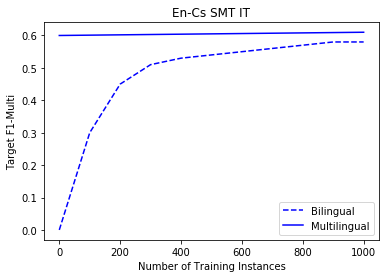
\includegraphics[width=\figlength]{figures/translation_quality_estimation/word_level/en_cs_smt_it.png}
		\caption{En-Cs SMT IT}
		\label{fig:en_cs_smt_results}
	\end{subfigure}
	\begin{subfigure}[b]{\figlength}
		\centering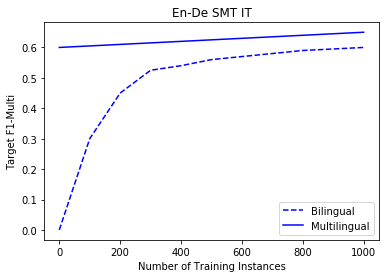
\includegraphics[width=\figlength]{figures/translation_quality_estimation/word_level/en_de_smt_it.png}
		\caption{En-De SMT IT}
		\label{fig:en_de_smt_it_results}
	\end{subfigure}
	\begin{subfigure}[b]{\figlength}
		\centering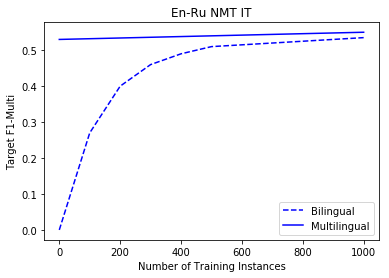
\includegraphics[width=\figlength]{figures/translation_quality_estimation/word_level/en_ru_nmt_it.png}
		\caption{En-Ru NMT IT}
		\label{fig:en_ru_nmt_it_results}
	\end{subfigure}
	\begin{subfigure}[b]{\figlength}
		\centering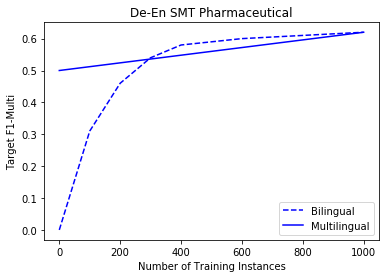
\includegraphics[width=\figlength]{figures/translation_quality_estimation/word_level/de_en_smt_pharm.png}
		\caption{De-En SMT Pharmaceutical}
		\label{fig:de_en_smt_pharm_results}
	\end{subfigure}
	\begin{subfigure}[b]{\figlength}
		\centering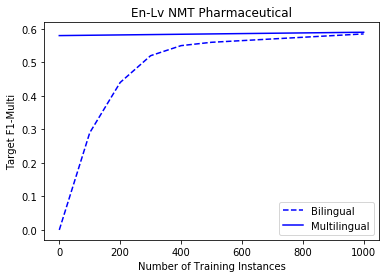
\includegraphics[width=\figlength]{figures/translation_quality_estimation/word_level/en_lv_nmt_pharm.png}
		\caption{En-Lv NMT Pharmaceutical}
		\label{fig:en_lv_nmt_Pharm_results}
	\end{subfigure}
	\begin{subfigure}[b]{\figlength}
		\centering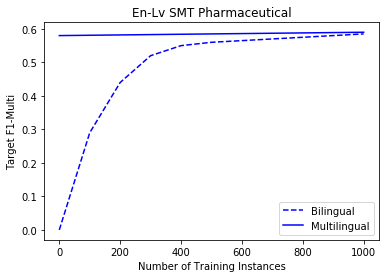
\includegraphics[width=\figlength]{figures/translation_quality_estimation/word_level/en_lv_smt_pharm.png}
		\caption{En-Lv SMT Pharmaceutical}
		\label{fig:en_lv_smt_pharm_results}
	\end{subfigure}
	\begin{subfigure}[b]{\figlength}
		\centering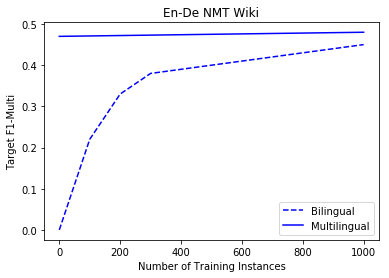
\includegraphics[width=\figlength]{figures/translation_quality_estimation/word_level/en_de_nmt_wiki.png}
		\caption{En-De NMT Wiki}
		\label{fig:en_de_nmt_wiki_results}
	\end{subfigure}
	\begin{subfigure}[b]{\figlength}
		\centering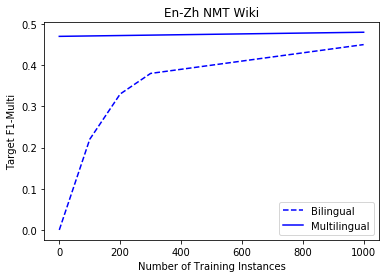
\includegraphics[width=\figlength]{figures/translation_quality_estimation/word_level/en_zh_nmt_wiki.png}
		\caption{En-Zh NMT Wiki}
		\label{fig:en_zh_nmt_wiki_results}
	\end{subfigure}
	\caption[Few-shot learning Results for Word-Level QE]{Few-shot learning Results for Word-Level QE. We report $F1_{\textit{MULTI}} \; Target$ scores against Number of training instances for multilingual and bilingual models.}
	\label{fig:fewshot_results}
\end{figure}

We also evaluated how the QE models behave with a limited number of training instances. For each language pair, we initiated the weights of the bilingual model with those of the relevant All-1 QE and trained it on 100, 200, 300 and up to 1000 training instances. We compared the results with those obtained, having trained the QE model from scratch for that language pair. The results in Figure \ref{fig:fewshot_results} show that All-1 or the multilingual model performs well above the QE model trained from scratch (Bilingual) when there is a limited number of training instances available. Even for the De-En language pair in sentence-level HTER QE and word-level QE, for which we had comparatively poor zero-shot results, the multilingual model provided better results with a few training instances. It seems that having the model weights already fine-tuned in the multilingual model provides an additional boost to the training process, which is advantageous in a few-shot scenario.

With these findings, we answer our \textbf{RQ3:} multilingual QE models perform better with a limited number of training instances (Few-shot learning) for an unseen language pair in both sentence-level and word-level QE. It is always better to transfer the weights from a multilingual QE model than to train the weights from scratch for a new language pair.


\section{Conclusion}
\label{sec:multilingual_conclusion}
The traditional way of having a single QE model for each language pair has many limitations; \textit{i. }They need to have annotated training data for each language pair which can be costly, \textit{ii. }Managing several QE models at the same time can be chaotic.  These limitations can hinder the ability of the state-of-the-art QE models to be applied in real-world applications. As a solution to that, we explored multilingual QE with state-of-the-art QE models. We used the sentence-level and word-level QE architectures in \textit{TransQuest} and evaluated them in different multilingual settings. 

In our experiments, we observed that multilingual QE models deliver excellent results on the language pairs they were trained on. In addition, the multilingual QE models perform well in the majority of the zero-shot scenarios where the multilingual QE model is tested on an unseen language pair. Furthermore, multilingual models perform very well with few-shot learning on an unseen language pair compared to training from scratch for that language pair, proving that multilingual QE models are effective even with a limited number of training instances. This suggests that we can train a single multilingual QE model on as many languages as possible and apply it to other language pairs. These findings can be beneficial to perform QE in low-resource languages for which the training data is scarce and when maintaining several QE models for different language pairs is arduous. Considering the benefits of multilingual models, we have released several multilingual sentence-level and word-level pre-trained models on HuggingFace model hub. 

The main limitation of our multilingual evaluation is that all the languages we used throughout the experiments are supported by the pre-trained XLM-R model we used. XLM-R large model only supports 100 languages at the moment, and there is a lot of low resource but common languages such as Chewa, Tajiki, Tigrinya\footnote{Chewa, Tajiki and Tigrinya are the official languages of Zimbabwe, Tajikistan and Eritrea respectively that are collectively spoken by more than 30 million people in the world} etc. that XLM-R does not support. A question can arise about how the language pairs that XLM-R does not support perform in our multilingual QE environment. However, as far as we know, until very recently, there were no annotated QE datasets either for the languages outside the 100 languages supported by XLM-R. Therefore, it would not be possible to carry out a proper evaluation. Very recently, in WMT 2021, an annotated QE dataset for Pashto-English and Khmer-English was introduced. XLM-R does not support Pashto and Khmer at the moment, and it would be interesting to experiment with them with our multilingual models, which we hope to do in future work.

Pre-trained multilingual transformer models are rapidly increasing in popularity in the NLP community. From them, one notable multilingual transformer model is mT5 \autocite{xue-etal-2021-mt5}; multilingual text to text transformer model, which considers every task as a sequence to sequence task. It has provided very good results in a variety of multilingual NLP tasks. As future work, we hope to incorporate mT5 in \textit{TransQuest} framework and evaluate it in a multilingual QE environment.

With this, we conclude Part III of the thesis, using deep learning based STS metrics in translation quality estimation. We showed that the state-of-the-art STS methods we experimented in Part I of the thesis can be employed successfully in QE. Our method outperform current neural QE models such as OpenKiwi and DeepQuest in word-level and sentence-level QE setting a new state-of-the-art. Furthermore, they are simple compared to the complex neural architectures employed in QE in recent years. We believe that the findings of Part III of the thesis would open a new direction in QE.






% Bibliography.
\addcontentsline{toc}{chapter}{Bibliography}
% Do not separate these files with spaces.

\renewcommand*{\bibfont}{\normalsize}
\renewcommand*{\nameyeardelim}{\addcomma\space}

\setlength\bibitemsep{10pt}
\printbibliography






% Appendix.
\appendix

\end{document}